\documentclass[a4paper,12pt,oneside,openleft]{memoir}

% Castellano
\usepackage[spanish,es-tabla,es-noshorthands]{babel}
\selectlanguage{spanish}
\usepackage[utf8]{inputenc}
\usepackage[T1]{fontenc}
\usepackage{lmodern} % scalable font
\usepackage{microtype}
\usepackage{placeins}

\RequirePackage{booktabs}
\RequirePackage[table]{xcolor}
\RequirePackage{xtab}
\RequirePackage{multirow}
\usepackage{tabularray}
\UseTblrLibrary{booktabs,varwidth}
\SetTblrInner[tblr,longtblr]{measure=hbox}
\usepackage{enumitem}

\usepackage{graphicx}
\usepackage{pdfpages}

% Formatear números
\usepackage{siunitx}
\sisetup{
  output-decimal-marker = {,},   % coma para decimales
  group-separator       = {.},   % punto para los miles
  group-minimum-digits  = 4      % agrupa desde 4 cifras: 1.000
}

% Manejar acrónimos
\usepackage{acronym}


% Links
\PassOptionsToPackage{hyphens}{url}\usepackage[colorlinks]{hyperref}
\hypersetup{
	allcolors = {black}
}
\usepackage{csquotes}
\usepackage[backend=biber,style=numeric,sorting=none]{biblatex}
\addbibresource{bibliografiaAnexos.bib}
\DeclareBibliographyAlias{standard}{manual}

% Ecuaciones
\usepackage{amsmath}

% Rutas de fichero / paquete
\newcommand{\ruta}[1]{{\sffamily #1}}

% Párrafos
\nonzeroparskip

% Huérfanas y viudas
\widowpenalty100000
\clubpenalty100000

% Evitar solapes en el header
\nouppercaseheads

% Imagenes
\newcommand{\imagen}[2]{
	\begin{figure}[!h]
		\centering
		\includegraphics[width=0.9\textwidth]{#1}
		\caption{#2}\label{fig:#1}
	\end{figure}
	\FloatBarrier
}

\newcommand{\imagenflotante}[2]{
	\begin{figure}%[!h]
		\centering
		\includegraphics[width=0.9\textwidth]{#1}
		\caption{#2}\label{fig:#1}
	\end{figure}
}

\graphicspath{{./img/}{./img/anexos/plan-de-proyecto-software/}}


% El comando \figura nos permite insertar figuras comodamente, y utilizando
% siempre el mismo formato. Los parametros son:
% 1 -> Porcentaje del ancho de página que ocupará la figura (de 0 a 1)
% 2 --> Fichero de la imagen
% 3 --> Texto a pie de imagen
% 4 --> Etiqueta (label) para referencias
% 5 --> Opciones que queramos pasarle al \includegraphics
% 6 --> Opciones de posicionamiento a pasarle a \begin{figure}
\newcommand{\figuraConPosicion}[6]{%
  \setlength{\anchoFloat}{#1\textwidth}%
  \addtolength{\anchoFloat}{-4\fboxsep}%
  \setlength{\anchoFigura}{\anchoFloat}%
  \begin{figure}[#6]
    \begin{center}%
      \Ovalbox{%
        \begin{minipage}{\anchoFloat}%
          \begin{center}%
            \includegraphics[width=\anchoFigura,#5]{#2}%
            \caption{#3}%
            \label{#4}%
          \end{center}%
        \end{minipage}
      }%
    \end{center}%
  \end{figure}%
}

%
% Comando para incluir imágenes en formato apaisado (sin marco).
\newcommand{\figuraApaisadaSinMarco}[5]{%
  \begin{figure}%
    \begin{center}%
    \includegraphics[angle=90,height=#1\textheight,#5]{#2}%
    \caption{#3}%
    \label{#4}%
    \end{center}%
  \end{figure}%
}
% Para las tablas
\newcommand{\otoprule}{\midrule [\heavyrulewidth]}
%
% Nuevo comando para tablas pequeñas (menos de una página).
\newcommand{\tablaSmall}[5]{%
 \begin{table}
  \begin{center}
   \rowcolors {2}{gray!35}{}
   \begin{tabular}{#2}
    \toprule
    #4
    \otoprule
    #5
    \bottomrule
   \end{tabular}
   \caption{#1}
   \label{tabla:#3}
  \end{center}
 \end{table}
}

%
%Para el float H de tablaSmallSinColores
\usepackage{float}

%
% Nuevo comando para tablas pequeñas (menos de una página).
\newcommand{\tablaSmallSinColores}[5]{%
 \begin{table}[H]
  \begin{center}
   \begin{tabular}{#2}
    \toprule
    #4
    \otoprule
    #5
    \bottomrule
   \end{tabular}
   \caption{#1}
   \label{tabla:#3}
  \end{center}
 \end{table}
}

\newcommand{\tablaApaisadaSmall}[5]{%
\begin{landscape}
  \begin{table}
   \begin{center}
    \rowcolors {2}{gray!35}{}
    \begin{tabular}{#2}
     \toprule
     #4
     \otoprule
     #5
     \bottomrule
    \end{tabular}
    \caption{#1}
    \label{tabla:#3}
   \end{center}
  \end{table}
\end{landscape}
}

%
% Nuevo comando para tablas grandes con cabecera y filas alternas coloreadas en gris.
\newcommand{\tabla}[6]{%
  \begin{center}
    \tablefirsthead{
      \toprule
      #5
      \otoprule
    }
    \tablehead{
      \multicolumn{#3}{l}{\small\sl continúa desde la página anterior}\\
      \toprule
      #5
      \otoprule
    }
    \tabletail{
      \hline
      \multicolumn{#3}{r}{\small\sl continúa en la página siguiente}\\
    }
    \tablelasttail{
      \hline
    }
    \bottomcaption{#1}
    \rowcolors {2}{gray!35}{}
    \begin{xtabular}{#2}
      #6
      \bottomrule
    \end{xtabular}
    \label{tabla:#4}
  \end{center}
}

%
% Nuevo comando para tablas grandes con cabecera.
\newcommand{\tablaSinColores}[6]{%
  \begin{center}
    \tablefirsthead{
      \toprule
      #5
      \otoprule
    }
    \tablehead{
      \multicolumn{#3}{l}{\small\sl continúa desde la página anterior}\\
      \toprule
      #5
      \otoprule
    }
    \tabletail{
      \hline
      \multicolumn{#3}{r}{\small\sl continúa en la página siguiente}\\
    }
    \tablelasttail{
      \hline
    }
    \bottomcaption{#1}
    \begin{xtabular}{#2}
      #6
      \bottomrule
    \end{xtabular}
    \label{tabla:#4}
  \end{center}
}

%
% Nuevo comando para tablas grandes sin cabecera.
\newcommand{\tablaSinCabecera}[5]{%
  \begin{center}
    \tablefirsthead{
      \toprule
    }
    \tablehead{
      \multicolumn{#3}{l}{\small\sl continúa desde la página anterior}\\
      \hline
    }
    \tabletail{
      \hline
      \multicolumn{#3}{r}{\small\sl continúa en la página siguiente}\\
    }
    \tablelasttail{
      \hline
    }
    \bottomcaption{#1}
  \begin{xtabular}{#2}
    #5
   \bottomrule
  \end{xtabular}
  \label{tabla:#4}
  \end{center}
}



\definecolor{cgoLight}{HTML}{EEEEEE}
\definecolor{cgoExtralight}{HTML}{FFFFFF}

%
% Nuevo comando para tablas grandes sin cabecera.
\newcommand{\tablaSinCabeceraConBandas}[5]{%
  \begin{center}
    \tablefirsthead{
      \toprule
    }
    \tablehead{
      \multicolumn{#3}{l}{\small\sl continúa desde la página anterior}\\
      \hline
    }
    \tabletail{
      \hline
      \multicolumn{#3}{r}{\small\sl continúa en la página siguiente}\\
    }
    \tablelasttail{
      \hline
    }
    \bottomcaption{#1}
    \rowcolors[]{1}{cgoExtralight}{cgoLight}

  \begin{xtabular}{#2}
    #5
   \bottomrule
  \end{xtabular}
  \label{tabla:#4}
  \end{center}
}


% Capítulos
\chapterstyle{bianchi}
\newcommand{\capitulo}[2]{
	\setcounter{chapter}{#1}
	\setcounter{section}{0}
	\setcounter{figure}{0}
	\setcounter{table}{0}
	\chapter*{#2}
	\addcontentsline{toc}{chapter}{#2}
	\markboth{#2}{#2}
}

% Apéndices
\renewcommand{\appendixname}{Apéndice}
\renewcommand*\cftappendixname{\appendixname}

\newcommand{\apendice}[1]{
	%\renewcommand{\thechapter}{A}
	\chapter{#1}
}

\renewcommand*\cftappendixname{\appendixname\ }

% Formato de portada
\makeatletter
\newcommand{\tutor}[1]{\def\@tutor{#1}}
\newcommand{\course}[1]{\def\@course{#1}}
\definecolor{cpardoBox}{HTML}{E6E6FF}
\def\maketitle{
  \null
  \thispagestyle{empty}
  % Cabecera ----------------
\noindent
\includegraphics[width=\textwidth]{institucional/cabecera}\vspace{1cm}%
  \vfill
  % Título proyecto y escudo informática ----------------
  \colorbox{cpardoBox}{%
    \begin{minipage}{.8\textwidth}
      \vspace{.5cm}\Large
      \begin{center}
      \textbf{TFG del \nombreGrado}\vspace{.6cm}\\
      \textbf{\LARGE\@title{}}
      \end{center}
      \vspace{.2cm}
    \end{minipage}

  }%
  \hfill\begin{minipage}{.20\textwidth}
    
\includegraphics[width=\textwidth]{institucional/escudo-informatica}
  \end{minipage}
  \vfill
  % Datos de alumno, curso y tutores ------------------
  \begin{center}%
  {%
    \noindent\LARGE
    Presentado por \@author{}\\
    en \nombreUniversidad\\
    \@date{}\\
    Tutor: \@tutor{}\\[.6em]
    Cotutores empresariales:\\[.2em]
    \tutoresEmpresariales\\
  }%
  \end{center}%
  \null
  \cleardoublepage
  }
\makeatother

% Se definen los datos generales del documento.
\newcommand{\titulo}{Manualito}
\newcommand{\subtitulo}{Aplicación web de apoyo al aprendizaje de juegos de mesa}
\newcommand{\nombre}{Ibai Moya Aroz}
\newcommand{\dni}{DNI CENSORED}
\newcommand{\nombreTutor}{Bruno Baruque Zanón}
\newcommand{\tutoresEmpresariales}{Pablo García Ullán,\\Luis Peralta\\y Ánder Bermúdez González}
\newcommand{\departamentoTutor}{Departamento de Ingeniería Informática}
\newcommand{\areaTutor}{Área de Lenguajes y Sistemas Informáticos}
\newcommand{\fechaEntrega}{17 de septiembre de 2026}
\newcommand{\nombreGrado}{Grado en Ingeniería Informática}
\newcommand{\ciudad}{Burgos}
\newcommand{\nombreUniversidad}{Universidad de \ciudad}


% Datos de portada.
\title{{\Huge \titulo}\\[0.5cm]\subtitulo\\[0.4cm]{\Large Documentación técnica}}
\author{\nombre}
\tutor{\nombreTutor}
\date{\fechaEntrega}


\begin{document}

\maketitle



\cleardoublepage



%%%%%%%%%%%%%%%%%%%%%%%%%%%%%%%%%%%%%%%%%%%%%%%%%%%%%%%%%%%%%%%%%%%%%%%%%%%%%%%%%%%%%%%%



\frontmatter


\clearpage

% Indices
\tableofcontents

\clearpage

\listoffigures

\clearpage

\listoftables

\clearpage

\chapter*{Lista de acrónimos}
\addcontentsline{toc}{chapter}{Lista de acrónimos}
\begin{acronym}[WWWWW] % plantilla de la sigla más ancha, para alinear
    \acro{AGPL}{GNU Affero General Public License}
    \acro{API}{\textit{Application Programming Interface}}
    \acro{BM25}{\textit{Best Match 25}}
    \acro{BSD}{Berkeley Software Distribution}
    \acro{BSL}{Business Source License}
    \acro{CD}{\textit{Continuous Deployment}}
    \acro{CI}{\textit{Continuous Integration}}
    \acro{CPU}{\textit{Central Processing Unit}}
    \acro{CRUE}{Conferencia de Rectores de las Universidades Españolas}
    \acro{CSRF}{\textit{Cross-Site Request Forgery}}
    \acro{CUDA}{\textit{Compute Unified Device Architecture}}
    \acro{cuDNN}{\textit{CUDA Deep Neural Network}}
    \acro{E2E}{\textit{End-to-End}}
    \acro{FK}{\textit{Foreign Key}}
    \acro{GPU}{\textit{Graphics Processing Unit}}
    \acro{HNSW}{\textit{Hierarchical Navigable Small World}}
    \acro{HTML}{\textit{HyperText Markup Language}}
    \acro{IA}{Inteligencia artificial}
    \acro{IEC}{International Electrotechnical Commission}
    \acro{IEEE}{Institute of Electrical and Electronics Engineers}
    \acro{ISC}{Internet Software Consortium}
    \acro{ISO}{International Organization for Standardization}
    \acro{LGPL}{GNU Lesser General Public License}
    \acro{LLM}{\textit{Large Language Model}}
    \acro{MIT}{Massachusetts Institute of Technology}
    \acro{ML}{\textit{Machine Learning}}
    \acro{MVP}{\textit{Minimum Viable Product}}
    \acro{OCR}{\textit{Optical Character Recognition}}
    \acro{OFL}{Open Font License}
    \acro{OSS}{\textit{Open Source Software}}
    \acro{PDF}{\textit{Portable Document Format}}
    \acro{PK}{\textit{Primary Key}}
    \acro{PWA}{\textit{Progressive Web App}}
    \acro{QA}{\textit{Quality Assurance}}
    \acro{RAG}{\textit{Retrieval-Augmented Generation}}
    \acro{ReDoS}{\textit{Regular Expression Denial of Service}}
    \acro{RRF}{\textit{Reciprocal Rank Fusion}}
    \acro{RSAL}{Redis Source Available License}
    \acro{SaaS}{\textit{Software as a Service}}
    \acro{SSPL}{Server Side Public License}
    \acro{TDD}{\textit{Test-Driven Development}}
    \acro{TTS}{\textit{Text-To-Speech}}
    \acro{UML}{\textit{Unified Modeling Language}}
    \acro{WCAG}{\textit{Web Content Accessibility Guidelines}}
    \acro{XSS}{\textit{Cross-Site Scripting}}
\end{acronym}
\clearpage

\mainmatter

\appendix

\apendice{Plan de Proyecto \textit{Software}}


\section{Introducción}

La fase de planificación es una de las más críticas de cualquier proyecto
\textit{software}. En ella se estima el trabajo, el tiempo y el coste que puede
suponer su realización, para lo cual es necesario analizar con detalle cada
una de las partes que lo componen. Además de permitir estimar los recursos
necesarios, este análisis facilita y agiliza la toma de decisiones en las
etapas futuras del desarrollo.

Normalmente, la planificación de un proyecto se separa en dos partes:

\begin{itemize}
    \item A la parte que organiza el trabajo a lo largo del tiempo se le
    denomina \textbf{planificación temporal}.
    \item A la parte que evalúa si el proyecto es realista y factible
    se le denomina \textbf{estudio de viabilidad}.
\end{itemize}

En la planificación temporal se elabora un programa de tiempos en el que se
estima la duración de cada tarea del proyecto. Además, se fijan una \textbf{fecha
de inicio}, una \textbf{fecha de finalización estimada}, que se suele fijar
algo antes de la fecha límite para congelar el desarrollo de nuevas
funcionalidades y poner como objetivo probar el producto y detectar errores y,
por último, la \textbf{fecha límite}, que coincide con la fecha pactada con el
cliente para entregar el producto finalizado de acuerdo con los requisitos
indicados por este.

A la hora de estimar tiempos es importante no solo basarse en experiencias
previas con tareas similares, sino también tener en cuenta que ciertas
tareas pueden estar en una situación de bloqueo hasta que otras terminen.

Por otra parte, el estudio de viabilidad determina si completar el proyecto,
tanto a nivel legal, como dentro de los plazos establecidos con ciertos límites económicos es algo
realista, por lo tanto, se divide en dos apartados:

\begin{itemize}
    \item La parte que estima los costes que conlleva desarrollar el
    proyecto y sus posibles beneficios se conoce como \textbf{viabilidad
    económica}.
    \item La parte que analiza los apartados legales que pudiesen reportar
    conflictos, como por ejemplo las licencias de las diferentes herramientas
    que se van a usar, se conoce como \textbf{viabilidad legal}.


\end{itemize}

\section{Planificación temporal}
La entrega está prevista para el \fechaEntrega. El registro de trabajo
comienza el 26 de febrero de 2026, por lo que la estimación económica toma
como referencia los \num{204} días naturales comprendidos entre ambas
fechas, incluidas las dos. Las fechas y horas de los \textit{Sprints}
recogen el seguimiento realizado, mientras que la fecha de entrega fija el
límite previsto para completar el desarrollo y la documentación.

Para la planificación temporal se ha seguido una \textbf{metodología ágil}
adaptada a las características y necesidades del proyecto. El desarrollo
se ha dividido en iteraciones, denominadas \textit{Sprints}. Cada una de
ellas se estructuraba en torno a una reunión de equipo en la que se exponían
\textbf{los puntos tratados} durante dicha iteración, \textbf{los problemas}
que habían surgido a raíz del desarrollo de las tareas y, por último,
\textbf{los objetivos previstos} de cara al cierre de la siguiente iteración.

La duración de cada \textit{Sprint} ha sido de \textbf{2 semanas}, salvo en
algunas iteraciones concretas, en las que surgieron imprevistos.

Para organizar las tareas propuestas en cada \textit{Sprint} se ha usado un
\textbf{\textit{tablero Kanban}} en el que se iba marcando cuando se estaba
trabajando en una tarea o cuando se podía dar por finalizada.

En los siguientes apartados se detalla cada uno de los \textit{Sprints} por
separado.

\subsection{\textit{Sprint} 0: Planteamiento inicial e investigación}
\textbf{Duración:} del 26 de febrero al 12 de marzo de 2026.
Este \textit{Sprint} dio comienzo oficialmente al proyecto, aunque es cierto
que se realizó un estudio de viabilidad mínimo previo a este proyecto. En la
reunión inicial se explicó la idea más a fondo y se debatió qué dirección se
quería que tomase el proyecto desde el principio. Por tanto, este \textit{Sprint}
se centró en investigar y recopilar información útil para asentar una buena base
y en empezar a montar el principio del \textit{pipeline}, comenzando por el
\textbf{reconocimiento óptico de caracteres} (\acs{OCR}, del inglés \textit{Optical Character
Recognition})\acused{OCR}.

El desglose en tareas junto con los campos asociados a cada una se
recoge en la figura~\ref{fig:sprint-00}.

\imagen{sprint-00}{Tablero del \textit{Sprint} 0.}

Se emplearon 13 horas y media de las 17 estimadas, y se completaron todas las
tareas previstas.

\subsection{\textit{Sprint} 1: Arquitectura base, CI y módulo OCR}
\textbf{Duración:} del 12 de marzo al 26 de marzo de 2026.
Con una idea más asentada acerca de la dirección del proyecto, este \textit{Sprint}
se centró en configurar el repositorio y su \textbf{integración continua} (CI, del
inglés \textit{Continuous Integration})\acused{CI}. Además, se creó una base de
arquitectura sobre la que empezar a desarrollar las funcionalidades.
Por otro lado, se investigaron y probaron diferentes opciones de \ac{OCR}, de
\textbf{generación aumentada por recuperación}
(\acs{RAG}, del inglés \textit{Retrieval-Augmented Generation})\acused{RAG}
y de \textbf{grandes modelos de lenguaje}
(\acs{LLM}, del inglés \textit{Large Language Model})\acused{LLM}.

El desglose en tareas junto con los campos asociados a cada una se
recoge en la figura~\ref{fig:sprint-01}.

\imagen{sprint-01}{Tablero del \textit{Sprint} 1.}

Se emplearon 24 horas de las 24 estimadas, y se completaron todas las
tareas previstas.

\subsection{\textit{Sprint} 2: Migración a microservicios, RAG y LLM}
\textbf{Duración:} del 26 de marzo al 16 de abril de 2026.
Este \textit{Sprint} se centró en pulir la estructura base del proyecto
y migrar la arquitectura monolítica a una arquitectura de
microservicios, en la que se planteó mover cada elemento lo
suficientemente grande, como por ejemplo, el \ac{LLM} o el \ac{OCR},
a su propio módulo en el que poder modificarse o instalar dependencias
sin afectar al resto del sistema~\cite{fowler_microservices}.
Adicionalmente, se hizo uso de esta nueva arquitectura para montar la
primera versión del \textit{pipeline}, conectando el \ac{RAG} con el \ac{LLM}.

El desglose en tareas junto con los campos asociados a cada una se
recoge en la figura~\ref{fig:sprint-02}.

\imagen{sprint-02}{Tablero del \textit{Sprint} 2.}

Se emplearon 28 horas frente a las 20 estimadas, y se completaron todas las
tareas previstas.

\subsection{\textit{Sprint} 3: Estabilización y optimización del motor de IA}
\textbf{Duración:} del 16 de abril al 23 de abril de 2026.

Este \textit{Sprint} se centró en mejorar la estabilidad y optimizar el motor de
\ac{IA} de la aplicación, formado por el \ac{RAG} y el \ac{LLM}. Para ello, se
establecieron una serie de requisitos y se siguió un enfoque de desarrollo guiado
por pruebas (\acs{TDD}, del inglés \textit{Test-Driven Development})\acused{TDD}~\cite{agile_alliance_tdd},
con el objetivo de validar el comportamiento esperado de dichos módulos.

Por otro lado, se hizo un análisis del estado del arte de \textbf{modelos de
síntesis de voz} (\acs{TTS}, del inglés \textit{Text-To-Speech})\acused{TTS} y un
estudio de viabilidad mínimo, sobre todo de cara a las limitaciones a nivel de
\textit{hardware} disponible.

El desglose en tareas junto con los campos asociados a cada una se
recoge en la figura~\ref{fig:sprint-03}.

\imagen{sprint-03}{Tablero del \textit{Sprint} 3.}

Se emplearon 15 horas frente a las 12 estimadas, y se completaron todas las
tareas previstas.

\subsection{\textit{Sprint} 4: Creación de un \textit{frontend} básico funcional}
\textbf{Duración:} del 23 de abril al 12 de mayo de 2026.

Este \textit{Sprint} se centró en refactorizar el \textit{backend}, aplicando
patrones de diseño y buenas prácticas. Por ejemplo, se emplearon patrones como \textbf{\textit{Strategy}} y \textbf{\textit{Factory}}~\cite{patterns}. El
primero sirve para encapsular los distintos motores de \ac{OCR} tras una interfaz
común e intercambiarlos sin afectar al resto del sistema, y el segundo para
instanciar el motor adecuado según la configuración.

Por otro lado, se implementaron en el flujo de \ac{CI} herramientas como
\textbf{\textit{Ruff}}~\cite{ruff} para mejorar la calidad del código.

Sobre esa base, se conectó una interfaz sencilla en \acs{HTML} (del inglés
\textit{HyperText Markup Language})\acused{HTML} con la que disponer de una demo y probar el \textit{pipeline} de \textbf{extremo a
extremo} (\acs{E2E}, del inglés \textit{End-to-End})\acused{E2E}.

La primera interfaz web de demostración se muestra en la figura~\ref{fig:sprint-04-demo-frontend}.

\imagen{sprint-04-demo-frontend}{Interfaz web de demostración desarrollada para probar el \textit{pipeline} de extremo a extremo.}

En la reunión se debatió acerca del estudio de viabilidad del módulo de \ac{TTS}
y, finalmente, se decidió dejarlo fuera debido a las limitaciones de
\textit{hardware} y a la complejidad y la pérdida de calidad en
la experiencia de usuario que supondría un sistema de carga y descarga de modelos
para gestionar los recursos.

El desglose en tareas junto con los campos asociados a cada una se
recoge en la figura~\ref{fig:sprint-04}.

\imagen{sprint-04}{Tablero del \textit{Sprint} 4.}

Se emplearon 20 horas y 40 minutos frente a las 20 estimadas, y se
completaron todas las tareas previstas.

\subsection{\textit{Sprint} 5: Refinamiento del \textit{backend} y diseño del \textit{frontend}}
\textbf{Duración:} del 12 de mayo al 26 de mayo de 2026.

Este \textit{Sprint} se centró principalmente en desarrollar la primera versión de
una \textbf{aplicación web progresiva} (\acs{PWA}, del inglés
\textit{Progressive Web App})\acused{PWA} y sentar las bases para mejorarla en
futuras iteraciones~\cite{mdn_pwa}.

Adicionalmente, como resultado de haber realizado la demo, se observó que, pese a
que el motor \textit{\textbf{PaddleOCR}}~\cite{paddleocr_tech_report} que se estaba
utilizando era muy fiable en cuanto a los resultados, era considerablemente lento. Además,
su variante adaptada para la \textbf{\textit{Unidad de Procesamiento Gráfico}}
(\acs{GPU}, del inglés \textit{Graphics Processing Unit})\acused{GPU}, con la que se reducía el
problema de rendimiento, es muy dependiente de las versiones de \acs{CUDA} (del inglés
\textit{Compute Unified Device Architecture})\acused{CUDA}, \textit{PaddlePaddle} y de los
\textit{drivers} de la \ac{GPU}~\cite{paddlepaddle_install}. Por motivos de compatibilidad,
se decidió añadir el motor \ac{OCR} \textbf{\textit{Tesseract}}~\cite{tesseract_ocr} como
opción por defecto y haciendo uso de los patrones de diseño aplicados que permiten tener
varias opciones configurables~\cite{patterns}, tras haber sido el mejor motor en promedio
en las medidas tomadas en los \textit{benchmarks} realizados.


Por último, se implementó \textit{SonarQube}~\cite{sonarqube_ci} como un paso más de
\ac{CI} con el objetivo de
reducir \textit{code smells}~\cite{sonarqube_metrics} y malas prácticas en el código.
Utilizando esta nueva herramienta, en este mismo \textit{Sprint} se aprovechó para
corregir la \textbf{deuda técnica}~\cite{sonarqube_metrics} detectada por
\textit{SonarQube}.

El desglose en tareas junto con los campos asociados a cada una se
recoge en la figura~\ref{fig:sprint-05}.
\imagen{sprint-05}{Tablero del \textit{Sprint} 5.}

Se emplearon 81 horas y 7 minutos frente a las 58 estimadas, y se
completaron todas las tareas previstas.

\subsection{\textit{Sprint} 6: Finalización del MVP}
\textbf{Duración:} del 26 de mayo al 13 de junio de 2026.

Este \textit{Sprint} se centró en montar \textbf{\textit{una base de datos relacional en
PostgreSQL}}~\cite{postgresql_about}, sobre la que almacenar manuales, \textit{assets},
conversaciones, etc.

La parte más importante de este paso se encontraba en crear un \textbf{sistema de usuarios},
haciendo especial énfasis en su \textbf{seguridad} teniendo en cuenta apartados
como \textbf{la gestión de sesiones}~\cite{owasp_session_management}, o la \textbf{protección
contra falsificación de peticiones entre sitios web} (\acs{CSRF}, del inglés \textit{Cross-Site
Request Forgery})\acused{CSRF}~\cite{owasp_csrf} entre otros.
Estas medidas se detallan en el apartado
\guillemotleft{}\nameref{sec:diseno-seguridad}\guillemotright{} del anexo de diseño.

Al mismo tiempo, se puso como objetivo mejorar el \textit{frontend} y la experiencia de
usuario mediante iteraciones hasta llegar a tener un \textbf{producto mínimo viable}
(\acs{MVP}, del inglés \textit{Minimum Viable Product})\acused{MVP}~\cite{agile_alliance_mvp}, incluyendo
apartados como el rendimiento, la flexibilidad y la robustez, tal como se puede ver en el
desglose de tareas al ampliar la cantidad de \textit{assets} y formatos soportados o al reducir
el tamaño y tiempo de construcción de las imágenes \textit{Docker}.

El desglose en tareas junto con los campos asociados a cada una se
recoge en la figura~\ref{fig:sprint-06}.

\imagen{sprint-06}{Tablero del \textit{Sprint} 6.}

Se emplearon 151 horas y 40 minutos frente a las 77 estimadas, y se
completaron todas las tareas previstas.

\subsection{\textit{Sprint} 7: Preparación del despliegue}
\textbf{Duración:} del 15 de junio al 30 de junio de 2026.

Este \textit{Sprint} se centró sobre todo en dejar todo preparado para el despliegue
de la aplicación. Para ello, se llevó a cabo una fase de
\textbf{aseguramiento de la calidad} (\acs{QA}, del inglés
\textit{Quality Assurance})\acused{QA}~\cite{iso_quality_assurance}.

Durante dicha fase, se detectaron principalmente tres problemas:

\begin{itemize}
    \item El procesamiento de tareas pesadas estaba bloqueando el
    \textbf{bucle de eventos principal de la aplicación}.
    \item La calidad de los resultados del \ac{OCR} era, en ocasiones,
    \textbf{insuficiente} para enriquecer las respuestas del \ac{LLM}
    \item La aplicación requería de un \textit{hardware} muy específico.
\end{itemize}

Una vez identificados, se crearon tareas para investigar posibles soluciones,
implementarlas y comprobar que corregían los problemas detectados.

La ejecución tareas pesadas se movieron a una \textbf{cola de Celery}, utilizando Redis como \textit{broker} de mensajes~\cite{celery_introduction}.

Para mejorar los resultados del \ac{OCR}, se creó un \textit{pipeline} que
aplica un \textbf{preprocesado de imagen} específico para cada motor.

Por último, se añadió un arranque adaptativo que detecta la disponibilidad de
una GPU NVIDIA y la VRAM libre para recomendar perfiles compatibles del \ac{LLM}
y del \ac{OCR}.

El desglose en tareas junto con los campos asociados a cada una se
recoge en la figura~\ref{fig:sprint-07}.

\imagen{sprint-07}{Tablero del \textit{Sprint} 7.}

Se emplearon 82 horas frente a las 82 estimadas, y se completaron todas
las tareas previstas.

\subsection{\textit{Sprint} 8: Despliegue de la aplicación}
\textbf{Duración:} del 1 de julio al 20 de julio de 2026.

Este \textit{Sprint} se centró en crear la infraestructura necesaria para
realizar el primer despliegue de \textit{Manualito}, tanto del sitio web de
presentación (desplegado en \href{https://manualito.dev/}{\textit{manualito.dev}})
como de la aplicación a través de \textit{Cloudflare
Tunnel}~\cite{cloudflare_tunnel}
(desplegado a demanda en \href{https://app.manualito.dev/}{\textit{app.manualito.dev}}).

Como consecuencia de preparar el proyecto para su publicación, se estableció un
flujo de trabajo basado en \textbf{ramas por entorno}~\cite{gitlab_branch_per_environment}
para organizar el desarrollo, las pruebas y el despliegue de los cambios.

Además, los \textit{runners} de GitLab alojados en la infraestructura de HP SCDS
comenzaron a fallar, lo que impedía mantener el flujo de \ac{CI} e implementar un
procedimiento fiable de \textbf{despliegue continuo} (\acs{CD}, del inglés
\textit{Continuous Deployment})\acused{CD}. Por este motivo, el repositorio
principal se migró a GitHub~\cite{manualito_github}. Por su parte, GitLab se
mantuvo para conservar la trazabilidad del proyecto, por lo que las
\textit{issues} se replicaron en ambas plataformas~\cite{manualito_gitlab}.

El desglose en tareas junto con los campos asociados a cada una se
recoge en la figura~\ref{fig:sprint-08}.

\imagen{sprint-08}{Tablero del \textit{Sprint} 8.}

Se emplearon 68 horas y 35 minutos frente a las 75 estimadas, y se
completaron todas las tareas previstas.

\subsection{\textit{Sprint} 9: Despliegue de la documentación}
\textbf{Duración:} del 20 de julio al 6 de agosto de 2026.

Este \textit{Sprint} se centró en crear un sitio web en el que publicar la
documentación de \textit{Manualito}. Para ello, se utilizó \textit{Starlight},
un tema de documentación basado en \textit{Astro}~\cite{starlight_documentation}, para exponer las guías de uso y la documentación técnica del proyecto.

El sitio se desplegó mediante
\textit{Cloudflare Workers Static Assets}~\cite{cloudflare_workers_static_assets}
y se publicó en \href{https://docs.manualito.dev/}{\textit{docs.manualito.dev}}.

Por otro lado, se internacionalizó la interfaz de \textit{Manualito} para que
pudiera utilizarse \textbf{tanto en español como en inglés}.

El desglose en tareas junto con los campos asociados a cada una se
recoge en la figura~\ref{fig:sprint-09}.

\imagen{sprint-09}{Tablero del \textit{Sprint} 9.}

Se emplearon 50 horas y 30 minutos frente a las 53 estimadas, y se
completaron todas las tareas previstas.

\subsection{\textit{Sprint} 10: Mejora del \acs{RAG}}
\textbf{Duración:} del 6 de agosto al 23 de agosto de 2026.

Este \textit{Sprint} se centró en mejorar el \ac{RAG} de \textit{Manualito}.
Para ello, se combinaron las \textbf{búsquedas semánticas y textuales}, y se
incorporó el nombre del juego a la consulta para interpretar preguntas que
no lo mencionaban explícitamente.

Además, se aplicó el filtro de \textbf{manuales autorizados} antes de
recuperar los fragmentos, para que los documentos que el usuario no podía
consultar no ocupasen posiciones entre los resultados.

Por último, se añadió una tarea periódica para mantener el índice de
búsqueda sincronizado con PostgreSQL, eliminando las entradas de manuales
borrados y repitiendo las indexaciones incompletas.

El desglose en tareas junto con los campos asociados a cada una se
recoge en la figura~\ref{fig:sprint-10}.

\imagen{sprint-10}{Tablero del \textit{Sprint} 10.}

Se emplearon 47 horas frente a las 115 estimadas, y se completaron todas las tareas previstas.

\subsection{\textit{Sprint} 11: Redacción de la documentación}
\textbf{Duración:} del 23 de agosto al 17 de septiembre de 2026.

Este \textit{Sprint} se centró en recopilar y completar la documentación
redactada durante el desarrollo para preparar la \textbf{memoria y los anexos
del trabajo de fin de grado}. También se publicaron los estudios de rendimiento
del proyecto y se corrigieron pequeños errores e incoherencias detectados al
revisar la interfaz y el envío de correos.

El desglose en tareas junto con los campos asociados a cada una se
recoge en la figura~\ref{fig:sprint-11}.

\imagen{sprint-11}{Tablero del \textit{Sprint} 11.}

El tiempo dedicado a la memoria y los anexos se repartió entre numerosas sesiones
breves, por lo que no se conserva una medición suficientemente precisa de las
horas empleadas. Para evitar establecer una cifra reconstruida sin evidencia,
no se incluye una estimación del esfuerzo de este \textit{Sprint}.

\section{Estudio de viabilidad}

Una vez planificado el trabajo en el tiempo, queda comprobar que el proyecto
se puede realizar. Para ello se analizan los dos apartados que mencionados
anteriormente: la \textbf{viabilidad económica}, que estima los costes de
desarrollo y los contrasta con los beneficios esperables, y la \textbf{viabilidad
legal}, que revisa las licencias de las herramientas empleadas y el cumplimiento
normativo aplicable.

\subsection{Viabilidad económica}
El presupuesto estima cuánto costaría desarrollar \textit{Manualito} en un
entorno empresarial, aunque el proyecto se haya realizado en un contexto
académico. Para valorar el trabajo se mantiene la hipótesis de un
desarrollador a jornada completa durante el periodo previsto, del 26 de
febrero al \fechaEntrega.

El personal, las amortizaciones y la conexión a internet se prorratean mediante el factor
\(\num{204}/\num{365}\), correspondiente a los días del periodo y del año
2026. Las cuotas mensuales se convierten primero a su equivalente anual.
Así se incluyen los meses parciales sin redondear la duración a meses
completos. Los importes se redondean a céntimos antes de sumar las filas de
cada tabla.

\subsubsection{Costes}
La estimación reúne el coste de personal, la parte del equipo y las licencias
imputada al proyecto, y los gastos de electricidad, conexión y entrega.

\noindent\textbf{Costes de personal}\par
Se considera un único desarrollador de perfil \textit{junior} a jornada
completa. Como referencia mínima se toma el \textbf{Salario Mínimo
Interprofesional} de 2026, fijado en \num{17094.00}\,€ anuales~\cite{smi2026}.
Esta cantidad sirve como base del presupuesto, sin equipararla al salario de
mercado de ese perfil.

Sobre esa base se estima una cotización empresarial del
\qty{30.65}{\percent}, suponiendo una contratación indefinida. El porcentaje
reúne las contingencias comunes (\qty{23.60}{\percent}), el desempleo
(\qty{5.50}{\percent}), el Mecanismo de Equidad Intergeneracional
(\qty{0.75}{\percent}), el Fondo de Garantía Salarial
(\qty{0.20}{\percent}) y la formación profesional
(\qty{0.60}{\percent})~\cite{orden_cotizacion_2026}.

Se trata de una aproximación presupuestaria. Una contratación real exigiría
comprobar la base mínima del grupo profesional y añadir la cotización por
accidentes de trabajo y enfermedades profesionales, cuya tarifa depende de
la actividad. Tampoco se contemplan horas extraordinarias ni complementos
salariales.

La tabla~\ref{tabla:costes-personal} recoge la referencia anual y el importe
imputado a los \num{204} días del proyecto.
\tablaSmallSinColores
  {Costes de personal.}
  {l S[table-format=5.2, detect-weight]}
  {costes-personal}
  {\textbf{Concepto} & {\textbf{Coste (€)}} \\}
  {
    Salario bruto anual                       & \num{17094.00} \\
    Cotización empresarial anual              & \num{5239.31} \\
    Coste empresarial anual estimado           & \num{22333.31} \\
    \midrule
    Salario bruto del periodo                 & \num{9553.91} \\
    Cotización empresarial del periodo        & \num{2928.27} \\
    \midrule
    \bfseries Total (204 días)                & \bfseries \num{12482.18} \\
  }

\noindent\textbf{Costes de componentes \textit{hardware}}\par

 El siguiente paso es revisar todos los gastos derivados de componentes \textit{hardware}
 que se necesitan para desarrollar y probar un producto \textit{software} de este tipo. En
 este caso es especialmente relevante, ya que a la hora de tratar con modelos \ac{IA}
 como los \ac{LLM} se necesitan ciertas capacidades de computación que idealmente se
 obtienen de una \ac{GPU} que cuente con la suficiente potencia.

A continuación se desglosan los componentes y costes asociados que podría tener un equipo
con la potencia necesaria~\ref{tabla:costes-hardware}.

\tablaSmallSinColores
  {Costes de componentes \textit{hardware}.}
  {l r r}
  {costes-hardware}
  {\textbf{Componente} & \textbf{Precio (€)} & \textbf{Amortizado (€)} \\}
  {
    Procesador AMD Ryzen 5 7600             & \num{174.90}  & \num{24.44}  \\
    \ac{GPU} NVIDIA RTX 4070 Super          & \num{639.90}  & \num{89.41}  \\
    Memoria RAM 32\,GB DDR5                 & \num{184.98}  & \num{25.85}  \\
    Placa base AM5 (B850)                   & \num{129.90}  & \num{18.15}  \\
    SSD NVMe PCIe 4.0 1\,TB                 & \num{154.95}  & \num{21.65}  \\
    Fuente 750\,W 80+ Gold                  & \num{112.99}  & \num{15.79}  \\
    Disipador por aire AM5                  & \num{21.95}   & \num{3.07}   \\
    Caja ATX                                & \num{79.90}   & \num{11.16}   \\
    \midrule
    \bfseries Total                         & \bfseries\num{1499.47} & \bfseries\num{209.52} \\
  }

Los precios se han consultado en PcComponentes a fecha de 20 de junio de 2026 ~\cite{pccomp_ryzen_7600,
pccomp_rtx_4070_super,pccomp_ram_kingston_32gb,pccomp_msi_b850,
pccomp_kingston_nv3,pccomp_msi_a750gl,pccomp_hyper_212,pccomp_corsair_3000d}.

Para estimar la parte del equipo consumida durante el proyecto se adopta
una amortización lineal con una vida útil de cuatro años (\num{48} meses),
valor residual nulo e imputación íntegra durante el periodo considerado.
Esta vida útil equivale al coeficiente anual del \qty{25}{\percent}
recogido para los equipos informáticos en la tabla del impuesto sobre
sociedades~\cite{ley_impuesto_sociedades}, que se utiliza como referencia.
El coste de cada componente se calcula como:
\[
  \text{Coste amortizado} = \text{Precio} \times
  \frac{\num{204}}{\num{365} \times \num{4}}
\]

\noindent\textbf{Costes de licencias \textit{software}}\par

Otro punto importante es revisar los gastos en licencias de programas, si bien la
gran mayoría de \textit{software} utilizado es de código abierto (\acs{OSS}, del
inglés \textit{Open Source Software})\acused{OSS}, el desarrollo y las pruebas
se han realizado sobre \textit{Windows}, lo que requiere una licencia de
\textit{Windows 11 Pro}~\cite{ms_windows11_pro}.

Los precios de las licencias de \textit{software} se desglosan en la siguiente
tabla~\ref{tabla:costes-software}.

\tablaSmallSinColores
  {Costes de las licencias \textit{software}.}
  {l S[table-format=3.2] S[table-format=2.2]}
  {costes-software}
  {\textbf{\textit{Software}} & {\textbf{Precio (€)}} & {\textbf{Amortizado (€)}} \\}
  {
    Windows 11 Pro                         & \num{259.00} & \num{48.25} \\
    \midrule
    \bfseries Total                        & \bfseries \num{259.00} & \bfseries \num{48.25} \\
  }

Para la licencia se adopta una vida útil de tres años (\num{36} meses),
con amortización lineal y valor residual nulo. Es una hipótesis del
presupuesto, por lo que el importe imputado se obtiene mediante
\(\num{259.00} \times \num{204}/(\num{365} \times \num{3})\), que resulta
en \num{48.25}\,€.

\noindent\textbf{Otros costes}\par
El consumo eléctrico se aproxima a partir del esfuerzo registrado. Los
\textit{Sprints} 0 a 9 suman \num{535} horas y \num{2} minutos entre el
26 de febrero y el 6 de agosto, un periodo de \num{162} días naturales.
Para estimar el consumo hasta la entrega se mantiene ese ritmo medio
durante los \num{204} días previstos:
\[
  \text{Horas estimadas} =
  \left(\num{535} + \frac{\num{2}}{\num{60}}\right)
  \times \frac{\num{204}}{\num{162}}
  \simeq \num{673.75}
\]

Suponiendo que el equipo se utiliza durante esas horas, con una potencia
media de \qty{250}{\watt} y un precio de \num{0.15}\,€/kWh~\cite{ocu_precio_luz},
el coste estimado es de \num{25.27}\,€. De ese importe, \num{20.06}\,€
corresponden al esfuerzo ya registrado y \num{5.21}\,€ a la prolongación del
mismo ritmo hasta la entrega. Esta aproximación no equivale a una medición
del consumo ni añade horas al registro de los \textit{Sprints}.

Para la conexión a internet se conserva una cuota de
\num{30}\,€ mensuales~\cite{jazztel_fibra} y se imputa al proyecto un
\qty{30}{\percent} del uso, al compartirla con actividades personales.
Aplicando el mismo periodo que al resto del presupuesto, el cálculo es
\(\num{30} \times \num{12} \times \num{204}/\num{365}
\times \num{0.30} = \num{60.36}\)\,€.

La impresión y encuadernación se estiman en \num{50}\,€ como gasto puntual.
Para el registro del dominio \textit{manualito.dev} se reserva una anualidad
de \num{12}\,€.


Todo esto se desglosa en la tabla~\ref{tabla:otros-costes}.

\tablaSmallSinColores
  {Otros costes.}
  {l S[table-format=3.2]}
  {otros-costes}
  {\textbf{Concepto} & {\textbf{Coste (€)}} \\}
  {
    Consumo eléctrico                        & \num{25.27} \\
    Conexión a internet                      & \num{60.36} \\
    Impresión y encuadernación de la memoria & \num{50.00} \\
    Dominio web                              & \num{12.00} \\
    \midrule
    \bfseries Total                          & \bfseries \num{147.63} \\
  }

\noindent\textbf{Costes operativos}\par
Además de los costes de desarrollo, mantener la aplicación disponible de
forma continuada tendría asociados costes operativos mensuales.
Estos costes dependerían principalmente del uso real: número de usuarios
activos, mensajes procesados, modelo \ac{LLM}, almacenamiento de manuales y \textit{assets} e infraestructura de despliegue.

Durante el proyecto se ha utilizado el plan gratuito de Resend, sin coste
alguno. El envío está sujeto a los límites diarios y mensuales de ese
plan~\cite{resend_precios}.

Por este motivo, no se fija una cifra cerrada para dichos costes en esta fase del
proyecto. Al depender directamente del uso real de la aplicación, deberían
estimarse mediante pruebas de carga y métricas de uso antes de ofrecer el
servicio de forma continuada.

Hay que tener en cuenta que estos costes condicionarían tanto los límites de uso
de cada plan como el precio final de las suscripciones.

\noindent\textbf{Coste efectivo del proyecto}\par
Una vez estimados los costes de personal, \textit{hardware}, \textit{software} y
otros gastos asociados, se obtiene el coste imputado al desarrollo del proyecto.
En este cálculo no se incluye el coste completo de adquisición del equipo, sino
únicamente la parte amortizada correspondiente a los \num{204} días previstos,
ya que dicho equipo podría seguir utilizándose una vez finalizado el proyecto.

El total de coste imputado al proyecto se desglosa en la
tabla~\ref{tabla:coste-imputado-proyecto}.

\tablaSmallSinColores
  {Coste imputado al proyecto.}
  {l r}
  {coste-imputado-proyecto}
  {\textbf{Concepto} & \textbf{Coste (€)} \\}
  {
    Costes de personal        & \num{12482.18} \\
    Costes de \textit{hardware}        & \num{209.52}  \\
    Costes de \textit{software}        & \num{48.25}    \\
    Otros costes              & \num{147.63}  \\
    \midrule
    \bfseries Total           & \bfseries\num{12887.58} \\
  }

Con este dato, ya podemos estimar los beneficios que podemos obtener con el producto.

\subsubsection{Beneficios}

Esta aplicación \textbf{no está pensada para ser comercializada}, principalmente porque su
código fuente ha sido publicado y, adicionalmente, se han detallado los mecanismos de seguridad
que se usan en ella. Por este motivo, sería imprudente, no solo comercializar la aplicación
a corto plazo, sino incluso desplegarla fuera del contexto académico con el objetivo de
utilizar datos reales de usuarios.

Dicho esto y una vez se han comprendido los riesgos, sí que se podría llegar a comercializar
la aplicación en una segunda fase, tras haber cambiado y mejorado los sistemas actuales de
seguridad para corregir vulnerabilidades y tras haber pasado las auditorías de seguridad
necesarias.

En este caso, se distribuiría bajo un modelo de \textbf{\textit{software} como servicio}
(\acs{SaaS}, del inglés \textit{Software as a Service})\acused{SaaS}~\cite{nist_cloud_computing} en el que se ofrecerían planes tanto para acceder a mejores modelos \ac{LLM}, como para aumentar
los límites de mensajes diarios por cuenta. En cualquier caso, los datos y \textit{assets} se
guardarían en la nube.

Si se llegase a comercializar se plantearían tres tipos de suscripciones mensuales detallados
en la tabla~\ref{tabla:suscripciones}.

\tablaSmallSinColores
  {Planes de suscripción.}
  {l c c c}
  {suscripciones}
  { & \textbf{Aprendiz} & \textbf{Estratega} & \textbf{Gran Maestro} \\}
  {
    Precio mensual       & Gratis        & \num{4.99}\,€ & \num{9.99}\,€  \\
    Juegos patrocinados  & Sí            & No            & No             \\
    Modelo \ac{LLM}      & granite3.3:2b & gemma4:e4b    & gemma4:e4b     \\
    Mensajes diarios     & \num{20}      & \num{200}     & Ilimitados     \\
    Manuales             & \num{5}       & \num{50}      & Ilimitados     \\
    Almacenamiento       & \num{100}\,MB & \num{2}\,GB   & \num{20}\,GB   \\
    Soporte              & Comunidad     & Correo        & Prioritario    \\
  }




\subsection{Viabilidad legal}
\label{sec:viabilidad-legal}
\begingroup
\DefTblrTemplate{conthead-text}{legal}{(continuación)}
\DefTblrTemplate{contfoot-text}{legal}{Continúa en la página siguiente}
\SetTblrTemplate{conthead-text,contfoot-text}{legal}

\textit{Manualito} combina código propio con bibliotecas, modelos y recursos
visuales de terceros, cuyo uso y distribución están sujetos a las condiciones
de sus respectivas licencias.

\subsubsection{\textit{Software}}

El código de \textit{Manualito} se publica bajo la \textbf{licencia \acs{MIT}},
recogida en el archivo \texttt{LICENSE} del repositorio
\cite{manualito_licencia}. Esta licencia permite utilizar, estudiar, modificar
y distribuir el programa, incluso con fines comerciales, siempre que se
conserven el aviso de autoría y el texto de la licencia en las copias o partes
sustanciales del código. De este modo, otras personas pueden adaptar la
aplicación a sus necesidades sin tener que solicitar un permiso individual
para cada uso~\cite{licencia_mit}.

La elección de \acs{MIT} se aplica al código propio y no sustituye las licencias de
las dependencias. Para conocer qué condiciones acompañan a la aplicación se
han revisado las versiones declaradas en el proyecto y sus fuentes oficiales.
La tabla~\ref{tabla:licencias-componentes} recoge los componentes principales,
con su función y la licencia de cada componente. En las
bibliotecas que incorporan otros componentes, la licencia principal se
completa con los avisos de esos materiales.

\begin{longtblr}[
  caption = {Licencias de los componentes principales.},
  label = {tabla:licencias-componentes},
]{
  width = \linewidth,
  colspec = {X[2.8,l] X[1.5,l] X[3.0,l] X[2.7,l]},
  rowhead = 1,
  cells = {font=\small},
  row{1} = {font=\small\bfseries},
  rowsep = 3pt,
}
\toprule
Componente & Versión & Uso & Licencia \\
\midrule
FastAPI & 0.141.1 & Atención de peticiones. & \acs{MIT}~\cite{licencia_fastapi} \\
React & 19.2.8 & Interfaz del navegador. & \acs{MIT}~\cite{licencia_react} \\
SQLAlchemy & 2.0.51 & Acceso a los datos. & \acs{MIT}~\cite{licencia_sqlalchemy} \\
Psycopg & 3.3.4 & Comunicación con PostgreSQL. & \acs{LGPL} 3.0~\cite{licencia_psycopg} \\
PostgreSQL & 18.4 & Persistencia de datos. & PostgreSQL~\cite{licencia_postgresql} \\
Redis & 8.10.0 & Colas y coordinación de tareas. & \acs{AGPL} 3.0, \acs{RSAL} 2 o \acs{SSPL} 1, a elección~\cite{licencia_redis} \\
Celery & 5.6.3 & Tareas en segundo plano. & \acs{BSD}, tres cláusulas~\cite{licencia_celery} \\
Chroma & 1.5.9 & Índice de vectores. & Apache 2.0~\cite{licencia_chroma} \\
Sentence Transformers & 5.7.0 & Representación vectorial del texto. & Apache 2.0~\cite{licencia_sentence_transformers} \\
Ollama & 0.32.6 & Ejecución de los modelos de lenguaje. & \acs{MIT}~\cite{licencia_ollama} \\
PaddleOCR & 3.7.0 & Reconocimiento de texto. & Apache 2.0~\cite{licencia_paddleocr} \\
PaddlePaddle & 3.3.1 & Modelos de PaddleOCR. & Apache 2.0 para la biblioteca~\cite{licencia_paddlepaddle} \\
Tesseract & No fijada & Reconocimiento alternativo de texto. & Apache 2.0~\cite{licencia_tesseract} \\
pypdfium2 & 5.12.1 & Lectura de documentos \ac{PDF}. & Apache 2.0 o \acs{BSD}, tres cláusulas, para su código~\cite{licencia_pypdfium2} \\
Pillow & 12.3.0 & Lectura de imágenes. & MIT-CMU~\cite{licencia_pillow} \\
OpenCV, paquete Python & 4.10.0.84 & Preparación de imágenes. & Apache 2.0 para OpenCV y \acs{MIT} para su empaquetado~\cite{licencia_opencv} \\
Caddy & 2.11.4 & Servidor de la interfaz y \textit{proxy} inverso. & Apache 2.0~\cite{licencia_caddy} \\
Mailpit & 1.30.6 & Servidor de correo local. & \acs{MIT}~\cite{licencia_mailpit} \\
Flower & 2.0.1 & Supervisión de tareas. & \acs{BSD}, tres cláusulas~\cite{licencia_flower} \\
\bottomrule
\end{longtblr}

La versión de Tesseract depende del paquete instalado al construir la imagen,
por lo que debe concretarse junto con la versión final que se entregue.
En la fila de OpenCV se indica la versión del paquete
\texttt{opencv-contrib-python} que utiliza la aplicación.

Las licencias \acs{MIT} y Apache, junto con las variantes
\textbf{\acs{BSD}} (del inglés \textit{Berkeley Software Distribution})\acused{BSD},
permiten reutilizar y distribuir las bibliotecas conservando sus avisos.
Apache 2.0 exige también señalar los
archivos modificados y mantener las atribuciones de un archivo
\texttt{NOTICE} cuando forme parte de la distribución original
\cite{licencia_mit,licencia_apache,licencia_bsd}. Por tanto, publicar el código
de \textit{Manualito} bajo \acs{MIT} es compatible con mantener esos componentes
bajo sus propias condiciones.

Algunas bibliotecas añaden requisitos cuando se entregan dentro de la
aplicación. Por ejemplo, Psycopg utiliza la
\textbf{licencia pública general reducida}
(\acs{LGPL}, del inglés \textit{GNU Lesser General Public License})\acused{LGPL},
que permite combinar la biblioteca con código de otra
licencia, pero exige conservar sus avisos y cumplir las condiciones de acceso
al código y sustitución de la biblioteca que correspondan al modo de
distribución~\cite{licencia_psycopg}. Esta distinción importa si se entrega una
imagen Docker con las dependencias ya instaladas, porque no contiene solo el
código propio. OpenCV y PDFium también incorporan materiales con avisos
adicionales, que deben acompañar a los componentes que se distribuyan
\cite{licencia_opencv,licencia_pypdfium2}.

Redis 8 permite escoger entre \textit{GNU Affero General Public License}
(\acs{AGPL})\acused{AGPL}, \textit{Redis Source Available License}
(\acs{RSAL})\acused{RSAL} y \textit{Server Side Public License}
(\acs{SSPL})\acused{SSPL}. En \textit{Manualito} se utiliza
como un servicio independiente, de modo que su presencia no obliga por sí
sola a cambiar la licencia del código propio. No obstante, la opción elegida
debe respetarse al distribuir Redis o modificarlo, y el uso de una versión
modificada a través de la red puede añadir obligaciones de acceso a su código
\cite{licencia_redis}.

\noindent\textbf{Modelos}\par

Los modelos que ejecuta la aplicación tienen condiciones distintas de las
bibliotecas que los cargan. Por ello, la licencia \acs{MIT} de Ollama no determina
la de los modelos de lenguaje, del mismo modo que la licencia de Sentence
Transformers no sustituye la del modelo utilizado para representar el texto.
La tabla~\ref{tabla:licencias-modelos} recoge los modelos configurados para
estas funciones.

\begin{longtblr}[
  caption = {Licencias de los modelos configurados en la aplicación.},
  label = {tabla:licencias-modelos},
]{
  width = \linewidth,
  colspec = {X[3.2,l] X[4.0,l] X[2.8,l]},
  rowhead = 1,
  cells = {font=\small},
  row{1} = {font=\small\bfseries},
  hborder{2-Y} = {pagebreak=no},
  rowsep = 3pt,
}
\toprule
Modelo & Uso & Licencia \\
\midrule
Granite 3.3 2B & Generación de respuestas en el perfil de menor consumo. & Apache 2.0~\cite{licencia_granite} \\
Gemma 4 E4B & Generación de respuestas y corrección de texto en el perfil de mayor capacidad. & Apache 2.0~\cite{licencia_gemma} \\
Multilingual E5 Small & Representación del texto para la búsqueda semántica. & \acs{MIT}~\cite{licencia_e5} \\
\bottomrule
\end{longtblr}

\noindent\textbf{Herramientas de desarrollo}\par

Las herramientas utilizadas para construir, probar o desplegar el proyecto
tampoco tienen por qué compartir una licencia. TypeScript utiliza Apache 2.0,
mientras que Vite se distribuye bajo \acs{MIT}. El código de Docker Compose utiliza
Apache 2.0, aunque Docker Desktop y los servicios alojados tienen sus propias
condiciones de uso~\cite{licencia_typescript,licencia_vite,licencia_compose,
docker_condiciones}. Terraform 1.15.8 emplea la
\textit{Business Source License} (\acs{BSL})\acused{BSL},
con un permiso adicional que limita determinados usos
competitivos, mientras que el proveedor de Cloudflare 5.23.0 se publica bajo
Apache 2.0~\cite{licencia_terraform,licencia_cloudflare_provider}. Estas
condiciones afectan a las herramientas, sin convertirse automáticamente en
la licencia del código que se desarrolla con ellas.

La variante de procesamiento con una \ac{GPU} de NVIDIA incorpora, además,
componentes sujetos a los acuerdos de \acs{CUDA} y \acs{cuDNN} (del inglés
\textit{CUDA Deep Neural Network})\acused{cuDNN}. Estos acuerdos permiten
utilizar las bibliotecas y redistribuir determinadas partes bajo sus
condiciones, por lo que deben revisarse los componentes incluidos cuando se
prepare una imagen que las contenga~\cite{nvidia_cuda_licencia,
nvidia_cudnn_licencia}.

\noindent\textbf{Servicios externos}\par

La búsqueda de juegos utiliza el catálogo de \textit{BoardGameGeek} y muestra
la atribución \guillemotleft{}Powered by BoardGameGeek\guillemotright{} cuando se consulta. Para aplicaciones
no comerciales, el proveedor permite normalmente el acceso gratuito,
sujeto al registro y la autorización de uso de su interfaz de programación de aplicaciones
(\acs{API}, del inglés \textit{Application Programming Interface})\acused{API}
y a la inclusión
del logo de atribución enlazado~\cite{boardgamegeek_api_condiciones}.

Para entregar los correos de verificación y recuperación de cuentas en el
despliegue público se utiliza Resend. A diferencia de Mailpit, que recoge
los mensajes en el entorno local, este proveedor recibe la dirección del
destinatario y el contenido del correo, que incluye el nombre de usuario
y el enlace temporal para completar la operación. No recibe los manuales
ni las conversaciones mediante este envío. Su uso se rige por las
condiciones del servicio, no por la licencia del código de
\textit{Manualito}~\cite{resend_condiciones}.

\noindent\textbf{Tratamiento de datos personales}\par

El envío de estos mensajes incorpora a Resend como encargado del
tratamiento. Su acuerdo de tratamiento de datos establece las condiciones
del servicio y las cláusulas contractuales tipo para las transferencias
internacionales~\cite{resend_tratamiento}. Según la información del proveedor,
los mensajes y registros se almacenan en Estados Unidos, aunque se elija
una región europea para enviarlos. Los planes Free, Pro y Scale conservan
los correos y registros durante 30 días, mientras que Enterprise permite
acordar otros plazos~\cite{resend_privacidad}.


Al compartir un manual, el usuario puede decidir si muestra su nombre o
aparece como \guillemotleft{}Anónimo\guillemotright{}, que es la opción por
defecto. Esta elección oculta el nombre en el manual y en las fuentes de
las respuestas, pero mantiene la cuenta asociada para comprobar la
propiedad y los permisos. Tampoco elimina datos que puedan estar escritos
en las páginas. Por ello, no constituye una anonimización completa de
los datos personales~\cite{aepd_datos_anonimizados} ni modifica los derechos
necesarios para subir y compartir el documento.

\subsubsection{Documentación}

La memoria y sus anexos se han redactado en \LaTeX{} y se distribuyen
bajo la licencia \acs{MIT}, al igual que el código y la documentación
del repositorio de \textit{Manualito}. Esta licencia permite consultar,
modificar y compartir la documentación siempre que se conserven el aviso
de autoría y el texto de la licencia~\cite{manualito_licencia,licencia_mit}.

\subsubsection{Imágenes y otros recursos}

Las tipografías de la interfaz, entre ellas Inter, Manrope y JetBrains Mono,
se distribuyen bajo la \textit{Open Font License} (\acs{OFL})\acused{OFL}.
Esta licencia permite incluirlas
en la aplicación conservando sus avisos y no se aplica al contenido escrito
con ellas. Los iconos de Lucide utilizan la licencia \acs{ISC} y conservan
también avisos \acs{MIT} de los iconos procedentes de Feather, de modo que sus
atribuciones deben mantenerse junto a los recursos que se distribuyan
\cite{licencia_ofl,licencia_lucide}.

Los recursos propios se publican bajo la licencia \acs{MIT}, pero los logotipos
y otros elementos de terceros conservan sus propias condiciones de uso,
aunque aparezcan en los diagramas o las capturas de la memoria.

Los usuarios deben disponer de los derechos necesarios sobre los manuales que
suban y compartan, sin perjuicio de las obligaciones legales de quien gestione
el servicio.

\subsubsection{Resumen}

La tabla~\ref{tabla:licencias-entrega} reúne las condiciones de los materiales
propios que acompañan a la entrega, a los que se añaden las licencias de
terceros descritas anteriormente.

\begin{longtblr}[
  caption = {Condiciones de distribución de los materiales del proyecto.},
  label = {tabla:licencias-entrega},
]{
  width = \linewidth,
  colspec = {X[3,l] X[3,l] X[4,l]},
  rowhead = 1,
  cells = {font=\small},
  row{1} = {font=\small\bfseries},
  hborder{2-Y} = {pagebreak=no},
  rowsep = 3pt,
}
\toprule
Material & Licencia o régimen & Condición principal \\
\midrule
Código propio & \acs{MIT} & Conservar el aviso de autoría y la licencia. \\
Documentación del programa & \acs{MIT} & Conservar el aviso de autoría y la licencia. \\
Memoria, diagramas y capturas propios & \acs{MIT} & Conservar el aviso de autoría y la licencia, respetando los elementos de terceros incluidos. \\
\bottomrule
\end{longtblr}

\endgroup

\apendice{Especificación de Requisitos}

\section{Introducción}

La especificación de requisitos permite definir qué debe hacer un sistema y las
condiciones que debe cumplir. Además de delimitar el alcance del proyecto, sirve
como referencia para comprobar que las funcionalidades previstas se han
implementado.

En este proyecto, la especificación se organiza a partir de los
\textbf{objetivos generales}, el \textbf{catálogo de requisitos}, los
\textbf{casos de uso} y la \textbf{trazabilidad} entre estos elementos.

La especificación toma como referencia la norma
\textbf{\acs{ISO}/\acs{IEC}/\acs{IEEE}
29148:2018}~\cite{iso_29148_2018}, que define los procesos y contenidos asociados
a la ingeniería de requisitos. Los requisitos de calidad se organizan a partir
del modelo de calidad de producto propuesto por \textbf{\acs{ISO}/\acs{IEC}
25010:2023}~\cite{iso_25010_2023}. Para hacer verificables estos requisitos, se
utiliza el marco definido por \textbf{\acs{ISO}/\acs{IEC}
25030:2019}~\cite{iso_25030_2019}. Las tres normas en conjunto se han aplicado
de forma adaptada al alcance académico y técnico del proyecto.

Como apoyo a la redacción, también se ha utilizado la lista de comprobación
publicada por la NASA, que recoge criterios prácticos para que cada requisito
sea claro, sencillo y verificable~\cite{nasa_good_requirement}.

\newcommand{\idObjetivo}[1]{%
    \hypertarget{obj:#1}{#1}%
}

\newcommand{\refObjetivo}[1]{%
    \hyperlink{obj:#1}{#1}%
}

\section{Objetivos generales}

El proyecto persigue los siguientes objetivos generales:

\begin{itemize}
    \item \textbf{\idObjetivo{OG-01}}: Desarrollar una aplicación web que facilite el
    aprendizaje y la consulta de las reglas de juegos de mesa.

    \item \textbf{\idObjetivo{OG-02}}: Procesar manuales en distintos formatos para extraer
    su contenido y poder utilizarlo dentro de la aplicación.

    \item \textbf{\idObjetivo{OG-03}}: Generar explicaciones y responder preguntas sobre un
    juego a partir de la información contenida en sus manuales.

    \item \textbf{\idObjetivo{OG-04}}: Almacenar de forma organizada la información de los
    juegos, los manuales y las conversaciones de cada usuario.

    \item \textbf{\idObjetivo{OG-05}}: Garantizar la seguridad de la
    aplicación y proteger la información de los usuarios.
\end{itemize}

El recomendador de juegos queda fuera del alcance del proyecto para ajustar
el desarrollo al tiempo disponible.

\section{Catálogo de requisitos}

\newcommand{\idRequisito}[1]{%
    \hypertarget{req:#1}{#1}%
}

\newcommand{\refRequisito}[1]{%
    \hyperlink{req:#1}{#1}%
}

\newcommand{\subrequisito}[3]{%
    \par\smallskip
    \textbf{\idRequisito{#1}. #2}: #3%
}

\newcommand{\fichaRequisito}[9]{%
    \begin{table}[H]
    \centering
    \begin{tblr}{
        width=\linewidth,
        colspec={Q[l,wd=0.26\linewidth] X[l]},
        rows={valign=t},
        row{1}={bg=gray!18,font=\bfseries},
        column{1}={font=\bfseries},
        hline{1}={0.8pt},
        hline{2}={0.5pt},
        hline{Z}={0.8pt},
        leftsep=4pt,
        rightsep=4pt,
        rowsep=2pt
    }
        \idRequisito{#1} & #2 \\
        Objetivo general & #3 \\
        #4 & #5 \\
        Descripción & #6 \\
        Prioridad & #7 \\
        Relacionado con & #8 \\
        #9%
    \end{tblr}
    \caption{\textbf{#1}. #2.}
    \label{tab:req:#1}
    \end{table}
}

\newcommand{\requisitoFuncional}[8]{%
    \fichaRequisito{#1}{#2}{#3}{Requisito padre}{\refRequisito{#4}}%
    {#5}{#6}{#7}{Verificación & #8 \\}%
}

\newcommand{\requisitoPadre}[8]{%
    \fichaRequisito{#1}{#2}{#3}{Requisitos hijos}{#4}{#5}{#6}{#7}%
    {Verificación & #8 \\}%
}



Los requisitos funcionales describen \textbf{operaciones}, \textbf{resultados} y \textbf{cambios de
estado}, por otro lado, los no funcionales establecen \textbf{condiciones de calidad}.

Cada requisito está relacionado con los objetivos que ayuda a cumplir y con
otros requisitos cuando el funcionamiento de uno afecta al otro. Estas
relaciones permiten mantener una \textbf{trazabilidad} de los requisitos del
proyecto~\cite{nasa_good_requirement}.


\newcommand{\requisitoNoFuncional}[7]{%
    \fichaRequisito{#1}{#2}{#3}{Alcance}{#4}{#5}{#6}{#7}{}%
}

\setsecnumdepth{subsection}
\settocdepth{subsection}
\subsection{Requisitos funcionales}

A partir de los objetivos generales, se han extraído una serie de \textbf{requisitos
funcionales} específicos que establecen cuál debe ser el comportamiento del
sistema.

Para estructurarlos, se han definido cinco requisitos principales, de los que parte el resto:


\requisitoPadre
{RF-1}
{Gestión de cuentas}
{\refObjetivo{OG-04} y \refObjetivo{OG-05}}
{\refRequisito{RF-1.1}, \refRequisito{RF-1.2}, \refRequisito{RF-1.3},
\refRequisito{RF-1.4}, \refRequisito{RF-1.5}, \refRequisito{RF-1.6},
\refRequisito{RF-1.7}, \refRequisito{RF-1.8} y \refRequisito{RF-1.9}}
{El sistema debe permitir gestionar el ciclo de vida completo de una cuenta.}
{Alta}
{\refRequisito{RF-2}, \refRequisito{RF-3} y \refRequisito{RF-4}}
{Completar el ciclo de una cuenta, desde su registro hasta su eliminación, y
comprobar durante el proceso las operaciones de acceso, verificación,
recuperación, edición y consulta de información asociada.}

\requisitoPadre
{RF-2}
{Gestión de juegos}
{\refObjetivo{OG-01} y \refObjetivo{OG-04}}
{\refRequisito{RF-2.1}, \refRequisito{RF-2.2}, \refRequisito{RF-2.3},
\refRequisito{RF-2.4}, \refRequisito{RF-2.5} y \refRequisito{RF-2.6}}
{El sistema debe permitir localizar y registrar juegos de mesa, consultar su información
y organizar la actividad del usuario asociada a ellos.}
{Alta}
{\refRequisito{RF-1}, \refRequisito{RF-3} y \refRequisito{RF-4}}
{Buscar y registrar un juego, seguirlo y dejar de seguirlo, consultar su ficha y
la biblioteca, y crear, actualizar y retirar una valoración.}

\requisitoPadre
{RF-3}
{Procesamiento de manuales}
{\refObjetivo{OG-02} y \refObjetivo{OG-04}}
{\refRequisito{RF-3.1}, \refRequisito{RF-3.2}, \refRequisito{RF-3.3},
\refRequisito{RF-3.4}, \refRequisito{RF-3.5}, \refRequisito{RF-3.6},
\refRequisito{RF-3.7}, \refRequisito{RF-3.8}, \refRequisito{RF-3.9} y
\refRequisito{RF-3.10}}
{El sistema debe permitir añadir, procesar, consultar y gestionar manuales
asociados a juegos de mesa.}
{Alta}
{\refRequisito{RF-1}, \refRequisito{RF-2} y \refRequisito{RF-4}}
{Subir manuales de juegos de mesa y comprobar que las subidas inválidas o duplicadas se
rechazan. Después, procesarlos, consultar su estado y contenido, corregir y
reprocesar sus páginas y eliminarlos.}

\requisitoPadre
{RF-4}
{Consulta de reglas}
{\refObjetivo{OG-03} y \refObjetivo{OG-04}}
{\refRequisito{RF-4.1}, \refRequisito{RF-4.2}, \refRequisito{RF-4.3},
\refRequisito{RF-4.4}, \refRequisito{RF-4.5}, \refRequisito{RF-4.6},
\refRequisito{RF-4.7} y \refRequisito{RF-4.8}}
{El sistema debe permitir obtener explicaciones y mantener conversaciones
sobre las reglas de un juego de mesa utilizando el contenido de los manuales
disponibles.}
{Alta}
{\refRequisito{RF-1}, \refRequisito{RF-2} y \refRequisito{RF-3}}
{Generar la explicación de un juego y mantener una conversación sobre sus
reglas con un modelo \ac{LLM}.}


\requisitoPadre
{RF-5}
{Gestión de preferencias}
{\refObjetivo{OG-01}}
{\refRequisito{RF-5.1} y \refRequisito{RF-5.2}}
{El sistema debe permitir adaptar el idioma y la apariencia de la interfaz a las
preferencias del usuario.}
{Baja}
{Sin relación directa}
{Cambiar el idioma y la apariencia de la interfaz, recargar la aplicación
y comprobar que se conservan las preferencias seleccionadas.}


\subsubsection{RF-1. Gestión de cuentas}

La gestión de una cuenta cubre todo su ciclo, desde el registro hasta la
eliminación, e incluye el acceso, la verificación, la recuperación y la edición
de sus datos entre otros detalles.

\requisitoFuncional
{RF-1.1}
{Registrar una cuenta nueva}
{\refObjetivo{OG-04} y \refObjetivo{OG-05}}
{RF-1}
{El sistema debe permitir crear una cuenta mediante un nombre de usuario, un
correo electrónico y una contraseña. Tras completar el registro, la sesión debe
quedar iniciada.}
{Alta}
{\refRequisito{RF-1.2} y \refRequisito{RF-1.4}}
{Completar un registro con datos válidos y comprobar que se crea la cuenta y se
inicia la sesión.}

\requisitoFuncional
{RF-1.2}
{Iniciar sesión}
{\refObjetivo{OG-04} y \refObjetivo{OG-05}}
{RF-1}
{El sistema debe permitir iniciar sesión utilizando el correo
electrónico, o bien, el nombre de usuario junto con la contraseña.}
{Alta}
{\refRequisito{RF-1.1}, \refRequisito{RF-1.3}, \refRequisito{RF-1.5},
\refRequisito{RF-1.6}, \refRequisito{RF-1.7} y \refRequisito{RF-1.8}}
{Acceder a una misma cuenta mediante ambos identificadores y rechazar unas
credenciales que no sean válidas.}

\requisitoFuncional
{RF-1.3}
{Cerrar sesión}
{\refObjetivo{OG-04} y \refObjetivo{OG-05}}
{RF-1}
{El sistema debe permitir cerrar la sesión y, una vez cerrada, no debe
poder utilizarse de nuevo sin autenticarse.}
{Alta}
{\refRequisito{RF-1.2}}
{Cerrar una sesión activa y comprobar que no puede volver a utilizarse para
acceder a una ruta protegida.}

\requisitoFuncional
{RF-1.4}
{Verificar el correo electrónico}
{\refObjetivo{OG-04} y \refObjetivo{OG-05}}
{RF-1}
{El sistema debe permitir verificar el correo mediante un enlace de un solo uso
y solicitar un nuevo enlace cuando sea necesario. La falta de verificación no
debe impedir el acceso al resto de la aplicación.}
{Alta}
{\refRequisito{RF-1.1} y \refRequisito{RF-1.6}}
{Verificar una cuenta, rechazar la reutilización del enlace y comprobar que una
cuenta pendiente de verificación puede seguir utilizando la aplicación.}

\requisitoFuncional
{RF-1.5}
{Restablecer la contraseña}
{\refObjetivo{OG-04} y \refObjetivo{OG-05}}
{RF-1}
{El sistema debe permitir restablecer la contraseña mediante un enlace de un
solo uso enviado por correo electrónico. Al completar el proceso, debe revocar
las sesiones que continuasen activas.}
{Alta}
{\refRequisito{RF-1.2} y \refRequisito{RF-1.6}}
{Restablecer la contraseña, comprobar que el enlace no puede reutilizarse y que
las sesiones anteriores dejan de ser válidas.}

\requisitoFuncional
{RF-1.6}
{Editar el perfil}
{\refObjetivo{OG-04}}
{RF-1}
{El sistema debe permitir actualizar de forma independiente el nombre de
usuario, el correo electrónico y la imagen de perfil. Un cambio de correo debe
dejar pendiente su verificación y generar un nuevo enlace.}
{Media}
{\refRequisito{RF-1.2}, \refRequisito{RF-1.4} y \refRequisito{RF-1.5}}
{Modificar por separado cada dato del perfil y comprobar el estado de
verificación después de cambiar el correo electrónico.}

\requisitoFuncional
{RF-1.7}
{Cambiar la contraseña}
{\refObjetivo{OG-04} y \refObjetivo{OG-05}}
{RF-1}
{El sistema debe permitir cambiar la contraseña después de comprobar la actual
y validar la nueva. La sesión utilizada para realizar el cambio debe ser la única
que sigue activa tras el cambio.}
{Alta}
{\refRequisito{RF-1.2}}
{Cambiar la contraseña desde una sesión con otras sesiones abiertas y comprobar
que solo permanece activa la cuenta desde la que se ha hecho el cambio.}

\requisitoFuncional
{RF-1.8}
{Eliminar una cuenta}
{\refObjetivo{OG-04} y \refObjetivo{OG-05}}
{RF-1}
{El sistema debe permitir eliminar una cuenta tras realizar una confirmación
explícita. Una vez eliminada, se deben revocar sus sesiones y hacer inaccesibles
la cuenta, los manuales, las conversaciones y las valoraciones asociadas. }
{Alta}
{\refRequisito{RF-1.2}, \refRequisito{RF-2.6}, \refRequisito{RF-3.9} y
\refRequisito{RF-4.2}}
{Eliminar una cuenta con información asociada y comprobar que deja de ser
accesible, que sus sesiones se cierran y que se hace la limpieza de sus
recursos.}

\requisitoFuncional
{RF-1.9}
{Consultar las estadísticas de actividad}
{\refObjetivo{OG-04}}
{RF-1}
{El sistema debe mostrar al usuario el número de juegos en los que ha tenido
actividad, los manuales que ha subido y las conversaciones que ha creado.}
{Media}
{\refRequisito{RF-2.6}, \refRequisito{RF-3.1}, \refRequisito{RF-3.9} y
\refRequisito{RF-4.2}}
{Generar actividad de todo tipo y comprobar que los valores mostrados
coinciden con la información almacenada.}

\subsubsection{RF-2. Gestión de juegos}

Los juegos pueden buscarse en el catálogo o añadirse manualmente. Una vez
registrados, pueden seguirse, valorarse y consultarse desde la biblioteca
personal.

\requisitoFuncional
{RF-2.1}
{Buscar juegos}
{\refObjetivo{OG-01}}
{RF-2}
{El sistema debe permitir buscar juegos por nombre.}
{Alta}
{\refRequisito{RF-2.2} y \refRequisito{RF-3.1}}
{Buscar primero un juego que ya haya tenido actividad y otro que no para
comprobar que ambos se muestran.}

\requisitoFuncional
{RF-2.2}
{Añadir un juego manualmente}
{\refObjetivo{OG-04}}
{RF-2}
{El sistema debe permitir añadir mediante su nombre un juego que no aparezca
entre los resultados de búsqueda.}
{Media}
{\refRequisito{RF-2.1} y \refRequisito{RF-3.1}}
{Buscar un juego que no esté disponible, añadirlo manualmente y comprobar que
puede seleccionarse para subir un manual.}

\requisitoFuncional
{RF-2.3}
{Permitir seguir juegos}
{\refObjetivo{OG-04}}
{RF-2}
{El sistema debe registrar los juegos seguidos de un usuario
\subrequisito{RF-2.3.1}{Seguir o dejar de seguir un juego}{El usuario debe poder seguir y
dejar de seguir un juego.}
\subrequisito{RF-2.3.2}{Seguir juegos automáticamente}{La primera actividad sobre un
juego debe seguirlo automáticamente cuando no exista una decisión explícita
anterior.}}
{Media}
{\refRequisito{RF-2.4}, \refRequisito{RF-2.5}, \refRequisito{RF-2.6},
\refRequisito{RF-3.1} y \refRequisito{RF-4.3}}
{Seguir y dejar de seguir un juego de forma explícita. Después, generar una
primera actividad con y sin una decisión anterior y comprobar el resultado.}

\requisitoFuncional
{RF-2.4}
{Consultar la biblioteca personal}
{\refObjetivo{OG-04}}
{RF-2}
{El sistema debe recoger la actividad del usuario relacionada con juegos y
manuales.
\subrequisito{RF-2.4.1}{Juegos seguidos}{Debe listar los juegos a los que
sigue el usuario.}
\subrequisito{RF-2.4.2}{Manuales propios}{Debe listar los manuales del usuario subidos por el usuario y permitir filtrarlos dentro de la biblioteca.}}
{Media}
{\refRequisito{RF-2.3}, \refRequisito{RF-3.1} y \refRequisito{RF-3.9}}
{Seguir varios juegos y subir varios manuales. Después, comprobar el orden de
los juegos y el filtrado de los manuales.}

\requisitoFuncional
{RF-2.5}
{Consultar el perfil de un juego}
{\refObjetivo{OG-01}}
{RF-2}
{El sistema debe mostrar los datos del juego, los manuales accesibles, la
valoración propia y el número de conversaciones del usuario, e indicar si sigue el juego.}
{Alta}
{\refRequisito{RF-2.3}, \refRequisito{RF-2.6}, \refRequisito{RF-3.1},
\refRequisito{RF-3.4}, \refRequisito{RF-3.9} y \refRequisito{RF-4.2}}
{Consultar un juego con información de cada tipo y comprobar que la ficha
solo incluye los manuales accesibles para la cuenta autenticada.}

\requisitoFuncional
{RF-2.6}
{Valorar un juego}
{\refObjetivo{OG-04}}
{RF-2}
{El sistema debe permitir registrar y actualizar una puntuación de entre
uno y cinco a un juego, acompañarla de una nota opcional y permitir
borrar valoraciones previas.}
{Media}
{\refRequisito{RF-1.8}, \refRequisito{RF-1.9}, \refRequisito{RF-2.3} y
\refRequisito{RF-2.5}}
{Crear, modificar y borrar una valoración.}

\subsubsection{RF-3. Procesamiento de manuales}

Los manuales se validan al subirlos y se procesan antes de poder ser
consultados.
También pueden corregirse manualmente errores, reprocesarse y eliminarse.

\requisitoFuncional
{RF-3.1}
{Subir un manual}
{\refObjetivo{OG-02}}
{RF-3}
{El sistema debe permitir subir un manual asociado a un juego mediante
imágenes o un documento en formato \acs{PDF}\acused{PDF}, y elegir si será
privado o compartido con la comunidad. Si se comparte, debe permitir elegir
si se muestra el nombre del usuario, de acuerdo con \refRequisito{RF-3.10}.
Antes de enviar varias imágenes, el usuario debe poder revisarlas, ordenarlas y retirar las que no sean útiles.}
{Media}
{\refRequisito{RF-1.9}, \refRequisito{RF-2.1}, \refRequisito{RF-2.2},
\refRequisito{RF-2.3}, \refRequisito{RF-2.4}, \refRequisito{RF-2.5},
\refRequisito{RF-3.2}, \refRequisito{RF-3.3}, \refRequisito{RF-3.4},
\refRequisito{RF-3.6.1}, \refRequisito{RF-3.8}, \refRequisito{RF-3.9} y
\refRequisito{RF-3.10}}
{Subir un manual de cada tipo y comprobar que se
conserva el orden de las páginas, la visibilidad y la opción elegida para
mostrar el nombre.}

\requisitoFuncional
{RF-3.2}
{Validar la subida de un manual}
{\refObjetivo{OG-02}}
{RF-3}
{El sistema debe comprobar en el servidor que los formatos admitidos, el tamaño de
cada archivo y del conjunto de la petición, y el número máximo de páginas
están dentro de los valores esperados.}
{Media}
{\refRequisito{RF-3.1} y \refRequisito{RF-3.4}}
{Subir manuales con valores correctos y otros que superen cada límite,
comprobando que estos últimas se rechazan antes de iniciar el procesamiento.}

\requisitoFuncional
{RF-3.3}
{Detectar manuales duplicados}
{\refObjetivo{OG-02} y \refObjetivo{OG-04}}
{RF-3}
{El sistema debe rechazar un manual que ya está activo y lo ha subido
el mismo usuario.}
{Media}
{\refRequisito{RF-3.1} y \refRequisito{RF-3.9}}
{Subir un manual dos veces como el mismo usuario y juego y comprobar que  el segundo se rechaza.}



\requisitoFuncional
{RF-3.4}
{Procesar un manual}
{\refObjetivo{OG-02}}
{RF-3}
{El sistema debe procesar y extraer el contenido de cada manual en segundo
plano para dejarlo preparado para las consultas al \ac{LLM}.
\subrequisito{RF-3.4.1}{Preprocesar las imágenes}{Cuando sea necesario reconocer
texto mediante \ac{OCR}, debe aplicar a las imágenes las técnicas de preprocesado adecuadas según el motor utilizado.}
\subrequisito{RF-3.4.2}{Extraer el texto}{Debe utilizar el texto del documento
cuando sea aprovechable. En caso contrario, debe extraerlo de las imágenes
preprocesadas mediante \ac{OCR}.}
\subrequisito{RF-3.4.3}{Posprocesar el texto}{Tras la extracción de texto,
debe aplicar las distintas técnicas de postprocesado para mejorar el
material.}
\subrequisito{RF-3.4.4}{Indexar el contenido}{Debe dividir el texto resultante en
fragmentos e indexarlos en una base de datos vectorial~\cite{microsoft_vector_database}
para recuperarlos durante las consultas.}
\subrequisito{RF-3.4.5}{Reutilizar páginas ya procesadas}{Debe reutilizar el resultado de una
página idéntica ya procesada, sin repetir su extracción ni su posprocesado.}}
{Media}
{\refRequisito{RF-2.5}, \refRequisito{RF-3.1}, \refRequisito{RF-3.2},
\refRequisito{RF-3.5}, \refRequisito{RF-3.6}, \refRequisito{RF-3.7},
\refRequisito{RF-3.8}, \refRequisito{RF-3.9}, \refRequisito{RF-4.1} y
\refRequisito{RF-4.3}}
{Procesar un documento con texto, una imagen que requiera reconocimiento y una
página repetida. Después, comprobar el texto obtenido y su indexación.}


\requisitoFuncional
{RF-3.5}
{Consultar el estado del procesamiento}
{\refObjetivo{OG-02}}
{RF-3}
{El sistema debe permitir al usuario propietario consultar el estado guardado del
manual y de cada una de sus páginas.}
{Media}
{\refRequisito{RF-3.4}}
{Iniciar un procesamiento y comprobar sus diferentes transiciones de estado
tanto para el manual como para sus páginas.}

\requisitoFuncional
{RF-3.6}
{Consultar un manual}
{\refObjetivo{OG-02} y \refObjetivo{OG-04}}
{RF-3}
{El sistema debe permitir consultar por páginas el contenido de un manual
propio o compartido que esté activo. En los manuales ajenos, la consulta
debe limitarse a la lectura.
\subrequisito{RF-3.6.1}{Navegar por las páginas}{Debe mostrar el texto extraído
o editado y, cuando esté disponible, la imagen subida o generada de cada página.}
\subrequisito{RF-3.6.2}{Buscar en el manual}{Debe buscar texto dentro del manual y
permitir desplazarse entre las coincidencias.}
\subrequisito{RF-3.6.3}{Permitir obtener información sobre el procesamiento}{Debe mostrar al propietario la información
disponible sobre el origen y la confianza del texto, así como la reutilización
de páginas.}}
{Alta}
{\refRequisito{RF-3.1}, \refRequisito{RF-3.4}, \refRequisito{RF-3.7},
\refRequisito{RF-3.9} y \refRequisito{RF-4.6}}
{Consultar un manual con varias páginas, buscar un fragmento de texto presente y comprobar
la navegación, el texto, la imagen disponible y la información técnica de cada
página.}

\requisitoFuncional
{RF-3.7}
{Corregir el texto de una página manualmente}
{\refObjetivo{OG-02}}
{RF-3}
{El sistema debe permitir corregir el texto de una página cuando el manual sea
propio, privado y no se esté procesando. Tras guardar el cambio, debe encolar
la actualización del contenido indexado.}
{Alta}
{\refRequisito{RF-3.4.4}, \refRequisito{RF-3.6.1}, \refRequisito{RF-4.1} y
\refRequisito{RF-4.3}}
{Editar una página que cumpla las condiciones y comprobar que se reindexa correctamente.}

\requisitoFuncional
{RF-3.8}
{Reprocesar un manual}
{\refObjetivo{OG-02}}
{RF-3}
{El sistema debe permitir repetir el procesamiento a partir de las fuentes que
ya se encuentran almacenadas.
\subrequisito{RF-3.8.1}{Reprocesar el manual completo}{Debe volver a procesar
todas sus páginas.}
\subrequisito{RF-3.8.2}{Reprocesar una página}{Debe procesar únicamente la página seleccionada.}}
{Media}
{\refRequisito{RF-3.1}, \refRequisito{RF-3.4}, \refRequisito{RF-3.9},
\refRequisito{RF-4.1} y \refRequisito{RF-4.3}}
{Reprocesar primero una página y después el manual completo, comprobando las
páginas afectadas subirlas de nuevo.}

\requisitoFuncional
{RF-3.9}
{Eliminar un manual}
{\refObjetivo{OG-04}}
{RF-3}
{El sistema debe permitir aplicar un borrado lógico a un manual propio y retirar
sus páginas del acceso del usuario. Después debe encolar la limpieza de los
ficheros y del contenido indexado asociado.}
{Alta}
{\refRequisito{RF-1.8}, \refRequisito{RF-1.9}, \refRequisito{RF-2.4},
\refRequisito{RF-2.5}, \refRequisito{RF-3.1}, \refRequisito{RF-3.3},
\refRequisito{RF-3.4.4}, \refRequisito{RF-3.6}, \refRequisito{RF-3.8},
\refRequisito{RF-4.1}, \refRequisito{RF-4.3}, \refRequisito{RF-4.6} y
\refRequisito{RF-4.8}}
{Eliminar un manual procesado y comprobar que deja de ser accesible y que se
solicita la limpieza de sus recursos derivados.}

\requisitoFuncional
{RF-3.10}
{Mostrar u ocultar el nombre al compartir un manual}
{\refObjetivo{OG-04} y \refObjetivo{OG-05}}
{RF-3}
{El sistema debe permitir al propietario elegir si su nombre aparece junto
a un manual compartido y en las fuentes de las respuestas que lo utilizan.
La opción por defecto debe ocultarlo y debe poder cambiarse después de la
subida, también para las fuentes de respuestas anteriores. Esta elección
no debe modificar la visibilidad del manual ni sus permisos.}
{Media}
{\refRequisito{RF-3.1}, \refRequisito{RF-3.6} y \refRequisito{RF-4.6}}
{Subir un manual compartido sin mostrar el nombre y comprobar su presentación
desde otra cuenta. Activar y desactivar la opción, verificando el cambio
en el manual y en una respuesta anterior. Rechazar el cambio desde una
cuenta ajena y mantener oculto el nombre en los manuales privados.}

\subsubsection{RF-4. Consulta de reglas}

Las explicaciones y respuestas del modelo \ac{LLM} se generan a partir de los manuales disponibles.
Las conversaciones conservan el historial y las fuentes utilizadas.

\requisitoFuncional
{RF-4.1}
{Consultar la explicación de un juego}
{\refObjetivo{OG-03}}
{RF-4}
{El sistema debe generar en segundo plano una explicación general a partir de
los manuales accesibles y conservarla mientras sus fuentes no cambien.}
{Alta}
{\refRequisito{RF-3.4.4}, \refRequisito{RF-3.7}, \refRequisito{RF-3.8} y
\refRequisito{RF-3.9}}
{Solicitar una explicación inexistente, comprobar su generación y reutilizarla
en una consulta posterior. Después, modificar las fuentes y comprobar que se
genera una nueva versión.}

\requisitoFuncional
{RF-4.2}
{Gestionar conversaciones}
{\refObjetivo{OG-03} y \refObjetivo{OG-04}}
{RF-4}
{El sistema debe permitir crear conversaciones persistentes con el modelo
\ac{LLM} asociadas a cada juego.
\subrequisito{RF-4.2.1}{Crear y listar}{Debe permitir crear una conversación y
listar las conversaciones propias del juego.}
\subrequisito{RF-4.2.2}{Consultar el historial}{Debe conservar y mostrar los
mensajes de una conversación.}
\subrequisito{RF-4.2.3}{Renombrar}{Debe permitir modificar el título de una
conversación propia.}
\subrequisito{RF-4.2.4}{Eliminar}{Debe permitir eliminar una conversación
propia.}}
{Alta}
{\refRequisito{RF-1.8}, \refRequisito{RF-1.9}, \refRequisito{RF-2.5},
\refRequisito{RF-4.3}, \refRequisito{RF-4.4}, \refRequisito{RF-4.7} y
\refRequisito{RF-4.8}}
{Crear una conversación, mandar mensajes, consultar su historial,
renombrarla y eliminarla.}

\requisitoFuncional
{RF-4.3}
{Generar una respuesta}
{\refObjetivo{OG-03}}
{RF-4}
{El sistema debe generar en segundo plano las respuestas a los mensajes de una
conversación y mostrar si se encuentran pendientes, completadas o fallidas.}
{Alta}
{\refRequisito{RF-2.3}, \refRequisito{RF-3.4.4}, \refRequisito{RF-3.7},
\refRequisito{RF-3.8}, \refRequisito{RF-3.9}, \refRequisito{RF-4.2},
\refRequisito{RF-4.4}, \refRequisito{RF-4.5}, \refRequisito{RF-4.6},
\refRequisito{RF-4.7} y \refRequisito{RF-4.8}}
{Enviar una pregunta y comprobar que termina con una respuesta o con un error
explícito, sin permanecer indefinidamente en estado pendiente.}

\requisitoFuncional
{RF-4.4}
{Nombrar una conversación}
{\refObjetivo{OG-03}}
{RF-4}
{El sistema debe asignar automáticamente un título a partir del primer mensaje
de una conversación.}
{Alta}
{\refRequisito{RF-4.2.3} y \refRequisito{RF-4.3}}
{Crear una conversación, enviar su primer mensaje y comprobar que el título
inicial se sustituye por uno generado a partir de dicho mensaje.}

\requisitoFuncional
{RF-4.5}
{Seleccionar el idioma de la respuesta}
{\refObjetivo{OG-03}}
{RF-4}
{El sistema debe responder a los mensajes de una conversación en español o en
inglés según el idioma detectado en el turno.}
{Alta}
{\refRequisito{RF-4.3}}
{Enviar preguntas equivalentes en ambos idiomas y comprobar el idioma de las
respuestas generadas.}

\requisitoFuncional
{RF-4.6}
{Consultar las fuentes de una respuesta}
{\refObjetivo{OG-03}}
{RF-4}
{El sistema debe indicar las páginas y el manual en el que se han basado
las respuestas dadas a una pregunta. Cuando el manual continúe disponible
y el usuario tenga permiso para leerlo, debe permitir abrir directamente
la página citada. El nombre de quien lo subió debe mostrarse según la
elección recogida en \refRequisito{RF-3.10}.}
{Alta}
{\refRequisito{RF-3.6.1}, \refRequisito{RF-3.9}, \refRequisito{RF-3.10} y \refRequisito{RF-4.3}}
{Generar una respuesta con fuentes procedentes de varias páginas y manuales, y
comprobar que cada referencia se muestra una sola vez y abre la página correcta
cuando se dispone de acceso.}

\requisitoFuncional
{RF-4.7}
{Reutilizar contexto de una conversación}
{\refObjetivo{OG-03}}
{RF-4}
{El sistema debe proveer del contexto de la conversación al \ac{LLM} tras
recibir un nuevo mensaje.}
{Alta}
{\refRequisito{RF-4.2.2} y \refRequisito{RF-4.3}}
{Realizar una pregunta en una conversación previamente iniciada que omita parte del contexto y comprobar
que se interpreta utilizando los mensajes anteriores.}

\requisitoFuncional
{RF-4.8}
{Conservar conversaciones sin fuentes disponibles}
{\refObjetivo{OG-03} y \refObjetivo{OG-04}}
{RF-4}
{El sistema debe mantener accesible el historial de una conversación aunque las fuentes que se hayan usado se retiren. En ese caso, no
debe admitir nuevos mensajes.}
{Alta}
{\refRequisito{RF-3.9}, \refRequisito{RF-4.2.2} y \refRequisito{RF-4.3}}
{Eliminar los manuales vinculados a una conversación existente y comprobar que
su historial continúa visible en modo de solo lectura.}

\subsubsection{RF-5. Gestión de preferencias}

Las preferencias de \textit{Manualito} permiten elegir entre español e
inglés y cambiar la apariencia de la interfaz.


\requisitoFuncional
{RF-5.1}
{Seleccionar el idioma de la interfaz}
{\refObjetivo{OG-01}}
{RF-5}
{El sistema debe ofrecer la interfaz en español e inglés y permitir cambiar el
idioma desde todas las partes de la aplicación. La selección debe
conservarse en el dispositivo.}
{Media}
{Sin relación directa}
{Cambiar el idioma antes y después de iniciar sesión, recargar la aplicación y
comprobar que la interfaz mantiene la selección.}

\requisitoFuncional
{RF-5.2}
{Configurar la apariencia}
{\refObjetivo{OG-01}}
{RF-5}
{El sistema debe permitir elegir entre un tema claro, oscuro o automático y
permitir personalizar la apariencia de la aplicación. La configuración debe conservarse en el
dispositivo.}
{Media}
{Sin relación directa}
{Cambiar el tema y el acento, recargar la aplicación y comprobar que ambos
valores se mantienen.}


\subsection{Requisitos no funcionales}
\setsecnumdepth{section}
\settocdepth{section}

Se recogen diez \textbf{requisitos no funcionales} generales. Para cada uno
se indica su alcance y las funciones relacionadas. Pese a no tener un campo
«Verificación», ya que en la mayoría de ellos no hay una metodología objetiva
para comprobar que están implementados de una forma correcta, todos ellos deben ser tenidos en cuenta durante la fase de \ac{QA}.

\requisitoNoFuncional
{RNF-1}
{Usabilidad y accesibilidad}
{\refObjetivo{OG-01}}
{Interfaz de usuario}
{La interfaz debe adaptarse a móvil y escritorio y cumplir el nivel AA de las
\ac{WCAG} 2.2~\cite{w3c_wcag_22}, incluyendo el uso con teclado, el foco visible
y la identificación de controles.
Los mensajes de error deben explicar el problema y cómo continuar.}
{Alta}
{\refRequisito{RF-1}, \refRequisito{RF-2}, \refRequisito{RF-3}, \refRequisito{RF-4} y
\refRequisito{RF-5}}


\requisitoNoFuncional
{RNF-2}
{Compatibilidad e internacionalización}
{\refObjetivo{OG-01}}
{Interfaz web}
{Las funciones deben conservar su comportamiento en los navegadores
admitidos. Los textos y mensajes de la interfaz deben estar disponibles de forma
coherente en español e inglés.}
{Media}
{\refRequisito{RF-1}, \refRequisito{RF-2}, \refRequisito{RF-3}, \refRequisito{RF-4} y
\refRequisito{RF-5}}

\requisitoNoFuncional
{RNF-3}
{Rendimiento y consumo de recursos}
{\refObjetivo{OG-01}, \refObjetivo{OG-02} y \refObjetivo{OG-03}}
{Toda la aplicación}
{Los tiempos de respuesta y el consumo de recursos deben mantenerse dentro
de los límites definidos para la carga prevista. Las operaciones más costosas
no deben bloquear el uso de otras funciones.}
{Alta}
{\refRequisito{RF-1}, \refRequisito{RF-2}, \refRequisito{RF-3},
\refRequisito{RF-4} y \refRequisito{RF-5}}

\requisitoNoFuncional
{RNF-4}
{Fiabilidad y recuperación}
{\refObjetivo{OG-02}, \refObjetivo{OG-03} y \refObjetivo{OG-04}}
{Datos persistentes y tareas}
{Los fallos de una tarea deben quedar registrados sin interrumpir trabajos
independientes ni detener toda la aplicación. Las tareas deben ser idempotentes,
de modo que puedan reintentarse sin generar duplicados ni aplicar varias
veces los mismos cambios.}
{Alta}
{\refRequisito{RF-1}, \refRequisito{RF-2}, \refRequisito{RF-3} y \refRequisito{RF-4}}

\requisitoNoFuncional
{RNF-5}
{Seguridad}
{\refObjetivo{OG-05}}
{Toda la aplicación}
{La aplicación debe proteger las cuentas y los datos frente a accesos y
modificaciones sin permiso. Los datos deben estar protegidos tanto al
guardarlos como al enviarlos. Esto incluye la protección de las sesiones de
usuario~\cite{owasp_session_management} y la prevención de ataques de
\ac{CSRF} en las peticiones que modifican datos~\cite{owasp_csrf}.}
{Alta}
{\refRequisito{RF-1}, \refRequisito{RF-2}, \refRequisito{RF-3} y \refRequisito{RF-4}}

\requisitoNoFuncional
{RNF-6}
{Privacidad y tratamiento de datos}
{\refObjetivo{OG-04} y \refObjetivo{OG-05}}
{Cuentas, manuales y conversaciones}
{El uso de los datos personales debe limitarse al mínimo necesario para el
uso del sistema.}
{Alta}
{\refRequisito{RF-1}, \refRequisito{RF-3} y \refRequisito{RF-4}}


\requisitoNoFuncional
{RNF-7}
{Calidad del procesamiento y las respuestas}
{\refObjetivo{OG-02} y \refObjetivo{OG-03}}
{Texto y respuestas generados}
{El texto extraído y corregido debe conservar las reglas del manual.
Por otro lado, se deben aplicar las medidas necesarias para evitar,
en la medida de lo posible, las alucinaciones del modelo \ac{LLM}~\cite{openai_hallucinations}.}
{Alta}
{\refRequisito{RF-3.4}, \refRequisito{RF-4.1}, \refRequisito{RF-4.3},
\refRequisito{RF-4.5} y \refRequisito{RF-4.6}}


\requisitoNoFuncional
{RNF-8}
{Mantenibilidad y pruebas}
{\refObjetivo{OG-01}}
{Código y proceso de integración}
{El código debe separar responsabilidades y disponer de pruebas de los
comportamientos principales y sus errores. Las comprobaciones del código y las
dependencias deben formar parte de la integración. La configuración y el
mantenimiento deben estar documentados.}
{Media}
{\refRequisito{RF-1}, \refRequisito{RF-2}, \refRequisito{RF-3}, \refRequisito{RF-4} y
\refRequisito{RF-5}}

\requisitoNoFuncional
{RNF-9}
{Portabilidad y reproducibilidad}
{\refObjetivo{OG-01}}
{Despliegue y ejecución de la aplicación}
{La aplicación debe poder desplegarse y ejecutarse en los entornos admitidos
mediante un procedimiento documentado.}
{Baja}
{\refRequisito{RF-1}, \refRequisito{RF-2}, \refRequisito{RF-3}, \refRequisito{RF-4} y
\refRequisito{RF-5}}

\requisitoNoFuncional
{RNF-10}
{Observabilidad}
{\refObjetivo{OG-01}, \refObjetivo{OG-02} y \refObjetivo{OG-03}}
{Supervisión y diagnóstico}
{La aplicación debe proporcionar información sobre el estado de sus servicios
y la ejecución de las tareas para facilitar la detección y el diagnóstico de
fallos. Los registros de error deben indicar cuándo se produjo el fallo, en qué
componente y durante qué operación o tarea.}
{Media}
{\refRequisito{RF-1}, \refRequisito{RF-2}, \refRequisito{RF-3},
\refRequisito{RF-4}, \refRequisito{RNF-5} y \refRequisito{RNF-6}}

\clearpage
\section{Casos de uso}

Los casos de uso describen las situaciones en las que un usuario interactúa
con \textit{Manualito} y la respuesta que debe ofrecer el sistema. Cada uno
concreta el objetivo de la interacción, sus condiciones y el resultado esperado,
y muestra la relación con los requisitos que desarrolla.

\subsection{Actores y representación}

En la aplicación intervienen tres actores:
\begin{itemize}
    \item \textbf{Usuario}. Utiliza las funciones de la aplicación. La necesidad
    de tener una cuenta o una sesión iniciada se indica en cada caso.
    \item \textbf{Servicio de correo}. Envía los enlaces para verificar la
    cuenta y restablecer la contraseña.
    \item \textbf{Catálogo externo de juegos}. Proporciona información para
    completar las búsquedas de juegos.
\end{itemize}

La figura~\ref{fig:cu:general} recoge los casos agrupados por función.
El diagrama general de la figura~\ref{fig:cu:global} muestra las relaciones
entre ellos con el \textbf{lenguaje unificado de modelado}
(\acs{UML}, del inglés \textit{Unified Modeling Language})\acused{UML}~\cite{omg_uml_251}.

Las conexiones con los actores se dibujan con líneas continuas. Sus flechas
indican el sentido de la solicitud: del usuario al caso de uso, o del caso
al servicio externo. Esta convención facilita la lectura del diagrama.

\newcommand{\refCasoUso}[1]{\hyperref[tab:cu:#1]{#1}}
\newlist{pasosCU}{enumerate}{1}
\setlist[pasosCU]{label=\arabic*.,leftmargin=1.6em,labelsep=0.5em,nosep,itemsep=2pt}
\newlist{alternativasCU}{itemize}{1}
\setlist[alternativasCU]{label=\textbullet,leftmargin=1.6em,labelsep=0.5em,nosep,itemsep=2pt}
\newfixedcaption{\captionFiguraCU}{figure}

\begin{figure}[p]
    \centering
    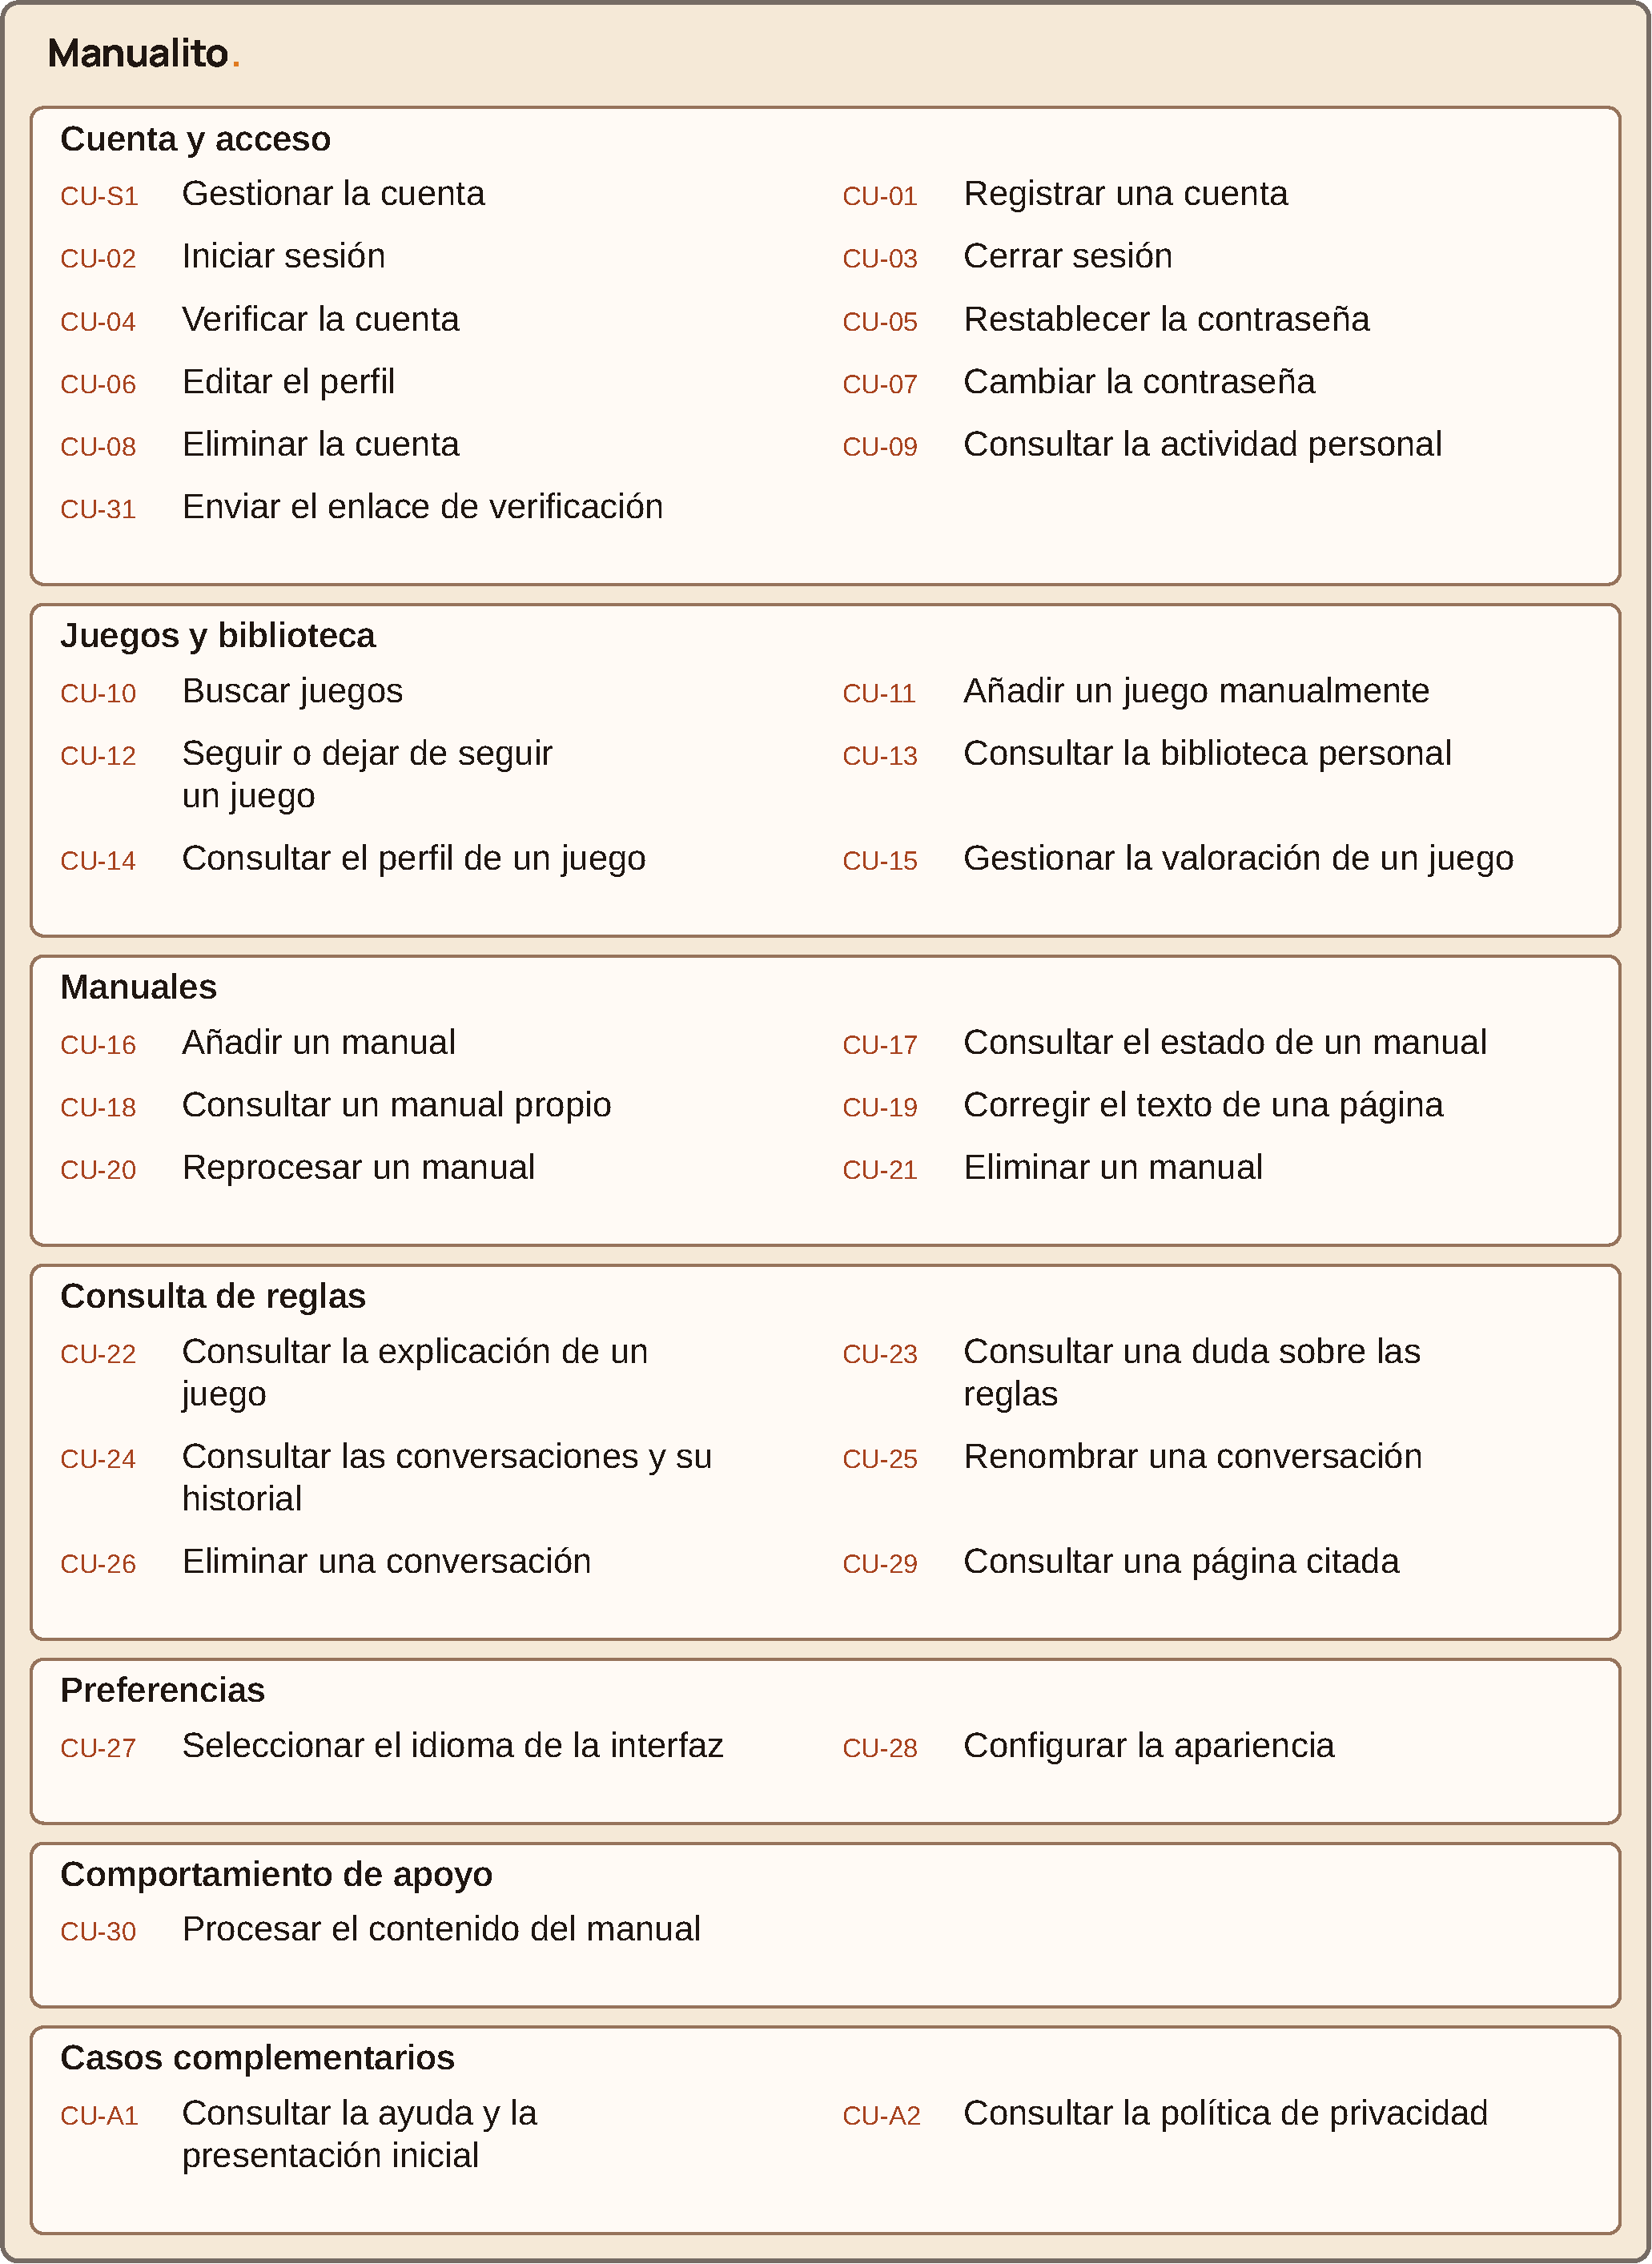
\includegraphics[width=\linewidth,height=0.88\textheight,keepaspectratio]{anexos/especificacion-de-requisitos/uml-general.pdf}
    \caption{Resumen de los casos de uso de \textit{Manualito}.}
    \label{fig:cu:general}
\end{figure}
\clearpage

\includepdf[
    pages=1,
    scale=0.94,
    offset=0 8,
    pagecommand={\thispagestyle{empty}\AddToShipoutPictureFG*{\AtPageLowerLeft{
        \put(0,20){\makebox[\paperwidth]{\parbox{0.9\paperwidth}{
            \captionFiguraCU{Diagrama general de casos de uso de \textit{Manualito}.}
            \label{fig:cu:global}
        }}}
    }}}
]{img/anexos/especificacion-de-requisitos/uml-global.pdf}

\subsection{Descripción de los casos de uso}

Cada uno de los casos de uso indica el autor, los actores, el objetivo, el inicio del caso,
las precondiciones, las acciones y el resultado esperado. Las alternativas
describen las decisiones y los errores que modifican la secuencia principal.

Esta organización permite comprobar el comportamiento y seguir su relación
con los requisitos, de acuerdo con la adaptación de
\acs{ISO}/\acs{IEC}/\acs{IEEE} 29148:2018 utilizada en el
proyecto~\cite{iso_29148_2018}.

\begingroup
\footnotesize
\setlength{\parskip}{0pt}
\SetTblrInner[longtblr]{measure=vbox,stretch=-1}
\SetTblrTemplate{conthead,contfoot,middlehead,lasthead}{empty}

\subsubsection{Cuenta y acceso}

% CU-S1
\begin{longtblr}[
    caption={\textbf{CU-S1}. Gestionar la cuenta.},
    label={tab:cu:CU-S1}
]{
    width=\linewidth,
    colspec={Q[l,wd=0.24\linewidth] X[l]},
    rows={valign=t},
    row{1}={bg=gray!18,font=\bfseries},
    column{1}={font=\bfseries},
    hline{1,Z}={0.8pt}, hline{2}={0.5pt},
    hborder{2-9,Y}={pagebreak=no},
    rowhead=1, leftsep=4pt, rightsep=4pt, rowsep=2.8pt
}
        CU-S1 & Gestionar la cuenta \\
        Autor & Ibai Moya Aroz \\
        Requisitos asociados & \refRequisito{RF-1.3}, \refRequisito{RF-1.4}, \refRequisito{RF-1.6}, \refRequisito{RF-1.7}, \refRequisito{RF-1.8}, \refRequisito{RF-1.9}, \refRequisito{RF-5.1}, \refRequisito{RF-5.2} \\
        Actores & Usuario. \\
        Descripción & El usuario consulta los datos y las opciones de su cuenta y decide si necesita realizar alguna operación. \\
        Inicio & El usuario abre el perfil, la sección de seguridad o los ajustes de su cuenta. \\
        Precondiciones & El usuario ha iniciado sesión. \\
        Acciones & \begin{pasosCU}
            \item El sistema muestra la información y las operaciones disponibles en la sección elegida.
            \item El usuario consulta los datos y decide si quiere realizar alguna de las operaciones disponibles.
            \item Si realiza una operación, el sistema muestra su resultado. El usuario puede continuar la gestión o terminarla.
        \end{pasosCU} \\
        Postcondiciones & El usuario ha consultado la información de su cuenta y los cambios aceptados quedan aplicados. Si cierra sesión o elimina la cuenta, la gestión termina mostrando el acceso público. \\
        Alternativas & \begin{alternativasCU}
            \item El usuario puede consultar la información y salir sin modificarla.
            \item Si cancela una operación o el sistema la rechaza, puede continuar la gestión sin dar por aplicado el cambio.
        \end{alternativasCU} \\
\end{longtblr}

\clearpage

% CU-01
\begin{longtblr}[
    caption={\textbf{CU-01}. Registrar una cuenta.},
    label={tab:cu:CU-01}
]{
    width=\linewidth,
    colspec={Q[l,wd=0.24\linewidth] X[l]},
    rows={valign=t},
    row{1}={bg=gray!18,font=\bfseries},
    column{1}={font=\bfseries},
    hline{1,Z}={0.8pt}, hline{2}={0.5pt},
    hborder{2-9,Y}={pagebreak=no},
    rowhead=1, leftsep=4pt, rightsep=4pt, rowsep=2.8pt
}
        CU-01 & Registrar una cuenta \\
        Autor & Ibai Moya Aroz \\
        Requisitos asociados & \refRequisito{RF-1.1} \\
        Actores & Usuario. \\
        Descripción & El usuario crea una cuenta para acceder a las funciones de \textit{Manualito} que requieren identificación. \\
        Inicio & El usuario selecciona la opción de crear una cuenta. \\
        Precondiciones & El usuario no ha iniciado sesión y dispone de un correo electrónico al que puede acceder. \\
        Acciones & \begin{pasosCU}
            \item El usuario introduce su nombre de usuario, correo electrónico y contraseña, y confirma esta última.
            \item Acepta la política de privacidad y solicita crear la cuenta.
            \item El sistema valida los datos, crea la cuenta e inicia la sesión.
            \item Mediante \refCasoUso{CU-31}, el sistema encarga el envío del enlace de verificación. El registro termina y el usuario puede acceder a la aplicación.
        \end{pasosCU} \\
        Postcondiciones & La cuenta queda creada y la sesión iniciada, con la verificación pendiente. El usuario puede verificarla después mediante \refCasoUso{CU-04}. \\
        Alternativas & \begin{alternativasCU}
            \item Si los datos no son válidos, el nombre o el correo ya están registrados, o falta la aceptación de la política, no se completa el registro.
            \item Si falla la entrega del correo, la cuenta sigue pendiente de verificación. El usuario puede solicitar otro envío mediante \refCasoUso{CU-31}.
        \end{alternativasCU} \\
\end{longtblr}

\clearpage

% CU-02
\begin{longtblr}[
    caption={\textbf{CU-02}. Iniciar sesión.},
    label={tab:cu:CU-02}
]{
    width=\linewidth,
    colspec={Q[l,wd=0.24\linewidth] X[l]},
    rows={valign=t},
    row{1}={bg=gray!18,font=\bfseries},
    column{1}={font=\bfseries},
    hline{1,Z}={0.8pt}, hline{2}={0.5pt},
    hborder{2-9,Y}={pagebreak=no},
    rowhead=1, leftsep=4pt, rightsep=4pt, rowsep=2.8pt
}
        CU-02 & Iniciar sesión \\
        Autor & Ibai Moya Aroz \\
        Requisitos asociados & \refRequisito{RF-1.2} \\
        Actores & Usuario. \\
        Descripción & El usuario accede a su cuenta mediante sus credenciales. \\
        Inicio & El usuario abre el formulario de acceso a su cuenta. \\
        Precondiciones & El usuario tiene una cuenta activa y no ha iniciado sesión. \\
        Acciones & \begin{pasosCU}
            \item El usuario introduce su correo electrónico o nombre de usuario y su contraseña.
            \item Solicita iniciar sesión y el sistema comprueba las credenciales.
            \item Si son válidas, el sistema inicia la sesión y permite acceder a las funciones de la cuenta.
        \end{pasosCU} \\
        Postcondiciones & El usuario queda identificado y puede utilizar las funciones que requieren una sesión iniciada. \\
        Alternativas & \begin{alternativasCU}
            \item Si las credenciales no son válidas, el sistema rechaza el acceso y el usuario puede corregirlas o abandonar el intento.
            \item La falta de verificación de la cuenta no impide iniciar sesión.
        \end{alternativasCU} \\
\end{longtblr}

\clearpage

% CU-03
\begin{longtblr}[
    caption={\textbf{CU-03}. Cerrar sesión.},
    label={tab:cu:CU-03}
]{
    width=\linewidth,
    colspec={Q[l,wd=0.24\linewidth] X[l]},
    rows={valign=t},
    row{1}={bg=gray!18,font=\bfseries},
    column{1}={font=\bfseries},
    hline{1,Z}={0.8pt}, hline{2}={0.5pt},
    hborder{2-9,Y}={pagebreak=no},
    rowhead=1, leftsep=4pt, rightsep=4pt, rowsep=2.8pt
}
        CU-03 & Cerrar sesión \\
        Autor & Ibai Moya Aroz \\
        Requisitos asociados & \refRequisito{RF-1.3} \\
        Actores & Usuario. \\
        Descripción & El usuario cierra la sesión que está utilizando. \\
        Inicio & El usuario solicita cerrar la sesión desde el perfil o los ajustes. \\
        Precondiciones & El usuario ha iniciado sesión. \\
        Acciones & \begin{pasosCU}
            \item El sistema revoca la sesión.
            \item El sistema muestra el acceso público.
        \end{pasosCU} \\
        Postcondiciones & La sesión cerrada deja de permitir el acceso a las funciones protegidas. Para volver a utilizarlas, el usuario debe iniciar sesión. \\
        Alternativas & Si la sesión ya ha caducado, el usuario permanece en el acceso público. \\
\end{longtblr}

\clearpage

% CU-04
\begin{longtblr}[
    caption={\textbf{CU-04}. Verificar la cuenta.},
    label={tab:cu:CU-04}
]{
    width=\linewidth,
    colspec={Q[l,wd=0.24\linewidth] X[l]},
    rows={valign=t},
    row{1}={bg=gray!18,font=\bfseries},
    column{1}={font=\bfseries},
    hline{1,Z}={0.8pt}, hline{2}={0.5pt},
    hborder{2-9,Y}={pagebreak=no},
    rowhead=1, leftsep=4pt, rightsep=4pt, rowsep=2.8pt
}
        CU-04 & Verificar la cuenta \\
        Autor & Ibai Moya Aroz \\
        Requisitos asociados & \refRequisito{RF-1.4} \\
        Actores & Usuario. \\
        Descripción & El usuario confirma que tiene acceso al correo electrónico asociado a su cuenta. \\
        Inicio & El usuario abre el enlace de verificación recibido por correo. \\
        Precondiciones & La cuenta está activa y el usuario ha recibido un enlace de verificación. No necesita haber iniciado sesión. \\
        Acciones & \begin{pasosCU}
            \item El sistema comprueba que el enlace permite verificar la cuenta.
            \item Marca la cuenta como verificada e invalida el enlace utilizado.
            \item El sistema muestra el resultado de la verificación.
        \end{pasosCU} \\
        Postcondiciones & La cuenta queda verificada y el enlace no permite una nueva verificación. \\
        Alternativas & \begin{alternativasCU}
            \item El sistema rechaza los enlaces que no reconoce. Si la cuenta sigue pendiente de verificación, también rechaza los enlaces caducados o utilizados.
            \item Si la cuenta ya está verificada y el sistema reconoce el enlace, conserva ese estado.
            \item Si necesita otro enlace, el usuario puede solicitarlo mediante \refCasoUso{CU-31}.
        \end{alternativasCU} \\
\end{longtblr}

\clearpage

% CU-05
\begin{longtblr}[
    caption={\textbf{CU-05}. Restablecer la contraseña.},
    label={tab:cu:CU-05}
]{
    width=\linewidth,
    colspec={Q[l,wd=0.24\linewidth] X[l]},
    rows={valign=t},
    row{1}={bg=gray!18,font=\bfseries},
    column{1}={font=\bfseries},
    hline{1,Z}={0.8pt}, hline{2}={0.5pt},
    hborder{2-9,Y}={pagebreak=no},
    rowhead=1, leftsep=4pt, rightsep=4pt, rowsep=2.8pt
}
        CU-05 & Restablecer la contraseña \\
        Autor & Ibai Moya Aroz \\
        Requisitos asociados & \refRequisito{RF-1.5} \\
        Actores & Usuario, Servicio de correo. \\
        Descripción & El usuario recupera el acceso a su cuenta cuando no recuerda la contraseña. \\
        Inicio & El usuario selecciona la opción de restablecer una contraseña olvidada. \\
        Precondiciones & La cuenta está activa y el usuario tiene acceso a su correo electrónico. \\
        Acciones & \begin{pasosCU}
            \item El usuario solicita restablecer la contraseña e indica el correo electrónico de su cuenta.
            \item El sistema genera un enlace de un solo uso y encarga su envío al servicio de correo.
            \item El usuario abre el enlace recibido e introduce y confirma una nueva contraseña.
            \item El sistema valida el enlace y la contraseña, guarda el cambio, invalida el enlace y revoca las sesiones anteriores.
            \item El sistema confirma el cambio y permite volver al formulario de acceso.
        \end{pasosCU} \\
        Postcondiciones & La contraseña queda actualizada y el correo queda verificado si todavía no lo estaba. El enlace utilizado y las sesiones anteriores dejan de ser válidos. \\
        Alternativas & \begin{alternativasCU}
            \item La respuesta a la solicitud no revela si el correo electrónico está registrado.
            \item Si el enlace no es válido, ha caducado o ya se ha utilizado, el sistema rechaza el restablecimiento.
            \item Si la nueva contraseña no cumple las condiciones o su confirmación no coincide, el usuario debe corregirla antes de continuar.
        \end{alternativasCU} \\
\end{longtblr}


\clearpage

% CU-06
\begin{longtblr}[
    caption={\textbf{CU-06}. Editar el perfil.},
    label={tab:cu:CU-06}
]{
    width=\linewidth,
    colspec={Q[l,wd=0.24\linewidth] X[l]},
    rows={valign=t},
    row{1}={bg=gray!18,font=\bfseries},
    column{1}={font=\bfseries},
    hline{1,Z}={0.8pt}, hline{2}={0.5pt},
    hborder{2-9,Y}={pagebreak=no},
    rowhead=1, leftsep=4pt, rightsep=4pt, rowsep=2.8pt
}
        CU-06 & Editar el perfil \\
        Autor & Ibai Moya Aroz \\
        Requisitos asociados & \refRequisito{RF-1.6} \\
        Actores & Usuario. \\
        Descripción & El usuario actualiza los datos con los que se identifica en su cuenta. \\
        Inicio & El usuario abre la edición del perfil desde su cuenta. \\
        Precondiciones & El usuario ha iniciado sesión. \\
        Acciones & \begin{pasosCU}
            \item El usuario modifica el nombre de usuario, el correo electrónico o la imagen de perfil.
            \item Solicita guardar los cambios y el sistema comprueba los datos modificados.
            \item El sistema guarda los cambios aceptados y muestra el perfil actualizado.
        \end{pasosCU} \\
        Postcondiciones & El perfil muestra los cambios guardados. Si se ha modificado el correo electrónico, la cuenta queda pendiente de verificarlo. \\
        Alternativas & \begin{alternativasCU}
            \item El usuario puede cancelar la edición sin guardar los cambios.
            \item Si algún dato no es válido o el nombre o el correo ya están registrados, el sistema rechaza el cambio y permite corregirlo.
        \end{alternativasCU} \\
\end{longtblr}

\clearpage

% CU-07
\begin{longtblr}[
    caption={\textbf{CU-07}. Cambiar la contraseña.},
    label={tab:cu:CU-07}
]{
    width=\linewidth,
    colspec={Q[l,wd=0.24\linewidth] X[l]},
    rows={valign=t},
    row{1}={bg=gray!18,font=\bfseries},
    column{1}={font=\bfseries},
    hline{1,Z}={0.8pt}, hline{2}={0.5pt},
    hborder{2-9,Y}={pagebreak=no},
    rowhead=1, leftsep=4pt, rightsep=4pt, rowsep=2.8pt
}
        CU-07 & Cambiar la contraseña \\
        Autor & Ibai Moya Aroz \\
        Requisitos asociados & \refRequisito{RF-1.7} \\
        Actores & Usuario. \\
        Descripción & El usuario sustituye la contraseña de su cuenta y conserva la sesión desde la que realiza el cambio. \\
        Inicio & El usuario accede a la sección de seguridad para cambiar la contraseña. \\
        Precondiciones & El usuario ha iniciado sesión y conoce su contraseña actual. \\
        Acciones & \begin{pasosCU}
            \item El usuario introduce la contraseña actual y la nueva, que debe confirmar.
            \item Solicita el cambio y el sistema comprueba la contraseña actual y valida la nueva.
            \item El sistema guarda la nueva contraseña, revoca las demás sesiones y confirma el cambio.
        \end{pasosCU} \\
        Postcondiciones & La contraseña queda actualizada y solo permanece activa la sesión desde la que se ha realizado el cambio. \\
        Alternativas & Si la contraseña actual es incorrecta, la nueva no cumple las condiciones o su confirmación no coincide, el sistema impide el cambio. \\
\end{longtblr}

\clearpage

% CU-08
\begin{longtblr}[
    caption={\textbf{CU-08}. Eliminar la cuenta.},
    label={tab:cu:CU-08}
]{
    width=\linewidth,
    colspec={Q[l,wd=0.24\linewidth] X[l]},
    rows={valign=t},
    row{1}={bg=gray!18,font=\bfseries},
    column{1}={font=\bfseries},
    hline{1,Z}={0.8pt}, hline{2}={0.5pt},
    hborder{2-9,Y}={pagebreak=no},
    rowhead=1, leftsep=4pt, rightsep=4pt, rowsep=2.8pt
}
        CU-08 & Eliminar la cuenta \\
        Autor & Ibai Moya Aroz \\
        Requisitos asociados & \refRequisito{RF-1.8} \\
        Actores & Usuario. \\
        Descripción & El usuario elimina su cuenta y retira el acceso a la información asociada a ella. \\
        Inicio & El usuario solicita eliminar su cuenta desde los ajustes o la sección de seguridad. \\
        Precondiciones & El usuario ha iniciado sesión en la cuenta que desea eliminar. \\
        Acciones & \begin{pasosCU}
            \item El usuario revisa la información que dejará de estar disponible e introduce su nombre de usuario para confirmar el borrado.
            \item El sistema comprueba la confirmación, revoca las sesiones y hace inaccesibles la cuenta y sus recursos.
            \item El sistema inicia la limpieza de los recursos asociados y muestra el acceso público.
        \end{pasosCU} \\
        Postcondiciones & La cuenta, los manuales, las conversaciones y las valoraciones asociadas dejan de ser accesibles, y sus sesiones dejan de ser válidas. \\
        Alternativas & \begin{alternativasCU}
            \item El usuario puede cancelar antes de confirmar el borrado y continuar utilizando la cuenta.
            \item Si el nombre introducido no coincide con el de la cuenta, el sistema impide la eliminación.
            \item Si la solicitud falla, el sistema informa del error sin confirmar que la cuenta se haya eliminado.
        \end{alternativasCU} \\
\end{longtblr}

\clearpage

% CU-09
\begin{longtblr}[
    caption={\textbf{CU-09}. Consultar la actividad personal.},
    label={tab:cu:CU-09}
]{
    width=\linewidth,
    colspec={Q[l,wd=0.24\linewidth] X[l]},
    rows={valign=t},
    row{1}={bg=gray!18,font=\bfseries},
    column{1}={font=\bfseries},
    hline{1,Z}={0.8pt}, hline{2}={0.5pt},
    hborder{2-9,Y}={pagebreak=no},
    rowhead=1, leftsep=4pt, rightsep=4pt, rowsep=2.8pt
}
        CU-09 & Consultar la actividad personal \\
        Autor & Ibai Moya Aroz \\
        Requisitos asociados & \refRequisito{RF-1.9} \\
        Actores & Usuario. \\
        Descripción & El usuario consulta un resumen de la actividad que ha realizado con su cuenta. \\
        Inicio & El usuario abre su perfil para consultar la actividad personal. \\
        Precondiciones & El usuario ha iniciado sesión. \\
        Acciones & \begin{pasosCU}
            \item El sistema obtiene los recuentos de actividad de la cuenta.
            \item El sistema muestra, junto a los datos del perfil, el número de juegos con actividad, manuales subidos y conversaciones creadas.
        \end{pasosCU} \\
        Postcondiciones & El usuario ha consultado los recuentos de su actividad personal. \\
        Alternativas & Si no hay actividad de alguno de estos tipos, su recuento es cero. \\
\end{longtblr}

\clearpage

% CU-31
\begin{longtblr}[
    caption={\textbf{CU-31}. Enviar el enlace de verificación.},
    label={tab:cu:CU-31}
]{
    width=\linewidth,
    colspec={Q[l,wd=0.24\linewidth] X[l]},
    rows={valign=t},
    row{1}={bg=gray!18,font=\bfseries},
    column{1}={font=\bfseries},
    hline{1,Z}={0.8pt}, hline{2}={0.5pt},
    hborder{2-9,Y}={pagebreak=no},
    rowhead=1, leftsep=4pt, rightsep=4pt, rowsep=2.8pt
}
        CU-31 & Enviar el enlace de verificación \\
        Autor & Ibai Moya Aroz \\
        Requisitos asociados & \refRequisito{RF-1.4} \\
        Actores & Usuario, Servicio de correo. \\
        Descripción & El sistema proporciona un enlace para que el usuario pueda verificar su cuenta. \\
        Inicio & Se crea una cuenta, se cambia su correo o el usuario solicita otro enlace de verificación. \\
        Precondiciones & La cuenta está activa y su correo está pendiente de verificación. \\
        Acciones & \begin{pasosCU}
            \item El sistema obtiene el correo de destino y comprueba que procede emitir un enlace.
            \item Genera un enlace de verificación vigente e invalida los anteriores cuando los haya.
            \item Encarga el envío al servicio de correo y continúa la operación que lo solicitó o responde a la petición de reenvío.
        \end{pasosCU} \\
        Postcondiciones & Se emite un enlace y se encarga su envío. La cuenta sigue pendiente de verificación hasta que el usuario utilice un enlace válido en \refCasoUso{CU-04}. \\
        Alternativas & \begin{alternativasCU}
            \item La respuesta a una solicitud pública no revela si existe una cuenta con ese correo.
            \item Si la cuenta ya está verificada, no está activa o no ha transcurrido la espera entre solicitudes, no se emite otro enlace.
            \item Si falla la entrega, la cuenta conserva la verificación pendiente.
        \end{alternativasCU} \\
\end{longtblr}

\clearpage

\subsubsection{Juegos y biblioteca}

% CU-10
\begin{longtblr}[
    caption={\textbf{CU-10}. Buscar juegos.},
    label={tab:cu:CU-10}
]{
    width=\linewidth,
    colspec={Q[l,wd=0.24\linewidth] X[l]},
    rows={valign=t},
    row{1}={bg=gray!18,font=\bfseries},
    column{1}={font=\bfseries},
    hline{1,Z}={0.8pt}, hline{2}={0.5pt},
    hborder{2-9,Y}={pagebreak=no},
    rowhead=1, leftsep=4pt, rightsep=4pt, rowsep=2.8pt
}
        CU-10 & Buscar juegos \\
        Autor & Ibai Moya Aroz \\
        Requisitos asociados & \refRequisito{RF-2.1} \\
        Actores & Usuario, Catálogo externo de juegos. \\
        Descripción & Permite localizar un juego por su nombre para conocerlo o asociarle un manual. \\
        Inicio & El usuario abre la búsqueda durante la exploración o al añadir un manual. \\
        Precondiciones & El usuario ha iniciado sesión. \\
        Acciones & \begin{pasosCU}
            \item El usuario introduce el nombre del juego que busca.
            \item El sistema busca coincidencias y muestra los resultados.
            \item El usuario puede seleccionar un resultado para consultar el juego durante la exploración o para continuar añadiendo un manual.
        \end{pasosCU} \\
        Postcondiciones & El sistema muestra los resultados de la búsqueda o indica que no hay coincidencias. Si selecciona un juego durante una subida, ese juego queda elegido para asociarle el manual. \\
        Alternativas & \begin{alternativasCU}
            \item Si no hay coincidencias, el sistema lo indica y el usuario puede cambiar la búsqueda o terminarla.
            \item Durante la subida de un manual, una búsqueda sin coincidencias también permite añadir el juego manualmente.
        \end{alternativasCU} \\
\end{longtblr}

\clearpage

% CU-11
\begin{longtblr}[
    caption={\textbf{CU-11}. Añadir un juego manualmente.},
    label={tab:cu:CU-11}
]{
    width=\linewidth,
    colspec={Q[l,wd=0.24\linewidth] X[l]},
    rows={valign=t},
    row{1}={bg=gray!18,font=\bfseries},
    column{1}={font=\bfseries},
    hline{1,Z}={0.8pt}, hline{2}={0.5pt},
    hborder{2-9,Y}={pagebreak=no},
    rowhead=1, leftsep=4pt, rightsep=4pt, rowsep=2.8pt
}
        CU-11 & Añadir un juego manualmente \\
        Autor & Ibai Moya Aroz \\
        Requisitos asociados & \refRequisito{RF-2.2} \\
        Actores & Usuario. \\
        Descripción & Permite registrar un juego que no aparece en la búsqueda para poder asociarle el manual que se está añadiendo. \\
        Inicio & El usuario elige añadir el juego tras una búsqueda sin coincidencias. \\
        Precondiciones & El usuario ha iniciado sesión y la búsqueda de \refCasoUso{CU-10} no ha devuelto coincidencias durante \refCasoUso{CU-16}. \\
        Acciones & \begin{pasosCU}
            \item El usuario confirma el nombre del juego que quiere añadir.
            \item El sistema valida el nombre, registra el juego y lo selecciona para continuar la subida.
        \end{pasosCU} \\
        Postcondiciones & El juego queda registrado y seleccionado para asociarle el manual. \\
        Alternativas & \begin{alternativasCU}
            \item Si el nombre no es válido, el usuario debe corregirlo antes de añadir el juego.
            \item El usuario puede cancelar la creación y volver a buscar un juego existente.
        \end{alternativasCU} \\
\end{longtblr}

\clearpage

% CU-12
\begin{longtblr}[
    caption={\textbf{CU-12}. Seguir o dejar de seguir un juego.},
    label={tab:cu:CU-12}
]{
    width=\linewidth,
    colspec={Q[l,wd=0.24\linewidth] X[l]},
    rows={valign=t},
    row{1}={bg=gray!18,font=\bfseries},
    column{1}={font=\bfseries},
    hline{1,Z}={0.8pt}, hline{2}={0.5pt},
    hborder{2-9,Y}={pagebreak=no},
    rowhead=1, leftsep=4pt, rightsep=4pt, rowsep=2.8pt
}
        CU-12 & Seguir o dejar de seguir un juego \\
        Autor & Ibai Moya Aroz \\
        Requisitos asociados & \refRequisito{RF-2.3}, \refRequisito{RF-2.3.1} \\
        Actores & Usuario. \\
        Descripción & Permite decidir si un juego debe aparecer entre los juegos seguidos de la biblioteca personal. \\
        Inicio & El usuario decide seguir el juego que está consultando o dejar de seguirlo. \\
        Precondiciones & El usuario ha iniciado sesión y el juego existe. \\
        Acciones & \begin{pasosCU}
            \item Durante la consulta del perfil, el usuario elige seguir el juego o dejar de seguirlo.
            \item El sistema guarda la decisión, actualiza la biblioteca personal e indica si el usuario sigue el juego.
        \end{pasosCU} \\
        Postcondiciones & La decisión queda guardada y el perfil indica si el usuario sigue el juego. \\
        Alternativas & Si el usuario decide dejar de seguir el juego, una actividad posterior no vuelve a seguirlo automáticamente. \\
\end{longtblr}

\clearpage

% CU-13
\begin{longtblr}[
    caption={\textbf{CU-13}. Consultar la biblioteca personal.},
    label={tab:cu:CU-13}
]{
    width=\linewidth,
    colspec={Q[l,wd=0.24\linewidth] X[l]},
    rows={valign=t},
    row{1}={bg=gray!18,font=\bfseries},
    column{1}={font=\bfseries},
    hline{1,Z}={0.8pt}, hline{2}={0.5pt},
    hborder{2-9,Y}={pagebreak=no},
    rowhead=1, leftsep=4pt, rightsep=4pt, rowsep=2.8pt
}
        CU-13 & Consultar la biblioteca personal \\
        Autor & Ibai Moya Aroz \\
        Requisitos asociados & \refRequisito{RF-2.4}, \refRequisito{RF-2.4.1}, \refRequisito{RF-2.4.2} \\
        Actores & Usuario. \\
        Descripción & Permite localizar los juegos seguidos y los manuales propios y consultar la información de cada uno. \\
        Inicio & El usuario accede a la biblioteca personal. \\
        Precondiciones & El usuario ha iniciado sesión. \\
        Acciones & \begin{pasosCU}
            \item El usuario elige consultar los juegos o los manuales.
            \item El sistema muestra los juegos seguidos o los manuales propios.
            \item El usuario puede filtrar los manuales y el sistema muestra las coincidencias.
            \item El usuario puede seleccionar una entrada para consultar los detalles del juego, el contenido del manual o su estado de procesamiento.
        \end{pasosCU} \\
        Postcondiciones & La biblioteca muestra los juegos seguidos o los manuales propios según la selección y los filtros aplicados. Si el usuario elimina un manual, la lista deja de mostrarlo. \\
        Alternativas & \begin{alternativasCU}
            \item Si la lista está vacía o el filtro no devuelve resultados, el sistema lo indica.
            \item El usuario puede eliminar un manual propio durante la consulta. Tras confirmar la eliminación, la biblioteca muestra los manuales restantes o indica que no hay ninguno.
        \end{alternativasCU} \\
\end{longtblr}

\clearpage

% CU-14
\begin{longtblr}[
    caption={\textbf{CU-14}. Consultar el perfil de un juego.},
    label={tab:cu:CU-14}
]{
    width=\linewidth,
    colspec={Q[l,wd=0.24\linewidth] X[l]},
    rows={valign=t},
    row{1}={bg=gray!18,font=\bfseries},
    column{1}={font=\bfseries},
    hline{1,Z}={0.8pt}, hline{2}={0.5pt},
    hborder{2-9,Y}={pagebreak=no},
    rowhead=1, leftsep=4pt, rightsep=4pt, rowsep=2.8pt
}
        CU-14 & Consultar el perfil de un juego \\
        Autor & Ibai Moya Aroz \\
        Requisitos asociados & \refRequisito{RF-2.5} \\
        Actores & Usuario. \\
        Descripción & Permite conocer un juego, revisar la actividad personal asociada y ampliar la consulta mediante sus manuales y conversaciones. \\
        Inicio & El usuario selecciona un juego para consultar su perfil. \\
        Precondiciones & El usuario ha iniciado sesión y el juego existe. \\
        Acciones & \begin{pasosCU}
            \item El sistema muestra los datos del juego, los manuales accesibles, la valoración propia y el número de conversaciones del usuario, e indica si sigue el juego.
            \item El usuario consulta esta información y puede profundizar en las reglas, los manuales o las conversaciones antes de terminar.
        \end{pasosCU} \\
        Postcondiciones & El perfil refleja la información accesible y los cambios realizados durante la consulta. \\
        Alternativas & \begin{alternativasCU}
            \item Sin manuales utilizables no se generan explicaciones ni respuestas nuevas, pero el perfil sigue siendo consultable.
            \item Los manuales compartidos pueden aportar contenido para consultas y abrirse en el visor en modo de solo lectura.
        \end{alternativasCU} \\
\end{longtblr}

\clearpage

% CU-15
\begin{longtblr}[
    caption={\textbf{CU-15}. Gestionar la valoración de un juego.},
    label={tab:cu:CU-15}
]{
    width=\linewidth,
    colspec={Q[l,wd=0.24\linewidth] X[l]},
    rows={valign=t},
    row{1}={bg=gray!18,font=\bfseries},
    column{1}={font=\bfseries},
    hline{1,Z}={0.8pt}, hline{2}={0.5pt},
    hborder{2-9,Y}={pagebreak=no},
    rowhead=1, leftsep=4pt, rightsep=4pt, rowsep=2.8pt
}
        CU-15 & Gestionar la valoración de un juego \\
        Autor & Ibai Moya Aroz \\
        Requisitos asociados & \refRequisito{RF-2.6}, \refRequisito{RF-2.3.2} \\
        Actores & Usuario. \\
        Descripción & Permite conservar una valoración personal del juego mediante una puntuación y una nota opcional. \\
        Inicio & El usuario abre la opción de valoración del perfil del juego. \\
        Precondiciones & El usuario ha iniciado sesión y el juego existe. \\
        Acciones & \begin{pasosCU}
            \item Desde el perfil del juego, el usuario selecciona una puntuación de uno a cinco y puede añadir una nota.
            \item El usuario solicita guardar la valoración y el sistema la registra o actualiza.
            \item El perfil muestra la valoración guardada.
        \end{pasosCU} \\
        Postcondiciones & La valoración queda creada, modificada o eliminada y el perfil refleja el resultado. \\
        Alternativas & \begin{alternativasCU}
            \item Si ya existe una valoración, el usuario puede modificarla o confirmar su eliminación.
            \item El usuario puede cancelar sin guardar los cambios.
            \item Si la valoración es la primera actividad sobre el juego, el sistema lo sigue automáticamente cuando no existe una decisión explícita anterior.
        \end{alternativasCU} \\
\end{longtblr}

\clearpage

\subsubsection{Manuales}

% CU-16
\begin{longtblr}[
    caption={\textbf{CU-16}. Añadir un manual.},
    label={tab:cu:CU-16}
]{
    width=\linewidth,
    colspec={Q[l,wd=0.24\linewidth] X[l]},
    rows={valign=t},
    row{1}={bg=gray!18,font=\bfseries},
    column{1}={font=\bfseries},
    hline{1,Z}={0.8pt}, hline{2}={0.5pt},
    hborder{2-9,Y}={pagebreak=no},
    rowhead=1, leftsep=4pt, rightsep=4pt, rowsep=2.8pt
}
        CU-16 & Añadir un manual \\
        Autor & Ibai Moya Aroz \\
        Requisitos asociados & \refRequisito{RF-3.1}, \refRequisito{RF-3.2}, \refRequisito{RF-3.3}, \refRequisito{RF-3.10}, \refRequisito{RF-2.3.2} \\
        Actores & Usuario. \\
        Descripción & Permite asociar un manual a un juego y preparar su contenido para utilizarlo en las consultas. \\
        Inicio & El usuario solicita añadir un manual, desde el perfil de un juego o desde la opción de subida. \\
        Precondiciones & El usuario ha iniciado sesión y dispone del manual en un documento \acs{PDF} o en imágenes. \\
        Acciones & \begin{pasosCU}
            \item El usuario acepta el juego preseleccionado o selecciona uno.
            \item El usuario añade el documento o las imágenes y elige si el manual será privado o compartido. Si añade varias imágenes, puede revisarlas, ordenarlas y retirar las que no sean útiles.
            \item Si comparte el manual, elige si quiere mostrar su nombre. Por defecto aparece como \guillemotleft{}Anónimo\guillemotright{}.
            \item El usuario confirma la subida. El sistema valida los formatos, los tamaños y el número de páginas, y comprueba si el manual está duplicado.
            \item El sistema guarda la fuente aceptada y ejecuta \refCasoUso{CU-30} en segundo plano.
        \end{pasosCU} \\
        Postcondiciones & El manual aceptado queda asociado al juego con la visibilidad y la opción de mostrar el nombre elegidas, y el juego empieza a seguirse automáticamente cuando corresponde. Su contenido queda preparado para consultas si el procesamiento obtiene un resultado utilizable. En caso contrario, se registra el fallo o la ausencia de texto útil. \\
        Alternativas & \begin{alternativasCU}
            \item El usuario puede cancelar antes de enviar el manual.
            \item El sistema rechaza los archivos que incumplen los límites y los manuales duplicados antes de procesarlos.
            \item El usuario puede seguir utilizando la aplicación mientras se procesa el manual.
        \end{alternativasCU} \\
\end{longtblr}


\clearpage

% CU-17
\begin{longtblr}[
    caption={\textbf{CU-17}. Consultar el estado de un manual.},
    label={tab:cu:CU-17}
]{
    width=\linewidth,
    colspec={Q[l,wd=0.24\linewidth] X[l]},
    rows={valign=t},
    row{1}={bg=gray!18,font=\bfseries},
    column{1}={font=\bfseries},
    hline{1,Z}={0.8pt}, hline{2}={0.5pt},
    hborder{2-9,Y}={pagebreak=no},
    rowhead=1, leftsep=4pt, rightsep=4pt, rowsep=2.8pt
}
        CU-17 & Consultar el estado de un manual \\
        Autor & Ibai Moya Aroz \\
        Requisitos asociados & \refRequisito{RF-3.5} \\
        Actores & Usuario. \\
        Descripción & Permite conocer el avance del procesamiento de un manual y el resultado de cada página. \\
        Inicio & El usuario elige consultar el estado de uno de sus manuales. \\
        Precondiciones & El usuario ha iniciado sesión y el manual le pertenece. No es necesario que su procesamiento haya terminado. \\
        Acciones & \begin{pasosCU}
            \item El sistema muestra el estado guardado del manual y de sus páginas.
            \item El usuario revisa qué páginas siguen pendientes o en procesamiento y cuáles se han completado o han fallado.
        \end{pasosCU} \\
        Postcondiciones & El usuario conoce el estado guardado del manual y de sus páginas. \\
        Alternativas & \begin{alternativasCU}
            \item El usuario puede abandonar la consulta y revisar el estado más tarde.
            \item Los fallos y la ausencia de texto útil se muestran como estados distintos del contenido preparado para consultas.
        \end{alternativasCU} \\
\end{longtblr}

\clearpage

% CU-18
\begin{longtblr}[
    caption={\textbf{CU-18}. Consultar un manual.},
    label={tab:cu:CU-18}
]{
    width=\linewidth,
    colspec={Q[l,wd=0.24\linewidth] X[l]},
    rows={valign=t},
    row{1}={bg=gray!18,font=\bfseries},
    column{1}={font=\bfseries},
    hline{1,Z}={0.8pt}, hline{2}={0.5pt},
    hborder{2-9,Y}={pagebreak=no},
    rowhead=1, leftsep=4pt, rightsep=4pt, rowsep=2.8pt
}
        CU-18 & Consultar un manual \\
        Autor & Ibai Moya Aroz \\
        Requisitos asociados & \refRequisito{RF-3.6}, \refRequisito{RF-3.6.1}, \refRequisito{RF-3.6.2}, \refRequisito{RF-3.6.3}, \refRequisito{RF-3.10} \\
        Actores & Usuario. \\
        Descripción & Permite leer un manual propio o compartido y contrastar el texto de cada página con su imagen. La información de procesamiento solo se muestra al propietario. \\
        Inicio & El usuario selecciona un manual disponible o una referencia a una de sus páginas. \\
        Precondiciones & El usuario ha iniciado sesión. El manual no está eliminado y le pertenece o está compartido. \\
        Acciones & \begin{pasosCU}
            \item El sistema abre el manual en la página indicada. Si no se ha indicado ninguna o esa página no existe, abre la primera página disponible.
            \item El sistema muestra el texto extraído o corregido y la imagen disponible. Si el manual es propio, también muestra los datos de origen, confianza y reutilización de la página.
            \item El usuario puede navegar entre las páginas o buscar texto y desplazarse entre las coincidencias.
        \end{pasosCU} \\
        Postcondiciones & El usuario consulta las páginas elegidas. Si el manual pertenece a otra cuenta, no puede editarlo, reprocesarlo, eliminarlo ni cambiar sus opciones. \\
        Alternativas & \begin{alternativasCU}
            \item Si la búsqueda no devuelve coincidencias o falta información de procesamiento, el sistema lo indica.
            \item Si el manual está compartido, el propietario puede cambiar la opción de mostrar su nombre y confirmar la elección. El sistema la guarda y la aplica al manual y a las fuentes de las respuestas.
            \item Si cancela la confirmación o falla el guardado, se conserva la opción anterior.
        \end{alternativasCU} \\
\end{longtblr}

\clearpage

% CU-19
\begin{longtblr}[
    caption={\textbf{CU-19}. Corregir el texto de una página.},
    label={tab:cu:CU-19}
]{
    width=\linewidth,
    colspec={Q[l,wd=0.24\linewidth] X[l]},
    rows={valign=t},
    row{1}={bg=gray!18,font=\bfseries},
    column{1}={font=\bfseries},
    hline{1,Z}={0.8pt}, hline{2}={0.5pt},
    hborder{2-9,Y}={pagebreak=no},
    rowhead=1, leftsep=4pt, rightsep=4pt, rowsep=2.8pt
}
        CU-19 & Corregir el texto de una página \\
        Autor & Ibai Moya Aroz \\
        Requisitos asociados & \refRequisito{RF-3.7} \\
        Actores & Usuario. \\
        Descripción & Permite corregir errores o completar el texto de una página para utilizar la versión revisada en las consultas. \\
        Inicio & El usuario solicita editar el texto de la página que está consultando. \\
        Precondiciones & El usuario ha iniciado sesión, la página existe y el manual es propio, privado y no se está procesando. \\
        Acciones & \begin{pasosCU}
            \item El usuario modifica el texto de la página que está consultando y confirma el cambio.
            \item El sistema guarda la corrección y solicita actualizar el contenido indexado de esa página.
            \item El visor muestra el texto corregido para continuar la lectura.
        \end{pasosCU} \\
        Postcondiciones & El texto corregido queda guardado y se solicita su actualización para las consultas. El texto de las demás páginas se conserva. \\
        Alternativas & \begin{alternativasCU}
            \item El usuario puede cancelar sin guardar o añadir texto a una página que todavía no lo tenga.
            \item El sistema rechaza la edición de un manual ajeno, compartido o que se esté procesando.
            \item Si falla la solicitud de actualización del contenido indexado después de guardar, el texto corregido se conserva y el sistema informa del error.
        \end{alternativasCU} \\
\end{longtblr}


\clearpage

% CU-20
\begin{longtblr}[
    caption={\textbf{CU-20}. Reprocesar un manual.},
    label={tab:cu:CU-20}
]{
    width=\linewidth,
    colspec={Q[l,wd=0.24\linewidth] X[l]},
    rows={valign=t},
    row{1}={bg=gray!18,font=\bfseries},
    column{1}={font=\bfseries},
    hline{1,Z}={0.8pt}, hline{2}={0.5pt},
    hborder{2-9,Y}={pagebreak=no},
    rowhead=1, leftsep=4pt, rightsep=4pt, rowsep=2.8pt
}
        CU-20 & Reprocesar un manual \\
        Autor & Ibai Moya Aroz \\
        Requisitos asociados & \refRequisito{RF-3.8}, \refRequisito{RF-3.8.1}, \refRequisito{RF-3.8.2} \\
        Actores & Usuario. \\
        Descripción & Permite obtener de nuevo el contenido de un manual completo o de una página a partir de las fuentes guardadas. \\
        Inicio & El usuario solicita repetir el procesamiento desde el visor del manual. \\
        Precondiciones & El usuario ha iniciado sesión, el manual le pertenece, conserva sus fuentes y su estado permite repetir el procesamiento. \\
        Acciones & \begin{pasosCU}
            \item El usuario elige reprocesar el manual completo o una página y confirma la operación.
            \item El sistema ejecuta \refCasoUso{CU-30} en segundo plano sobre las páginas seleccionadas.
            \item El sistema guarda el nuevo resultado o el fallo y actualiza el estado del manual y de las páginas afectadas.
        \end{pasosCU} \\
        Postcondiciones & El nuevo resultado o el fallo queda registrado. Si se reprocesa una sola página, se conserva el resto del manual. \\
        Alternativas & \begin{alternativasCU}
            \item El usuario puede cancelar antes de confirmar la operación.
            \item Si el estado del manual impide reprocesarlo, el sistema rechaza la solicitud.
            \item El reprocesamiento puede sustituir las correcciones manuales y puede terminar con un error. No requiere que el procesamiento anterior haya fallado.
        \end{alternativasCU} \\
\end{longtblr}

\clearpage

% CU-21
\begin{longtblr}[
    caption={\textbf{CU-21}. Eliminar un manual.},
    label={tab:cu:CU-21}
]{
    width=\linewidth,
    colspec={Q[l,wd=0.24\linewidth] X[l]},
    rows={valign=t},
    row{1}={bg=gray!18,font=\bfseries},
    column{1}={font=\bfseries},
    hline{1,Z}={0.8pt}, hline{2}={0.5pt},
    hborder{2-9,Y}={pagebreak=no},
    rowhead=1, leftsep=4pt, rightsep=4pt, rowsep=2.8pt
}
        CU-21 & Eliminar un manual \\
        Autor & Ibai Moya Aroz \\
        Requisitos asociados & \refRequisito{RF-3.9} \\
        Actores & Usuario. \\
        Descripción & Permite retirar un manual propio y su contenido del acceso del usuario. \\
        Inicio & El usuario solicita eliminar un manual desde la biblioteca o desde su visor. \\
        Precondiciones & El usuario ha iniciado sesión. El manual le pertenece y no está eliminado. No es necesario que su procesamiento haya terminado. \\
        Acciones & \begin{pasosCU}
            \item El usuario confirma la eliminación del manual.
            \item El sistema retira el acceso al manual y sus páginas y solicita la limpieza de sus archivos y del contenido indexado.
            \item Si la eliminación se inició en la biblioteca, el sistema actualiza la lista. Si se inició en el visor, termina la consulta del manual y muestra la biblioteca.
        \end{pasosCU} \\
        Postcondiciones & El manual y sus páginas dejan de ser accesibles y se solicita la limpieza de sus recursos. El historial de conversaciones se conserva. \\
        Alternativas & \begin{alternativasCU}
            \item El usuario puede cancelar sin eliminar el manual.
            \item Si se elimina la última fuente utilizable de un juego, las conversaciones existentes se conservan y quedan en modo de solo lectura.
        \end{alternativasCU} \\
\end{longtblr}

\clearpage

% CU-30
\begin{longtblr}[
    caption={\textbf{CU-30}. Procesar el contenido del manual.},
    label={tab:cu:CU-30}
]{
    width=\linewidth,
    colspec={Q[l,wd=0.24\linewidth] X[l]},
    rows={valign=t},
    row{1}={bg=gray!18,font=\bfseries},
    column{1}={font=\bfseries},
    hline{1,Z}={0.8pt}, hline{2}={0.5pt},
    hborder{2-9,Y}={pagebreak=no},
    rowhead=1, leftsep=4pt, rightsep=4pt, rowsep=2.8pt
}
        CU-30 & Procesar el contenido del manual \\
        Autor & Ibai Moya Aroz \\
        Requisitos asociados & \refRequisito{RF-3.4}, \refRequisito{RF-3.4.1}, \refRequisito{RF-3.4.2}, \refRequisito{RF-3.4.3}, \refRequisito{RF-3.4.4}, \refRequisito{RF-3.4.5} \\
        Actores & Usuario. \\
        Descripción & Prepara el texto del manual para que pueda recuperarse al generar explicaciones y responder preguntas sobre el juego. \\
        Inicio & El sistema inicia el procesamiento previsto en \refCasoUso{CU-16} o en \refCasoUso{CU-20}. \\
        Precondiciones & Las fuentes están guardadas y las páginas que deben procesarse están identificadas. \\
        Acciones & \begin{pasosCU}
            \item El sistema utiliza el texto del documento cuando es aprovechable. En caso contrario, preprocesa las imágenes y extrae su texto mediante \ac{OCR}.
            \item El sistema aplica el posprocesado y guarda el texto resultante.
            \item El sistema divide el texto en fragmentos y los indexa para recuperarlos durante las consultas.
            \item El sistema actualiza el estado del manual y de sus páginas según el resultado del procesamiento.
        \end{pasosCU} \\
        Postcondiciones & El contenido utilizable queda preparado para las consultas. Cuando el procesamiento falla o no obtiene texto útil, el estado del manual y de sus páginas refleja esa situación. \\
        Alternativas & \begin{alternativasCU}
            \item Si encuentra una página idéntica ya procesada, el sistema reutiliza su resultado sin repetir la extracción ni el posprocesado.
            \item Si falla una etapa o no se obtiene texto útil, el sistema registra el estado correspondiente.
        \end{alternativasCU} \\
\end{longtblr}

\clearpage

\subsubsection{Consulta de reglas}

% CU-22
\begin{longtblr}[
    caption={\textbf{CU-22}. Consultar la explicación de un juego.},
    label={tab:cu:CU-22}
]{
    width=\linewidth,
    colspec={Q[l,wd=0.24\linewidth] X[l]},
    rows={valign=t},
    row{1}={bg=gray!18,font=\bfseries},
    column{1}={font=\bfseries},
    hline{1,Z}={0.8pt}, hline{2}={0.5pt},
    hborder{2-9,Y}={pagebreak=no},
    rowhead=1, leftsep=4pt, rightsep=4pt, rowsep=2.8pt
}
        CU-22 & Consultar la explicación de un juego \\
        Autor & Ibai Moya Aroz \\
        Requisitos asociados & \refRequisito{RF-4.1} \\
        Actores & Usuario. \\
        Descripción & Permite conocer la preparación, el desarrollo y las condiciones de victoria de un juego a partir de sus manuales. \\
        Inicio & El usuario abre el perfil de un juego con manuales utilizables. \\
        Precondiciones & El usuario ha iniciado sesión y el juego dispone de manuales que puede utilizar para las consultas. \\
        Acciones & \begin{pasosCU}
            \item El sistema solicita automáticamente la explicación del juego.
            \item El sistema recupera la explicación conservada si sus fuentes no han cambiado. Si no dispone de una explicación vigente, la genera en segundo plano.
            \item El usuario consulta los apartados de la explicación a medida que están disponibles.
        \end{pasosCU} \\
        Postcondiciones & La explicación generada puede leerse desde el perfil del juego y se conserva para consultas posteriores mientras no cambien sus fuentes. \\
        Alternativas & \begin{alternativasCU}
            \item Si no hay manuales utilizables, se informa de que faltan fuentes y no se genera la explicación.
            \item Si la generación falla antes de obtener contenido, el sistema informa del error. Si ya hay apartados disponibles, conserva su contenido. El resto del perfil sigue disponible.
        \end{alternativasCU} \\
\end{longtblr}

\clearpage

% CU-23
\begin{longtblr}[
    caption={\textbf{CU-23}. Consultar una duda sobre las reglas.},
    label={tab:cu:CU-23}
]{
    width=\linewidth,
    colspec={Q[l,wd=0.24\linewidth] X[l]},
    rows={valign=t},
    row{1}={bg=gray!18,font=\bfseries},
    column{1}={font=\bfseries},
    hline{1,Z}={0.8pt}, hline{2}={0.5pt},
    hborder{2-9,Y}={pagebreak=no},
    rowhead=1, leftsep=4pt, rightsep=4pt, rowsep=2.8pt
}
        CU-23 & Consultar una duda sobre las reglas \\
        Autor & Ibai Moya Aroz \\
        Requisitos asociados & \refRequisito{RF-4.2.1}, \refRequisito{RF-4.3}, \refRequisito{RF-4.4}, \refRequisito{RF-4.5}, \refRequisito{RF-4.6}, \refRequisito{RF-4.7}, \refRequisito{RF-4.8}, \refRequisito{RF-2.3.2} \\
        Actores & Usuario. \\
        Descripción & Permite aclarar una duda sobre las reglas de un juego y contrastar la respuesta con los manuales utilizados. \\
        Inicio & El usuario envía una pregunta sobre las reglas del juego. \\
        Precondiciones & El usuario ha iniciado sesión y el juego dispone de fuentes utilizables. Si continúa una conversación, esta pertenece a su cuenta. \\
        Acciones & \begin{pasosCU}
            \item El sistema utiliza la conversación seleccionada o crea una nueva asociada al juego.
            \item El sistema guarda la pregunta y muestra la respuesta como pendiente. Si es el primer mensaje, asigna un título a la conversación a partir de su contenido.
            \item El sistema genera la respuesta en segundo plano a partir de los manuales utilizables. Si hay mensajes anteriores, los tiene en cuenta para interpretar la pregunta.
            \item El sistema muestra la respuesta en español o inglés según el idioma detectado en el turno, junto con las referencias utilizadas.
            \item El usuario lee la respuesta y puede contrastarla consultando una página citada mediante \refCasoUso{CU-29}.
        \end{pasosCU} \\
        Postcondiciones & La pregunta y la respuesta generada quedan guardadas en la conversación. Si la generación falla, se conserva ese estado. Si esta es la primera actividad con el juego y el usuario no ha elegido antes seguirlo o dejar de seguirlo, el juego empieza a seguirse automáticamente. \\
        Alternativas & \begin{alternativasCU}
            \item Si no hay información suficiente para responder, el sistema lo indica.
            \item Si no quedan fuentes utilizables, no se admiten nuevos mensajes y el historial existente sigue disponible.
            \item Si falla el envío, el sistema muestra el error y recupera la pregunta para permitir otro intento.
            \item Si falla la generación, la pregunta queda guardada y la respuesta aparece como fallida.
        \end{alternativasCU} \\
\end{longtblr}

\clearpage

% CU-24
\begin{longtblr}[
    caption={\textbf{CU-24}. Consultar las conversaciones y su historial.},
    label={tab:cu:CU-24}
]{
    width=\linewidth,
    colspec={Q[l,wd=0.24\linewidth] X[l]},
    rows={valign=t},
    row{1}={bg=gray!18,font=\bfseries},
    column{1}={font=\bfseries},
    hline{1,Z}={0.8pt}, hline{2}={0.5pt},
    hborder{2-9,Y}={pagebreak=no},
    rowhead=1, leftsep=4pt, rightsep=4pt, rowsep=2.8pt
}
        CU-24 & Consultar las conversaciones y su historial \\
        Autor & Ibai Moya Aroz \\
        Requisitos asociados & \refRequisito{RF-4.2.1}, \refRequisito{RF-4.2.2}, \refRequisito{RF-4.6}, \refRequisito{RF-4.8} \\
        Actores & Usuario. \\
        Descripción & Permite recuperar las conversaciones propias de un juego para revisar sus mensajes y continuar las consultas anteriores. \\
        Inicio & El usuario accede a las conversaciones del juego. \\
        Precondiciones & El usuario ha iniciado sesión y el juego existe en la aplicación. \\
        Acciones & \begin{pasosCU}
            \item El sistema muestra la lista de conversaciones propias del juego.
            \item El usuario puede filtrar las conversaciones por su título para localizar la que desea consultar.
            \item Si abre una conversación, el sistema muestra sus mensajes, el estado de las respuestas y las referencias utilizadas. El usuario puede leer los mensajes y consultar sus referencias.
        \end{pasosCU} \\
        Postcondiciones & El usuario consulta sus conversaciones y los mensajes que desea revisar. Las operaciones opcionales pueden actualizar la lista o añadir una pregunta y su respuesta. Los mensajes anteriores se conservan, salvo que se elimine la conversación. \\
        Alternativas & \begin{alternativasCU}
            \item Si no hay conversaciones o el filtro no encuentra coincidencias, el sistema lo indica.
            \item Si se han retirado las fuentes utilizables, el historial se conserva y puede leerse, pero no se admiten nuevos mensajes.
            \item Si falla la carga de la lista o del historial, el sistema informa del error.
        \end{alternativasCU} \\
\end{longtblr}

\clearpage

% CU-25
\begin{longtblr}[
    caption={\textbf{CU-25}. Renombrar una conversación.},
    label={tab:cu:CU-25}
]{
    width=\linewidth,
    colspec={Q[l,wd=0.24\linewidth] X[l]},
    rows={valign=t},
    row{1}={bg=gray!18,font=\bfseries},
    column{1}={font=\bfseries},
    hline{1,Z}={0.8pt}, hline{2}={0.5pt},
    hborder{2-9,Y}={pagebreak=no},
    rowhead=1, leftsep=4pt, rightsep=4pt, rowsep=2.8pt
}
        CU-25 & Renombrar una conversación \\
        Autor & Ibai Moya Aroz \\
        Requisitos asociados & \refRequisito{RF-4.2.3} \\
        Actores & Usuario. \\
        Descripción & Permite identificar una conversación propia mediante un título elegido por el usuario. \\
        Inicio & El usuario elige la opción de renombrar una conversación. \\
        Precondiciones & El usuario ha iniciado sesión y la conversación pertenece a su cuenta. \\
        Acciones & \begin{pasosCU}
            \item El sistema muestra el título actual para que pueda modificarse.
            \item El usuario introduce el nuevo título y confirma el cambio.
            \item El sistema valida el título, lo guarda y actualiza la lista de conversaciones.
        \end{pasosCU} \\
        Postcondiciones & Tras guardar el cambio, la conversación aparece con el nuevo título y conserva sus mensajes. \\
        Alternativas & \begin{alternativasCU}
            \item Si el usuario cancela, se conserva el título anterior.
            \item Si el título está vacío o supera la longitud admitida, el sistema no permite guardarlo.
            \item Si no puede guardarse el cambio, el sistema informa del error.
        \end{alternativasCU} \\
\end{longtblr}

\clearpage

% CU-26
\begin{longtblr}[
    caption={\textbf{CU-26}. Eliminar una conversación.},
    label={tab:cu:CU-26}
]{
    width=\linewidth,
    colspec={Q[l,wd=0.24\linewidth] X[l]},
    rows={valign=t},
    row{1}={bg=gray!18,font=\bfseries},
    column{1}={font=\bfseries},
    hline{1,Z}={0.8pt}, hline{2}={0.5pt},
    hborder{2-9,Y}={pagebreak=no},
    rowhead=1, leftsep=4pt, rightsep=4pt, rowsep=2.8pt
}
        CU-26 & Eliminar una conversación \\
        Autor & Ibai Moya Aroz \\
        Requisitos asociados & \refRequisito{RF-4.2.4} \\
        Actores & Usuario. \\
        Descripción & Permite retirar una conversación propia y sus mensajes cuando el usuario ya no desea conservarlos. \\
        Inicio & El usuario solicita eliminar una de sus conversaciones. \\
        Precondiciones & El usuario ha iniciado sesión y la conversación pertenece a su cuenta. \\
        Acciones & \begin{pasosCU}
            \item El sistema pide confirmación antes de eliminar la conversación.
            \item El usuario confirma la eliminación.
            \item El sistema elimina la conversación y actualiza la lista.
        \end{pasosCU} \\
        Postcondiciones & Tras completar la eliminación, la conversación y sus mensajes dejan de ser accesibles. Las demás conversaciones se conservan. \\
        Alternativas & \begin{alternativasCU}
            \item Si el usuario cancela, se conservan la conversación y sus mensajes.
            \item Si la eliminación falla, el sistema informa del error y permite volver a intentarlo.
        \end{alternativasCU} \\
\end{longtblr}

\clearpage

% CU-29
\begin{longtblr}[
    caption={\textbf{CU-29}. Consultar una página citada.},
    label={tab:cu:CU-29}
]{
    width=\linewidth,
    colspec={Q[l,wd=0.24\linewidth] X[l]},
    rows={valign=t},
    row{1}={bg=gray!18,font=\bfseries},
    column{1}={font=\bfseries},
    hline{1,Z}={0.8pt}, hline{2}={0.5pt},
    hborder{2-9,Y}={pagebreak=no},
    rowhead=1, leftsep=4pt, rightsep=4pt, rowsep=2.8pt
}
        CU-29 & Consultar una página citada \\
        Autor & Ibai Moya Aroz \\
        Requisitos asociados & \refRequisito{RF-4.6}, \refRequisito{RF-3.6.1}, \refRequisito{RF-3.10} \\
        Actores & Usuario. \\
        Descripción & Permite comprobar una respuesta mediante la consulta de la página que se cita como fuente. \\
        Inicio & El usuario selecciona una referencia de una respuesta. \\
        Precondiciones & El usuario ha iniciado sesión y está leyendo una respuesta mediante \refCasoUso{CU-23} o \refCasoUso{CU-24}. La respuesta contiene una referencia a un manual propio disponible o a uno compartido que está activo. \\
        Acciones & \begin{pasosCU}
            \item El sistema abre el manual en la página indicada. Si es propio, permite su consulta mediante \refCasoUso{CU-18}; si es compartido y pertenece a otra cuenta, abre el visor en modo de solo lectura.
            \item El usuario consulta el texto y la imagen disponibles de la página para contrastar la respuesta.
        \end{pasosCU} \\
        Postcondiciones & El visor muestra la página citada, con el texto y la imagen disponibles. Si esa página ya no existe, muestra la primera página del manual. \\
        Alternativas & \begin{alternativasCU}
            \item Las referencias a manuales retirados o sin permiso de lectura se muestran como información, pero no permiten abrir su contenido.
            \item Si la página indicada ya no existe en el manual, el visor abre la primera página disponible.
            \item Si el manual deja de estar disponible antes de abrirlo, el sistema informa de que no puede consultarse.
        \end{alternativasCU} \\
\end{longtblr}

\clearpage

\subsubsection{Preferencias}

% CU-27
\begin{longtblr}[
    caption={\textbf{CU-27}. Seleccionar el idioma de la interfaz.},
    label={tab:cu:CU-27}
]{
    width=\linewidth,
    colspec={Q[l,wd=0.24\linewidth] X[l]},
    rows={valign=t},
    row{1}={bg=gray!18,font=\bfseries},
    column{1}={font=\bfseries},
    hline{1,Z}={0.8pt}, hline{2}={0.5pt},
    hborder{2-9,Y}={pagebreak=no},
    rowhead=1, leftsep=4pt, rightsep=4pt, rowsep=2.8pt
}
        CU-27 & Seleccionar el idioma de la interfaz \\
        Autor & Ibai Moya Aroz \\
        Requisitos asociados & \refRequisito{RF-5.1} \\
        Actores & Usuario. \\
        Descripción & El usuario adapta los textos de la interfaz al idioma en el que desea utilizar la aplicación. \\
        Inicio & El usuario decide cambiar el idioma de la interfaz. \\
        Precondiciones & El usuario puede acceder a la aplicación, con o sin una sesión iniciada. \\
        Acciones & \begin{pasosCU}
            \item El usuario selecciona español o inglés mediante el control de idioma.
            \item El sistema cambia los textos de la interfaz y guarda la selección en el dispositivo.
        \end{pasosCU} \\
        Postcondiciones & La interfaz utiliza el idioma elegido y conserva la selección al recargar la aplicación. \\
        Alternativas & \begin{alternativasCU}
            \item Durante la presentación inicial, el usuario permanece en el mismo paso después de cambiar el idioma.
            \item El idioma de las respuestas se determina a partir de la pregunta, según \refRequisito{RF-4.5}.
        \end{alternativasCU} \\
\end{longtblr}

\clearpage

% CU-28
\begin{longtblr}[
    caption={\textbf{CU-28}. Configurar la apariencia.},
    label={tab:cu:CU-28}
]{
    width=\linewidth,
    colspec={Q[l,wd=0.24\linewidth] X[l]},
    rows={valign=t},
    row{1}={bg=gray!18,font=\bfseries},
    column{1}={font=\bfseries},
    hline{1,Z}={0.8pt}, hline{2}={0.5pt},
    hborder{2-9,Y}={pagebreak=no},
    rowhead=1, leftsep=4pt, rightsep=4pt, rowsep=2.8pt
}
        CU-28 & Configurar la apariencia \\
        Autor & Ibai Moya Aroz \\
        Requisitos asociados & \refRequisito{RF-5.2} \\
        Actores & Usuario. \\
        Descripción & El usuario adapta el tema y el acento de color de la interfaz a sus preferencias. \\
        Inicio & El usuario abre los ajustes para cambiar la apariencia. \\
        Precondiciones & El usuario ha iniciado sesión y puede acceder a los ajustes de apariencia. \\
        Acciones & \begin{pasosCU}
            \item El usuario elige un tema claro, oscuro o automático, y puede cambiar el acento de color.
            \item El sistema aplica la configuración y la guarda en el dispositivo.
        \end{pasosCU} \\
        Postcondiciones & La interfaz muestra la apariencia elegida y conserva la configuración al recargar la aplicación. \\
        Alternativas & Si el usuario elige el tema automático, la interfaz sigue la preferencia del dispositivo. \\
\end{longtblr}

\clearpage

\subsubsection{Casos complementarios}

% CU-A1
\begin{longtblr}[
    caption={\textbf{CU-A1}. Consultar la ayuda y la presentación inicial.},
    label={tab:cu:CU-A1}
]{
    width=\linewidth,
    colspec={Q[l,wd=0.24\linewidth] X[l]},
    rows={valign=t},
    row{1}={bg=gray!18,font=\bfseries},
    column{1}={font=\bfseries},
    hline{1,Z}={0.8pt}, hline{2}={0.5pt},
    hborder{2-9,Y}={pagebreak=no},
    rowhead=1, leftsep=4pt, rightsep=4pt, rowsep=2.8pt
}
        CU-A1 & Consultar la ayuda y la presentación inicial \\
        Autor & Ibai Moya Aroz \\
        Requisitos asociados & \refRequisito{RNF-1}. \\
        Actores & Usuario. \\
        Descripción & El usuario consulta explicaciones sobre el funcionamiento y el uso de \textit{Manualito}. \\
        Inicio & El usuario accede a la presentación inicial o abre la sección de ayuda. \\
        Precondiciones & La presentación inicial es pública y se muestra si no se ha completado en el dispositivo. Para consultar la ayuda, el usuario debe haber iniciado sesión. \\
        Acciones & \begin{pasosCU}
            \item El sistema muestra las explicaciones disponibles en la presentación o en la ayuda.
            \item Si está en la presentación, el usuario recorre los pasos hasta la elección final de acceso o registro.
            \item Si está en la ayuda, consulta las explicaciones de uso y puede abrir las respuestas a las preguntas frecuentes.
        \end{pasosCU} \\
        Postcondiciones & El usuario ha consultado información sobre el uso de la aplicación. \\
        Alternativas & El usuario puede abandonar la presentación antes de completar sus pasos. \\
\end{longtblr}

\clearpage

% CU-A2
\begin{longtblr}[
    caption={\textbf{CU-A2}. Consultar la política de privacidad.},
    label={tab:cu:CU-A2}
]{
    width=\linewidth,
    colspec={Q[l,wd=0.24\linewidth] X[l]},
    rows={valign=t},
    row{1}={bg=gray!18,font=\bfseries},
    column{1}={font=\bfseries},
    hline{1,Z}={0.8pt}, hline{2}={0.5pt},
    hborder{2-9,Y}={pagebreak=no},
    rowhead=1, leftsep=4pt, rightsep=4pt, rowsep=2.8pt
}
        CU-A2 & Consultar la política de privacidad \\
        Autor & Ibai Moya Aroz \\
        Requisitos asociados & \refRequisito{RNF-6}. \\
        Actores & Usuario. \\
        Descripción & El usuario consulta la información publicada sobre el tratamiento de sus datos. \\
        Inicio & El usuario abre la política desde el registro, la presentación, los ajustes o su enlace directo. \\
        Precondiciones & No se requiere una sesión iniciada. \\
        Acciones & \begin{pasosCU}
            \item El sistema muestra la información publicada sobre el tratamiento de los datos.
            \item El usuario consulta el contenido de la política.
        \end{pasosCU} \\
        Postcondiciones & El usuario ha consultado la política de privacidad. \\
        Alternativas & \begin{alternativasCU}
            \item Si la abre desde el registro o la presentación, puede cerrar la consulta y continuar en el punto en el que se encontraba.
            \item La consulta de la política no sustituye la aceptación que se solicita durante el registro.
        \end{alternativasCU} \\
\end{longtblr}

\endgroup


\apendice{Especificación de diseño}

\newcommand{\figuraDiseno}[2]{%
    \begin{figure}[htbp]
        \centering
        \includegraphics[width=\textwidth,height=.88\textheight,keepaspectratio]{anexos/especificacion-de-diseno/#1.pdf}
        \caption{#2}\label{fig:diseno-#1}
    \end{figure}
}

\section{Introducción}

Mientras los requisitos de \textit{Manualito} establecen qué debe hacer la aplicación
y las condiciones que debe cumplir, el diseño del \textit{software} parte de esa definición para
organizar la información y distribuir las responsabilidades entre los
componentes que la utilizan. A partir de esa estructura, se define cómo
colaboran los componentes en las funciones principales y cómo accede el
usuario a ellas a través de las distintas pantallas.

\FloatBarrier
\section{Diseño de datos}

\FloatBarrier
\subsection{Distribución de la información}

\textit{Manualito} utiliza PostgreSQL para guardar la información de las
cuentas de usuario, los juegos, los manuales y las
conversaciones~\cite{postgresql_about}.

Los documentos originales y las imágenes de las páginas se guardan como
archivos en el servidor. En PostgreSQL se guardan el texto extraído de cada
página y los fragmentos utilizados en las consultas.

Una vez procesado o reprocesado un manual, sus fragmentos se leen de
PostgreSQL y se envían a ChromaDB, donde se guarda una copia del texto junto
con sus identificadores y sus \textit{embeddings}. Estas representaciones
numéricas permiten buscar fragmentos relacionados con una pregunta, mientras
que la copia del texto se utiliza también en la búsqueda por palabras.

Si se corrige una página, el cambio se guarda primero en PostgreSQL y después
se encola una tarea para actualizar sus fragmentos en ChromaDB. Del mismo
modo, cuando se elimina un manual se solicita la retirada de sus fragmentos
del índice. Como las escrituras en PostgreSQL y las actualizaciones de
ChromaDB se realizan por separado, una tarea programada cada hora comprueba
los identificadores de los fragmentos presentes en ambas bases y solicita
las retiradas o reindexaciones necesarias.

Durante una consulta, el servicio de búsqueda devuelve los identificadores
de los fragmentos encontrados para que la aplicación obtenga su texto de
PostgreSQL y compruebe los permisos del usuario antes de generar la
respuesta. De este modo, PostgreSQL se mantiene como fuente de referencia
y permite reconstruir el índice sin volver a extraer el texto de los
manuales.

\FloatBarrier
\subsection{Catálogo, manuales y archivos}

El catálogo reúne los juegos obtenidos de \textit{BoardGameGeek}~\cite{boardgamegeek} y los añadidos
manualmente. Todos tienen un identificador propio en \texttt{games}, por lo
que la asociación con sus manuales y con la actividad de los usuarios no
depende de que existan en el catálogo externo.

Cada manual se asocia con un juego y con el usuario que lo ha subido. La tabla
\texttt{manuals} conserva también su visibilidad, su estado de procesamiento
y el campo booleano \texttt{anonymous}, que indica si debe ocultarse el nombre
del usuario. Este campo no admite valores nulos y su valor por defecto es
\texttt{true}, también para los manuales existentes al aplicar la migración.
La relación con la cuenta se conserva mediante \texttt{owner\_user\_id},
independientemente de que el nombre se muestre o no.

Para detectar subidas repetidas, se utiliza una huella o \textit{hash}
calculada a partir del contenido de la fuente~\cite{quinlan_venti}.
La comparación se limita a los manuales del mismo usuario y juego que no se
han eliminado.
Esta restricción permite que usuarios distintos dispongan de sus propias copias
de un mismo manual.

El resultado del procesamiento se guarda por páginas en
\texttt{manual\_\allowbreak{}pages}. Cada página conserva su posición, el texto
extraído y, cuando está disponible, una referencia a su imagen. El estado de
procesamiento y la calidad del texto se registran por separado, ya que una página puede
procesarse sin errores y, aún así, producir texto de baja confianza. Si se reutiliza
el resultado de otra página, también se guarda cuál fue la página de origen.

Los fragmentos para la búsqueda se guardan en
\texttt{manual\_\allowbreak{}chunks} con su orden y su procedencia dentro del
manual. Los documentos e imágenes se registran en
\texttt{assets}, que guarda su ubicación, tamaño y huella de contenido.
Los manuales subidos en \acs{PDF} mantienen una referencia a su documento
original en esta tabla.

\figuraDiseno{datos-contenido}{Modelo de datos del catálogo, los manuales y sus archivos.}

\FloatBarrier
\subsection{Conversaciones y actividad personal}

Un usuario puede mantener varias conversaciones sobre un mismo juego. La tabla
\texttt{conversations} identifica estos hilos y \texttt{messages} conserva
sus mensajes. Las respuestas mantienen una referencia a la pregunta que las
originó, tanto durante su generación como después de completarse.

Las fuentes citadas se guardan dentro de cada respuesta con los datos del
manual y la página utilizados en ese momento. Esto permite conservar las
referencias del historial aunque el manual deje de estar disponible, como
establece \refRequisito{RF-4.8}. El acceso a una página citada se comprueba
de nuevo cuando el usuario intenta abrirla.

\figuraDiseno{datos-conversaciones}{Modelo de datos de las conversaciones y sus mensajes.}

Las valoraciones se guardan en \texttt{ratings}, con una por usuario y juego.
La decisión de seguir o dejar de seguir un juego se guarda en
\texttt{game\_\allowbreak{}follows}. Cuando el usuario deja de seguirlo,
esta elección se conserva para que una actividad posterior, como subir un manual
o enviar un mensaje, no vuelva a añadirlo automáticamente a sus juegos seguidos.

Las explicaciones de los juegos también se guardan por usuario en
\texttt{game\_\allowbreak{}explanations}, porque pueden basarse en sus manuales
privados. Junto con el contenido generado, se conserva una huella del
conjunto de manuales disponibles que permite comprobar si la explicación
puede reutilizarse.

\figuraDiseno{datos-preferencias-juego}{Modelo de datos de las valoraciones, los juegos seguidos y las explicaciones.}

\FloatBarrier
\subsection{Cuentas, sesiones y auditoría}

Los datos necesarios para las operaciones de cuenta y acceso de
\mbox{\refRequisito{RF-1}} se distribuyen entre el perfil del usuario, sus sesiones
y los \textit{tokens} de verificación y restablecimiento de contraseña. La tabla
\texttt{users} conserva los datos de la cuenta y el \textit{hash} de la
contraseña. El nombre de usuario y el correo no pueden repetirse entre
cuentas que no se hayan dado de baja.

Las sesiones se registran en \texttt{auth\_\allowbreak{}sessions} con sus
fechas de caducidad y revocación, de esta forma, se puede retirar el acceso aunque el
navegador conserve la \textit{cookie}. Tanto para las sesiones como para la
verificación de la cuenta y el restablecimiento de contraseña se guarda la
huella del \textit{token}, en lugar del valor que permitiría utilizarlo.

Por último, \texttt{audit\_\allowbreak{}log} registra las operaciones de
seguridad y su resultado. La referencia al usuario es opcional para poder
recoger también intentos de acceso que no correspondan a una cuenta
identificada.

\figuraDiseno{datos-seguridad}{Modelo de datos de cuentas, sesiones, enlaces de un solo uso y auditoría.}

\FloatBarrier
\section{Diseño arquitectónico}

\FloatBarrier
\subsection{Acceso y límites entre servicios}

La interfaz de \textit{Manualito} está desarrollada con React~\cite{react_documentation} y se ejecuta
en el navegador. El contenedor \texttt{frontend} utiliza Caddy como servidor
web y \textbf{\textit{proxy} inverso}~\cite{caddy_reverse_proxy}. Entrega los
archivos compilados de la interfaz y reenvía las peticiones bajo
\texttt{/api/} al servicio \texttt{api}, implementado con FastAPI~\cite{fastapi_documentation}. Este
servicio ofrece la \textbf{interfaz de programación de aplicaciones}
(\acs{API}, del inglés \textit{Application Programming Interface})\acused{API},
que centraliza el acceso a las funciones y a los datos del usuario.

PostgreSQL, Redis, Chroma y los servicios de procesamiento comparten con la
\ac{API} la red de Docker \texttt{backend-net} y no publican puertos en el
equipo donde se ejecutan. La comunicación entre la \ac{API} y Caddy utiliza
otra red, \texttt{gateway-net}. En la
configuración base, la aplicación y las herramientas de supervisión y correo
de desarrollo solo son accesibles desde ese equipo. El acceso a la aplicación
desde Internet es opcional y se habilita mediante
\textit{Cloudflare Tunnel}~\cite{cloudflare_tunnel}, cuyo conector
\texttt{cloudflared} se comunica con Caddy a través de \texttt{edge-net}.

\figuraDiseno{arquitectura-acceso}{Vista general del acceso, los datos y los servicios de la aplicación. Catálogo externo: \textit{BoardGameGeek}~\cite{boardgamegeek}.}

\FloatBarrier
\subsection{Organización de las responsabilidades}

La \ac{API} coordina la gestión de cuentas, autenticación, juegos,
valoraciones, manuales y conversaciones, por otra parte, las rutas reciben y validan las
peticiones y los servicios coordinan las operaciones e interacciones.
En juegos, manuales y conversaciones se adapta el patrón repositorio~\cite[cap.~2]{percival_gregory_architecture}, agrupando las consultas y escrituras
en la base de datos en módulos que utilizan los servicios.
Los \textit{workers} de Celery reutilizan los servicios
para ejecutar operaciones en segundo plano.

Los componentes de procesamiento se encargan de diferentes tareas:

\begin{itemize}
    \item El servicio de \ac{OCR} recibe una imagen y devuelve \textbf{líneas con texto} y la \textbf{confianza} que calcula por cada una. Una interfaz
    común basada en los patrones \textit{Strategy} y
    \textit{Factory} permite seleccionar Tesseract o una de las variantes de
    PaddleOCR sin cambiar el contrato utilizado por el
    procesador de manuales~\cite{patterns}.
    \item El servicio de \ac{RAG} calcula \textbf{representaciones vectoriales} para los
    diferentes fragmentos, mantiene
    Chroma y recupera candidatos usando tanto \textbf{búsqueda léxica} y como \textbf{búsqueda semántica}. La división
    en fragmentos y la asignación de sus identificadores se realizan antes, en el
    procesamiento de manuales.
    \item El servicio del \ac{LLM} prepara las \textbf{instrucciones de generación de respuestas},
    la \textbf{reformulación de la pregunta} con el contexto previo y \textbf{corrección del texto}
    obtenido de la extracción del modelo \ac{OCR}.
    Ollama ejecuta el modelo seleccionado y devuelve el texto generado~\cite{ollama_generate}.
\end{itemize}

Los servicios de \ac{OCR}, \ac{RAG} y \ac{LLM} no forman una cadena fija de llamadas
entre sí, sino que, el proceso que coordina una operación decide qué servicios necesita.
Por ejemplo, una página con texto aprovechable puede saltarse el reconocimiento,
y la corrección de texto mediante un \ac{LLM} solo se solicita cuando está habilitada, por defecto, solamente cuando se selecciona el modelo \texttt{gemma4:e4b}.

Esta separación mantiene las dependencias de cada motor en su propio
servicio, aunque, hay que tener en cuenta que exige gestionar los posibles
errores de comunicación entre componentes.

El catálogo de juegos de \textit{BoardGameGeek}~\cite{boardgamegeek} enriquece los resultados cuando el
local no encuentra juegos. Estos juegos se guardan en PostgreSQL para apoyar con
autocompletado en próximas búsquedas.

El correo de verificación y recuperación se envía desde un
\textit{worker} de Celery. En desarrollo, Mailpit recoge los mensajes sin
entregarlos al destinatario~\cite{mailpit}, mientras que el despliegue público
utiliza Resend con una conexión cifrada~\cite{resend_smtp}. La selección se
guarda durante la preparación del entorno y cambia el destino del mismo
cliente de correo, sin modificar la cola ni las operaciones de cuenta.

\figuraDiseno{arquitectura-procesamiento}{Responsabilidades y comunicaciones de los componentes de procesamiento.}

\FloatBarrier
\subsection{Trabajo en segundo plano}

El procesamiento de manuales y la generación de respuestas utilizan Celery,
que se encarga de gestionar estas tareas pesadas mediante colas~\cite{celery_introduction}.
Redis actúa como intermediario de mensajes y almacén operativo de Celery.

Se utilizan tres \textit{workers} de Celery y cinco colas de trabajo:

\begin{itemize}
    \item \texttt{celery-worker-manuals} consume \texttt{manuals} y
    \texttt{rag}, con una concurrencia máxima de dos tareas. Procesa las
    páginas de los manuales, incorpora sus fragmentos al índice y actualiza
    su estado al terminar, además, mantiene el índice sincronizado.
    \item \texttt{celery-worker-gpu} consume \texttt{gpu}, con una tarea simultánea
    como máximo.
    Crea respuestas, títulos de conversaciones y explicaciones generales de juegos
    apoyandose en Ollama.
    \item \texttt{celery-worker-mail} consume \texttt{mail} y
    \texttt{maintenance}, con una concurrencia de cuatro tareas como máximo. La idea tras esta cola adicional, es separar
    el envío de correos y las tareas de mantenimiento de las tareas de
    generación, puesto que, son menos pesadas y más casuales.
\end{itemize}

Se utiliza Celery Beat para programar las comprobaciones
periódicas~\cite{celery_periodic_tasks} y, por otro lado, Flower permite consultar
la ejecución de las tareas durante el desarrollo~\cite{flower}. Una tarea de
mantenimiento puede detectar que hace falta una
reparación y enviarla a la cola correspondiente. Por ejemplo, una de estas
comprobaciones compara el índice de búsqueda con los datos
almacenados y, si detecta que faltan fragmentos de un manual, envía a la
cola \texttt{rag} una tarea para volver a indexarlo.

\FloatBarrier
\subsection{Despliegue y seguridad}
\label{sec:diseno-seguridad}

Se usa Docker Compose para definir y coordinar los servicios, las redes y los volúmenes de datos~\cite{docker_compose}.
La configuración base se complementa con variantes para PaddleOCR sobre el
procesador o sobre una \ac{GPU}, y con una configuración adicional que permite a
Ollama utilizar una \ac{GPU} NVIDIA.

La selección del motor de
reconocimiento y la aceleración del modelo son decisiones separadas que se eligen durante la ejecución del \textit{script} de preparación de la configuración. Por otra parte, los
contenedores de inicialización preparan los permisos de los volúmenes,
aplican las migraciones de Alembic y descargan los modelos necesarios.

El proveedor de correo se elige por separado. La variante de Resend
configura la \ac{API} y el \textit{worker} de correo, monta su clave desde un
archivo de secretos y desactiva Mailpit. Activar el túnel de Cloudflare no
cambia esta elección, por lo que el acceso público y el envío de mensajes
pueden configurarse de forma independiente.

Durante la preparación y el arranque se generan las credenciales locales
que falten para PostgreSQL, Redis y Flower, sin reemplazar las que ya
existan. Los archivos permanecen fuera del repositorio y se montan como
secretos en los servicios que los necesitan. Las claves de Resend y del
túnel se aportan por separado, puesto que dependen de proveedores externos.

PostgreSQL, Chroma, Redis, los archivos y los modelos utilizan volúmenes
persistentes y, Redis habilita un registro de operaciones para conservar sus
datos al reiniciarse. Esta persistencia permite separar los datos de la vida
de un contenedor, pero no llega a sustituir a una copia de seguridad.


De acuerdo con \refRequisito{RNF-5}, las contraseñas se almacenan mediante
Argon2id~\cite{rfc9106_argon2}, con un límite en el número de cálculos
simultáneos. Para mantener la sesión iniciada, el navegador guarda en una
\textit{cookie} un identificador que no contiene datos del usuario y que el
servidor asocia a su sesión, denominado \textbf{\textit{token} opaco}. En cada
petición que requiera autenticación, el servidor utiliza ese identificador
para comprobar si la sesión ha caducado o ha sido revocada, y verifica el
estado de la cuenta. La \textit{cookie} utiliza \texttt{HttpOnly} para impedir
su lectura desde JavaScript y \texttt{SameSite=Lax} para limitar el envío en
peticiones procedentes de otros sitios~\cite{owasp_session_management}.

Todo esto implica que las operaciones autenticadas que modifican datos exigen \textbf{protección frente a
ataques de \ac{CSRF}}, por lo que el cliente envía un \textit{token} específico para protegerse de este tipo de ataques, en una
cabecera y el servidor lo comprueba contra la sesión~\cite{owasp_csrf}.
A estas medidas se les añade por encima la configuración de Caddy, que establece el acceso
cifrado, restringe la carga de recursos mediante cabeceras de seguridad y
oculta \textit{cookies} y \textit{tokens} en sus registros de acceso.

Además, el servicio de la \ac{API} limita la frecuencia de las peticiones a las rutas
sensibles.

Por otro lado, en el despliegue, los contenedores de cada servicio propio de \textit{Manualito},
se declaran con su sistema de archivos en \textbf{modo de solo lectura} y \textbf{sin capacidades
adicionales}, salvo las excepciones de inicialización, de modo que las
escrituras necesarias se concentran en volúmenes y directorios temporales que se apagan al cumplir su función.

La lectura de las páginas y sus imágenes admite tanto manuales propios como
compartidos que estén activos. En los ajenos, el visor funciona en modo de
solo lectura y no muestra los controles de edición, reprocesado ni los
datos técnicos del reconocimiento. Cambiar la opción de mostrar el nombre
exige ser propietario del manual y no altera estos permisos.

\FloatBarrier
\section{Diseño procedimental}

\FloatBarrier
\subsection{Estados del manual y de sus páginas}

En \textit{Manualito}, los manuales durante su ciclo de vida pueden mostrar distintos estados. Al subirse un manual, su estado inicial es \texttt{indexing}, mientras que sus páginas
pasan de \texttt{pending} a \texttt{processing} y terminan como \texttt{completed} o
\texttt{failed}.

Al terminar el procesamiento de las páginas, se determina el estado del
manual a partir de sus resultados y de los fragmentos almacenados. El manual
queda como \texttt{failed} si no hay fragmentos, o
\texttt{pending\_\allowbreak{}review} si los hay, pero alguna página ha
fallado o tiene baja confianza. En los demás casos pasa a \texttt{active},
siempre que la indexación haya terminado. Cuando se retira mediante borrado
lógico, se marca como \texttt{hidden}.

Estos estados permiten conservar \textbf{resultados parciales} y distinguirlos de
los manuales completamente procesados, además de intervenir en los permisos
de consulta.

\begin{table}[htbp]
    \centering
    \small
    \begin{tblr}{colspec={Q[l,wd=2cm] Q[l,wd=3.1cm] X[l]},width=\textwidth,row{1}={font=\bfseries},row{2-Z}={rowsep=4pt}}
        \toprule
        Recurso & Estado & Significado \\
        \midrule
        Página & \texttt{pending} & Espera a ser asignada a una tarea Celery. \\
        Página & \texttt{processing} & Una tarea Celery ha empezado a procesarla. \\
        Página & \texttt{completed} & Tiene un resultado disponible. \\
        Página & \texttt{failed} & El procesamiento ha fallado. \\
        Manual & \texttt{indexing} & Está pendiente de acabar de procesarse o de pasar la comprobación final. \\
        Manual & \texttt{active} & Se han confirmado que su texto se ha procesado e indexado. \\
        Manual & \texttt{pending\_\allowbreak{}review} & Hay texto indexado y alguna página fallida o de baja confianza. \\
        Manual & \texttt{failed} & No hay fragmentos de texto o ha fallado su indexación. \\
        Manual & \texttt{hidden} & Está retirado mediante borrado lógico. \\
        \bottomrule
    \end{tblr}
    \caption{Estados de procesamiento y retirada de manuales y páginas.}
    \label{tab:estados-manual}
\end{table}
\FloatBarrier

\FloatBarrier
\subsection{Subida y aceptación de un manual}

Al subir un manual se reciben el juego asociado, la visibilidad (privada o
compartida), la opción de mostrar el nombre del usuario y su fuente
(imágenes o un documento \acs{PDF}). El servidor conserva
\texttt{anonymous=true} para los manuales privados, aunque la petición
indique lo contrario. Antes de
procesarlo, el servidor comprueba el formato real de los archivos, sus
tamaños y el número de páginas, de acuerdo con \refRequisito{RF-3.1} y
\refRequisito{RF-3.2}.

Los archivos se guardan en un lote pendiente y, tras validarlos y moverlos
a su ubicación definitiva, se registran el manual, sus páginas y los datos
de almacenamiento. La huella de la fuente se utiliza para  rechazar duplicados del
mismo usuario y juego sin tener que llegar a repetir el reconocimiento y procesado.

Una vez confirmada la operación, se marca el lote como asociado al manual
y se solicita el procesamiento a Celery. El servidor espera el resultado
del envío a la cola antes de devolver \texttt{202 Accepted} con el
identificador y el estado inicial del manual, lo que confirma la aceptación
del trabajo.

Como guardar los archivos, confirmar la transacción y enviar el trabajo a
la cola son operaciones separadas, una interrupción puede dejar recursos
pendientes de revisión. Para detectarlos, los lotes indican si ya están
asociados al manual y una tarea busca manuales confirmados que aún no han
empezado a procesarse.

\figuraDiseno{subida-manual}{Persistencia y encolado de una subida aceptada.}

\FloatBarrier
\subsection{Extracción del texto de una página}

Para extraer el texto de una página, se crea una tarea inicial
que registra las páginas pendientes y crea una nueva subtarea para cada
una de ellas. Cada subtarea, antes de empezar, reserva su página cambiando su estado a \texttt{processing}, para que otra
tarea no acceda a dicha página al mismo tiempo.

En una página \acs{PDF} se intenta extraer primero el texto que contiene.
Si se comprueba que es aprovechable (en base a unos umbrales definidos), se guarda con origen
\texttt{pdf\_\allowbreak{}text} y se intenta conservar una imagen por página
para poder consultarla desde el \textit{frontend}, aunque un fallo al generar una imagen no impide guardar su
texto extraído, son procesos independientes. Además, como esta vía no utiliza \ac{OCR}, al texto obtenido no se le asigna una confianza de reconocimiento.

Si el texto de una página del \acs{PDF} no es aprovechable, se
utiliza la imagen que ya se ha generado de dicha página o, en
su defecto, se crea una. Tanto esta imagen como las subidas se
comparan por huella con páginas procesadas del mismo juego para comprobar
si puede reutilizarse un resultado propio o de un manual compartido activo.
Solo se reutilizan resultados de páginas cuyo procesamiento haya terminado,
con texto de calidad aceptable (\texttt{ok}) o sin texto (\texttt{empty}).

Si hay una coincidencia, se copian las líneas y los textos de los fragmentos
con los identificadores de la nueva página y se registra su procedencia;
si no, se solicita el reconocimiento. Esta reutilización se aplica tanto
a las imágenes subidas como a las páginas de un \acs{PDF} que necesitan
reconocimiento de texto, mientras que las páginas con texto aprovechable
se procesan mediante extracción directa.

El texto obtenido se normaliza y se divide en fragmentos que comparten parte
de su contenido con los contiguos de cara a evitar la pérdida de contexto. Cada uno conserva su página de origen y
una huella para localizar sus fuentes.

\figuraDiseno{procesamiento-pagina}{Validación del archivo y obtención del texto de cada página.}

\FloatBarrier
\subsection{Reconocimiento y corrección del texto}

El servicio \ac{OCR} recibe la imagen en bloques de datos, comprueba su tamaño y
limita cuántos reconocimientos pueden ejecutarse a la vez. La preparación y el \textbf{preprocesado}
de la imagen depende del motor seleccionado, tal y como se ha medido en las pruebas de rendimiento\footnote{Estudio de preprocesado de imágenes para OCR de Manualito. Cuaderno, resultados y conclusiones disponibles en \url{https://github.com/ibaimoya/manualito/tree/development/docs/benchmarks/ocr/preprocessing}.}, ya que Tesseract la amplía y
la convierte a escala de grises, mientras que PaddleOCR aplica una
ecualización local para ajustar el contraste por zonas, limitando su
amplificación.

Una vez preparada la imagen, se extrae el texto línea a línea
con una \textbf{puntuación de confianza} por cada una de ellas que
calcula internamente cada motor.

Después del reconocimiento se normalizan los caracteres y los espacios
y se eliminan las líneas identificadas como ruido según su contenido y
confianza. Estas reglas distinguen los \textit{tokens} cortos que pueden
ser relevantes, como números o rangos, del ruido derivado del reconocimiento.
Para terminar, se aplican las correcciones menores como, por ejemplo, juntar las palabras cortadas por guiones, lo que,
ayuda en gran medida a la precisión de la \textbf{búsqueda léxica}.

Si hay un modelo \ac{LLM} configurado para ello, que
normalmente se da automáticamente cuando se selecciona el perfil
de alto rendimiento durante la configuración, se le envían las
líneas cuyo valor de confianza esté dentro del intervalo definido para aplicar una posible corrección, junto con las líneas vecinas, de cara a ampliar el contexto. El modelo genera \textbf{tres propuestas}
y \textbf{solo se aceptan los cambios que aparecen en al menos dos}, siempre que no
eliminen el segmento ni alteren su secuencia de dígitos.

Junto al resultado se guardan el origen de las correcciones y la confianza
disponible. La confianza media, ponderada según la longitud de las líneas,
permite detectar páginas que necesitan revisión, aunque solo refleja el
reconocimiento del texto y no la exactitud de las reglas extraídas, debido a que se saca directamente de la proporcionada
por los motores de \ac{OCR}.

\figuraDiseno{reconocimiento-texto}{Preprocesado por motor, reconocimiento y corrección del texto extraído.}

\FloatBarrier

\subsection{Finalización e indexación del manual}

Cuando termina de procesar una página, la tarea solicita
comprobar si quedan otras pendientes o en ejecución del mismo
manual. Para evitar que varias tareas realicen esta comprobación al mismo tiempo, se utiliza un bloqueo por manual.

Una vez procesado completamente un manual, se cargan todos los fragmentos o \textit{chunks} y, con ellos, el servicio \ac{RAG} calcula los
vectores correspondientes y los guarda en ChromaDB con los identificadores establecidos para
los fragmentos, además de retirar las entradas anteriores del manual que ya
no forman parte del conjunto actual. Una vez terminado este proceso,
PostgreSQL registra los fragmentos indexados, el modelo empleado, la fecha
de indexación y el estado del manual en ese momento.

Si no hay fragmentos de texto, el manual se marca como fallido sin llegar a indexarlo,. También se registra el fallo si falla la comunicación o no
puede interpretarse el resultado de la indexación. Como PostgreSQL y Chroma
pueden quedar desfasados, se incluyen las comprobaciones descritas al final
del apartado para detectar y corregir esas diferencias.

\figuraDiseno{cierre-indexacion}{Cierre del procesamiento e indexación completa del manual.}

\FloatBarrier
\subsection{Recuperación de contexto y generación de respuestas}

Para obtener el contexto con el que el \ac{LLM} genera las respuestas,
se parte del juego, del usuario y de los manuales que este puede
consultar. Los identificadores de esos manuales se obtienen de
PostgreSQL antes de buscar y se envían al servicio \ac{RAG}, que
combina dos tipos de búsqueda:

\begin{itemize}
    \item \textbf{Búsqueda léxica.} Utiliza \acs{BM25} (del inglés
    \textit{Best Match 25})\acused{BM25} para encontrar coincidencias
    de nombres y términos concretos en el
    texto~\cite[apdo.~11.4.3]{manning_bm25}.

    \item \textbf{Búsqueda semántica.} Compara los vectores de la
    pregunta y de los fragmentos para encontrar contenido relacionado
    por su significado, aunque no utilice las mismas palabras.
\end{itemize}

Si hay términos que coinciden para la búsqueda léxica, las dos listas se combinan mediante
\textbf{fusión por rango recíproco} (\acs{RRF}, del inglés \textit{Reciprocal
Rank Fusion})\acused{RRF}~\cite{cormack_rrf}, que utiliza la posición de cada
resultado sin sumar puntuaciones de escalas diferentes. Si no hay términos
léxicos, se mantiene la búsqueda semántica. La huella del
contenido, sirve para evitar que aparezcan resultados
duplicados y el servicio devuelve los identificadores
de los candidatos ordenados por relevancia.

Antes de preparar el contexto, la aplicación recupera de PostgreSQL el texto de los fragmentos encontrados y comprueba que el usuario sigue teniendo permiso para consultarlos, ya que el índice puede conservar referencias a manuales eliminados o que han dejado de compartirse. Con los fragmentos autorizados, elimina las repeticiones y prepara tanto el contexto que recibirá el modelo como las fuentes, agrupadas por manual y página.

\figuraDiseno{recuperacion-contexto}{Selección de candidatos mediante búsqueda densa o híbrida en el servicio de recuperación.}

El servicio \ac{LLM} recibe la pregunta original, el historial y los
fragmentos seleccionados por todo este sistema. A esta información se le añaden instrucciones sobre cómo debe comportarse,
qué restricciones de seguridad debe respetar y en qué idioma debe responder en el \textit{prompt} que se envía
al modelo.

El contexto
y el historial tienen límites de longitud para restringir el tamaño de la
entrada. Con ella, Ollama genera la respuesta, que se valida antes de guardarse.

\textbf{Las instrucciones del modelo dan prioridad máxima
al manual} para explicar las reglas
y aplicarlas a la situación que plantea el usuario. El
modelo solamente recurre a
conocimiento general en situaciones triviales o para completar algún detalle y, en ese caso, lo indica en la propia
respuesta. Además, en una de las respuestas se referencia
a las páginas en las que se ha basado la respuesta.

\FloatBarrier
\subsection{Turno de conversación}

Al recibir un mensaje se comprueban la propiedad de la conversación, el
estado del juego y los manuales disponibles para consultar, en caso de no haber fuentes disponibles, se conserva el historial, pero no se admiten nuevas preguntas.

La aplicación elige el idioma  para responder siguiendo este orden de
prioridad:

\begin{enumerate}
    \item Intenta reconocer el idioma del \textbf{mensaje actual} mediante
    palabras y caracteres característicos.
    \item Si no lo consigue, revisa los \textbf{mensajes anteriores del
    usuario}, empezando por el más reciente.
    \item Si tampoco puede determinarlo, utiliza la \textbf{preferencia de
    idioma enviada en la petición}, indicada en \texttt{Accept-Language}.
    \item Si no dispone de ninguna de estas señales, utiliza
    \textbf{español} como idioma por defecto.
\end{enumerate}

Antes de enviar a la cola la tarea que generará la respuesta, la aplicación
guarda en PostgreSQL el mensaje del usuario junto con un registro vacío
para la respuesta del asistente, marcado como \texttt{pending}. Así, la
pregunta queda asociada a su futura respuesta y se puede consultar su
estado mientras se genera en segundo plano.

Si la conversación todavía no tiene título, se utiliza la primera línea
del mensaje, aunque recortada si supera la longitud máxima, para poder identificarla
sin esperar al modelo. Otra tarea \textbf{solicita al servicio \ac{LLM} un título
más descriptivo}, que sustituye al inicial solo si el usuario no lo ha
cambiado mientras tanto.

El \textit{worker} de Celery obtiene un bloqueo por conversación para evitar
que varias tareas la procesen al mismo tiempo y recupera el turno pendiente.
Si hay historial, intenta reformular la pregunta incorporando la información
necesaria de los mensajes anteriores, de modo que pueda utilizarse por sí
sola en la búsqueda. Esta reformulación solo se emplea para recuperar los
fragmentos y, si falla o devuelve un texto vacío, se utiliza la pregunta
original. Para generar la respuesta se mantienen la pregunta original,
el historial y los fragmentos que el usuario puede consultar, siguiendo el
procedimiento descrito anteriormente.

Cuando termina la generación, el registro que estaba pendiente se completa
con el texto de la respuesta y sus fuentes, y pasa al estado
\texttt{completed}. Si se detecta un fallo que impide obtener la respuesta,
como la falta de contexto o la indisponibilidad de un servicio, se marca
como \texttt{failed} y se guarda el código de error correspondiente.

Mientras la respuesta está pendiente, la interfaz consulta periódicamente
los mensajes de la conversación para actualizar su estado. Esto permite
mostrar que la respuesta se está generando y sustituir ese indicador por
el texto o por un aviso de error cuando termina, sin mantener abierta la
petición original durante todo el proceso.

\figuraDiseno{turno-chat}{Persistencia, encolado y resolución de un turno de conversación.}

\FloatBarrier
\subsection{Explicación general de un juego}

La explicación general de un juego, permite consultar las reglas principales de un juego sin
tener que formular una pregunta. Para elaborarla se utiliza el mismo
proceso de búsqueda y generación descrito anteriormente, con cuatro
preguntas predefinidas sobre \textbf{el resumen del juego}, \textbf{cómo prepararlo para jugar}, \textbf{el funcionamiento de los
turnos} y \textbf{las condiciones de victoria}. Se generan de forma secuencial y si una de las explicaciones está lista, se muestra mientras el resto se generan.

Antes de generar una explicación, la aplicación comprueba si ya dispone de
una que pueda reutilizar, de acuerdo con \refRequisito{RF-4.1}. Para saber
si sigue basada en las mismas fuentes, calcula una huella con los
identificadores y las fechas de indexación de los manuales que el usuario
puede consultar. Si esa huella coincide con la de una explicación completa,
devuelve el contenido guardado, mientras que un cambio en las fuentes hace
que se descarten los apartados anteriores y se solicite una nueva generación.

La explicación se guarda por usuario y juego, y se utiliza un bloqueo para
evitar que varias tareas la generen al mismo tiempo. Si el usuario vuelve a
consultarla mientras se está preparando, recibe el estado y los apartados
disponibles. Solo cuando la generación lleva demasiado tiempo sin
actualizarse se permite solicitar otra tarea, que conserva los apartados
ya guardados si las fuentes siguen siendo las mismas.

Si la generación se marca como fallida, ese estado también queda guardado
mientras no cambien las fuentes, por lo que volver a abrir la explicación
no basta para iniciar otro intento.


\FloatBarrier
\subsection{Edición, reprocesado y recuperación}

El propietario puede cambiar si su nombre aparece junto a un manual
compartido sin volver a procesar sus páginas. El nombre solo se devuelve
si el manual permite mostrarlo y la cuenta sigue activa. Además, las
fuentes guardadas en las respuestas no conservan una copia del nombre,
sino que lo consultan al recuperar la conversación. Así, al volver a leer
una respuesta anterior se respeta la elección actual del propietario.

La edición de una página de un manual, permite corregir el texto de
una página sin volver a extraer el texto de su imagen, siempre que el
manual pertenezca al usuario, sea privado y no
se esté procesando. Al guardar, la aplicación obtiene un bloqueo por manual
para evitar cambios simultáneos y sustituye las líneas y los fragmentos de
esa página por el contenido corregido. También registra la operación y
marca el origen del texto como \texttt{user\_\allowbreak{}edit}, para
distinguir una corrección del usuario de la extracción automática. Una vez
confirmado el cambio en PostgreSQL, se envía a la cola la tarea que
actualizará el índice de búsqueda.

El reprocesado vuelve a obtener el texto a partir de los archivos guardados,
por lo que puede repetirse sobre una página o sobre el manual completo sin
subirlos de nuevo. Primero se comprueba que el manual pertenece al usuario
y que su estado permite la operación, y se marca como \texttt{indexing}
para impedir que otra petición inicie un segundo reprocesado a la vez.
Después se identifican los fragmentos anteriores de las páginas afectadas
para retirarlos de Chroma y se vuelven a enviar esas páginas a procesar,
siguiendo los mismos pasos de extracción y comprobación del resultado.

Al eliminar un manual, se registra la fecha de borrado tanto en el manual
como en sus archivos y se cambia su estado a \texttt{hidden}. Esto hace
que deje de estar disponible, aunque sus páginas y fragmentos sigan
registrados en PostgreSQL. Tras confirmar esos cambios, se intenta borrar
los archivos del almacenamiento y se envía a la cola la retirada de los
fragmentos del índice.

Por otra parte, la eliminación de una cuenta sigue el mismo criterio
con sus recursos y, además, revoca las sesiones para impedir que sigan
utilizándose.

Como estas operaciones afectan a PostgreSQL, a los archivos y al índice,
una interrupción puede dejar alguno de ellos pendiente de actualizar.
Las tareas periódicas de Celery Beat, buscan esas situaciones y gestionan la reparación
correspondiente:

\begin{itemize}
    \item Cada cinco minutos se comprueba si hay páginas que llevan
    demasiado tiempo en procesamiento sin actualizarse. Se marcan como
    fallidas para que no mantengan al manual indefinidamente en ese estado
    y se solicita comprobar si ya ha terminado el procesamiento de sus
    demás páginas. También se buscan manuales guardados en la base de datos
    cuyo procesamiento no llegó a iniciarse, para enviarlos de nuevo a la
    cola.
    \item Cada hora se comparan los identificadores de los fragmentos
    presentes en Chroma con los que deberían estar según PostgreSQL. Si
    quedan entradas de manuales eliminados, se solicita su retirada, y si
    los fragmentos de un manual no coinciden, se pide reconstruir su índice.
    \item También cada hora se revisan los lotes de archivos que siguen
    pendientes una vez vencido su plazo de conservación. Si PostgreSQL
    contiene referencias a ellos, se confirma su uso y se conservan;
    en caso contrario, se eliminan para no mantener archivos de subidas
    abandonadas.
\end{itemize}

Estas comprobaciones permiten atender los fallos entre unos pasos y otros,
pero dependen de su ejecución periódica y de las tareas que solicitan.
Por ello, los cambios en la base de datos, los archivos y el índice pueden
completarse en momentos distintos.


\FloatBarrier

\section{Diseño de interfaces}

\FloatBarrier
\subsection{Organización y navegación}

En \textit{Manualito}, la ficha de cada juego reúne su explicación, los manuales
disponibles para el usuario y las conversaciones asociadas.

El inicio de sesión, el registro y la recuperación de contraseña tienen
pantallas propias. Cuando se intenta abrir una página protegida sin haber
iniciado sesión, la aplicación lleva al usuario a la pantalla de \textbf{«Inicio de Sesión»} y recuerda el
destino para abrirlo después de identificarse.

En la introducción, se muestra
una presentación dirigida a quienes todavía no han usado \textit{Manualito}, y, «Política de privacidad», la verificación de
la cuenta y el
restablecimiento de contraseña pueden abrirse directamente sin identificarse.

La navegación principal se divide en cuatro secciones:

\begin{itemize}
    \item \textbf{«Inicio»}: Da la bienvenida al usuario, permite añadir un manual y retomar las acciones recientes.
    \item \textbf{«Biblioteca»}: Organiza los juegos que sigue el usuario y sus manuales en dos pestañas.
    \item \textbf{«Explorar»}: Permite buscar nuevos juegos.
    \item \textbf{«Ajustes»}: Reúne las preferencias del usuario y las opciones de cuenta.
\end{itemize}

En escritorio, estas secciones aparecen en una barra lateral plegable
que también da acceso a «Perfil» y a «Ayuda»;
en móvil se sitúan en una barra inferior para tenerlas al alcance durante
la navegación.

Al añadir un manual, consultar su procesamiento o abrir un juego, un manual
o una conversación, la barra inferior se oculta para dejar más espacio al
contenido. Estas pantallas muestran un título y un botón de regreso,
mientras que en escritorio conservan la barra lateral y, cuando corresponde,
añaden enlaces a «Biblioteca» o al juego para volver sin perder la referencia
de lo que se estaba consultando.

% Complemento de la vista focal. Fuentes N01-N09 y N18-N19 en la propuesta de interfaces.
\begin{table}[htbp]
\centering
\small
\begin{tblr}{colspec={Q[l,wd=2.8cm] X[l]},width=\textwidth}
\toprule
\textbf{Origen} & \textbf{Accesos} \\
\midrule
Acceso y registro & Tras registrarse se abre «Inicio». Al iniciar sesión se
vuelve a la página interna solicitada anteriormente, si existe, o a «Inicio»
en caso contrario. \\
«Inicio» & Permite añadir un manual y abrir «Biblioteca». Al seleccionar un
manual reciente, se muestra su procesamiento si sigue en curso o la ficha
del juego si ha terminado. \\
«Biblioteca» & Los juegos abren sus fichas. Los manuales abren el visor,
salvo que todavía se estén procesando, en cuyo caso se muestra su progreso. \\
«Explorar» & Al seleccionar un resultado de la búsqueda se abre la ficha
del juego. \\
«Ajustes» & Permite acceder a «Perfil», a las diferentes configuraciones y consultar «Política de privacidad». \\
\bottomrule
\end{tblr}
\caption{Accesos desde las pantallas principales.}
\label{tab:diseno-accesos}
\end{table}

\FloatBarrier

\figuraDiseno{navegacion}{Navegación entre la ficha del juego, los manuales y las conversaciones.}

\FloatBarrier
\subsection{Consulta y revisión de manuales}

Para añadir un manual se seleccionan el juego y los archivos en una misma
pantalla. Si se utilizan imágenes, pueden reordenarse o retirarse antes de
enviarlas para comprobar que las páginas estén en el orden deseado. La
opción de compartir el manual está activada por defecto, pero el nombre
del usuario permanece oculto salvo que decida mostrarlo. Ambas opciones
se presentan por separado. El botón de
procesamiento se habilita cuando se han elegido el juego y las imágenes
o el archivo \acs{PDF}. En móvil, el botón permanece al pie de la pantalla
para poder iniciar el envío sin volver al principio de la lista.

Durante el procesamiento se muestra el progreso por páginas, también
visible en las tarjetas de la biblioteca. Cuando termina, se
abre la ficha del juego, aunque el manual puede quedar pendiente de revisión
si se han detectado problemas en el texto. La explicación muestra primero
el resumen y permite desplegar los apartados de preparación, turnos y
victoria a medida que están disponibles, mientras los que todavía se
están generando permanecen deshabilitados.

El visor permite consultar el texto junto con las páginas del manual y
localizar una regla mediante una búsqueda, en la que, las coincidencias pueden
recorrerse una a una e, incluso en caso de necesitarlo, la imagen de la página puede ampliarse para contrastar
lo reconocido con el original.

La opción de editar solo está disponible en los manuales propios y privados
que no se estén procesando. Antes de guardar una corrección, volver a
procesar el manual o eliminarlo, se pide confirmación para evitar que un
clic involuntario modifique o retire su contenido.

El chat mantiene el nombre del juego y de la conversación en la cabecera,
los mensajes en el centro y el campo de escritura debajo. Para empezar,
ofrece preguntas sobre las reglas y, después de enviar una consulta,
muestra un indicador de espera hasta recibir la respuesta, cuyo texto
aparece de forma progresiva. Las fuentes acompañan a la respuesta y
permiten abrir las páginas citadas cuando pertenecen a manuales propios
que siguen disponibles.

Las conversaciones pueden retomarse desde la ficha del juego o desde su
listado. Si el juego deja de tener manuales disponibles, se conserva el
acceso al historial para poder leer lo ya consultado, aunque se deshabilita
el envío de nuevas preguntas al no haber fuentes con las que fundamentar las respuestas.

\FloatBarrier
\subsection{Preferencias y estados de interacción}

«Ajustes» permite elegir el idioma de la interfaz, español o inglés, así como
un tema claro, oscuro o adaptado al sistema y un color principal ámbar o azul.
Estas preferencias se guardan en el navegador para mantenerlas al volver
a abrir la aplicación, además, desde esta pantalla también se accede a «Perfil»,
donde pueden modificarse el nombre y el avatar o abrirse las opciones de «Cuenta».

Cuando todavía no hay contenido en algún apartado, ya sea porque todavía no hay suficientes manuales o suficientes juegos seguidos, la interfaz ofrece una acción con la que
continuar, como explorar juegos o añadir un manual desde una biblioteca
vacía. Si lo que falla es la carga, permite repetir la consulta, mientras
que los formularios señalan los campos que deben corregirse y muestran
los errores de la operación. En el chat, una pregunta cuyo envío ha fallado
se recupera en el campo de escritura, siempre que el usuario no haya
empezado a escribir otra, para que pueda volver a enviarla sin redactarla
de nuevo.

Los controles de navegación tienen etiquetas que indican su función y
señalan la sección activa para que el usuario pueda orientarse. También
se ofrece un enlace para saltar al contenido principal al navegar con el
teclado, evitando recorrer todos los enlaces del menú.

\apendice{Documentación técnica de programación}

% Recursos locales del anexo. Utilizan los paquetes de la plantilla.
\definecolor{Dazul}{HTML}{29495E}
% Figuras vectoriales. Código y paleta registrados en img/anexos/documentacion-tecnica-de-programacion/.
\newcommand{\Dcodigo}[3][1]{%
  \begin{figure}[!htbp]
    \centering
    \abnormalparskip{0pt}
    \setlength{\abovecaptionskip}{3pt}
    \includegraphics[draft=false,width=#1\linewidth,trim=11.25bp 11.25bp 11.25bp 11.25bp,clip]{anexos/documentacion-tecnica-de-programacion/#2.pdf}
    \caption{#3}\label{fig:d-#2}
  \end{figure}
  \FloatBarrier
}

\begingroup
\setlength{\emergencystretch}{2em}

\FloatBarrier
\section{Introducción}
\label{sec:d-introduccion}
A nivel de sistema, \textit{Manualito} se compone de \textbf{cuatro partes principales}:
\begin{itemize}
    \item El \textit{backend}, escrito en \textit{Python} contiene toda la lógica necesaria a nivel de servidor.
    \item El \textit{frontend}, escrito en \textit{TypeScript} con
    \textit{React}, presenta la interfaz y permite al usuario interactuar
    con la aplicación.
    \item La configuración y los \textit{scripts} auxiliares permiten
    desplegar la aplicación y automatizar tareas de desarrollo.
    \item La documentación del proyecto y los \textit{benchmarks} usados
    para respaldar las decisiones.
\end{itemize}

Siguiendo las recomendaciones de Google, la documentación describe qué hace cada parte del proyecto y cómo preparar
el entorno, ejecutar la aplicación y probar los cambios. Las instrucciones
se indican por pasos e explican dónde realizar cada acción~\cite{google_documentation_procedures}.

\FloatBarrier
\section{Estructura de directorios}
\label{sec:d-estructura}

Para organizar los directorios se ha tomado como referencia la guía
\textit{FastAPI Best Practices}~\cite{zhanymkanov_fastapi_best_practices}.
Su propuesta de organizar el código por áreas funcionales se ha adaptado a
las distintas partes de \textit{Manualito}.

Acto seguido, se va a explicar la función los principales directorios y
subdirectorios, teniendo en cuenta que, se excluyen aquellos dedicados a
configuración, gestión de entornos virtuales y generados en tiempo de compilación
o ejecución.

La figura~\ref{fig:d-directorios} muestra esta estructura y la
tabla~\ref{tab:d-directorios} explica para qué sirve cada directorio.

% Estructura principal del repositorio de Manualito.
% El árbol representado se registra en img/anexos/documentacion-tecnica-de-programacion/code-figures.json.
\Dcodigo[0.96]{directorios}{Resumen de la estructura del repositorio de \textit{Manualito}.}

\begin{table}[!htbp]
\centering\small
\abnormalparskip{0pt}
\setlength{\abovecaptionskip}{3pt}
\renewcommand{\arraystretch}{1.15}
\begin{tabular}{>{\raggedright\arraybackslash}p{\dimexpr 0.4\linewidth-2\tabcolsep\relax} >{\raggedright\arraybackslash}p{\dimexpr 0.6\linewidth-2\tabcolsep\relax}}
\specialrule{\heavyrulewidth}{0pt}{0pt}
\rowcolor{Dazul!8}
\textbf{Ruta} & \textbf{Responsabilidad} \\
\specialrule{\lightrulewidth}{0pt}{\belowrulesep}
\path{backend/api/} & Recibe las peticiones del \textit{frontend}, comprueba los permisos de acceso y coordina los servicios y las tareas en segundo plano. \\
\path{backend/database/} & Modelos de persistencia y evolución del esquema mediante Alembic. \\
\path{backend/ocr/} & Extracción de texto de imágenes mediante el motor seleccionado. \\
\path{backend/rag/} & Indexación de fragmentos y recuperación del contexto de los manuales. \\
\path{backend/llm/} & Preparación de instrucciones y comunicación con el modelo de lenguaje. \\
\path{backend/common/} & Funciones compartidas, como el tratamiento del texto y la configuración de registros. \\
\path{backend/tests/} & Pruebas del servidor y de los servicios de procesamiento. \\
\path{frontend/src/} & Interfaz de usuario, navegación y acceso al servidor. \\
\path{frontend/public/} & Recursos estáticos, como el icono de la aplicación. \\
\path{frontend/tests/} & Pruebas de la interfaz y utilidades de preparación. \\
\path{config/} & Configuración de los servicios y parámetros de ejecución. \\
\path{deploy/} & Arranque local, perfiles, variantes de contenedores e infraestructura del acceso público. \\
\path{docs/benchmarks/} & Estudios de reconocimiento, recuperación y modelos de lenguaje. \\
\path{docs/site/} & Sitio de documentación construido con Astro Starlight. \\
\path{scripts/} & Utilidades de desarrollo y comprobaciones auxiliares. \\
\path{.github/} & Flujos de \acs{CI}/\acs{CD} y acciones compartidas. \\
\path{.pre-commit-config.yaml} & Configura la revisión de los \textit{commits}. \\
\path{CHANGELOG.md} & Historial de cambios por versión. \\
\path{CONTRIBUTING.md} & Normas para contribuir al proyecto. \\
\path{README.md} & Descripción del proyecto y guía de arranque. \\
\bottomrule
\end{tabular}
\caption{Organización del repositorio de \textit{Manualito}.}
\label{tab:d-directorios}
\end{table}
\FloatBarrier

En la raíz, \path{compose.yaml} define los servicios y sus dependencias. \path{pyproject.toml} y \path{uv.lock} describen el entorno Python. Los \textit{scripts} \texttt{setup}, \texttt{start} y \texttt{stop} proporcionan el acceso al despliegue local desde Windows y Linux.

\subsection{Organización del servidor}

Dentro de \path{backend/api/}, el código se organiza por funcionalidades, como
la gestión de cuentas (\path{account/}), juegos (\path{games/}) y manuales
(\path{manuals/}). Las tareas compartidas tienen sus propios directorios, como
\path{mail/} para el envío de correos y \path{worker/} para la ejecución en
segundo plano.

Los nombres de los archivos indican su función. \path{router.py} declara las rutas y sus dependencias, \path{schemas.py} los datos de entrada y salida, \path{service.py} coordina las operaciones y \path{repository.py} contiene el acceso a la persistencia. La separación se adapta al tamaño de cada área. Una operación sencilla, como una valoración, puede llamar al repositorio desde su ruta sin necesitar un servicio intermedio.

\path{backend/api/main.py} reúne las rutas de la aplicación y configura su ciclo de vida. Las tareas que continúan después de responder al navegador se encuentran en \path{backend/api/worker/tasks/}. Su configuración común está en \path{backend/api/worker/celery.py}.

\subsection{Organización de la interfaz}

El código de la interfaz se concentra en \path{frontend/src/}. Dentro de este directorio, \path{features/} agrupa el código específico de autenticación, conversaciones, manuales o subida de archivos. \path{routes/} contiene las rutas de navegación y \path{app/} los proveedores compartidos por toda la aplicación.

Las operaciones de comunicación reutilizables se concentran en \path{shared/api/}. En particular, \path{http.ts} gestiona las peticiones, los tiempos de espera y la transformación de errores. Las traducciones se encuentran en \path{locales/}. Los componentes y utilidades compartidos permiten evitar que cada pantalla resuelva por separado el mismo comportamiento.

El archivo \path{routeTree.gen.ts} se genera a partir de las rutas. Los cambios de navegación se realizan en sus archivos de origen y se comprueban regenerando el árbol, ya que una modificación directa del archivo generado se perdería.

En \path{frontend/}, \path{package.json} define las dependencias y los comandos de desarrollo, y \path{pnpm-lock.yaml} fija las versiones resueltas.

\path{vite.config.ts} configura el servidor de desarrollo y la construcción de la interfaz. \path{vitest.config.ts} establece el entorno de pruebas, los archivos que se ejecutan y la cobertura.

\subsection{Localización de cambios habituales}

La tabla~\ref{tab:d-tareas} relaciona tareas de mantenimiento con sus puntos de entrada. Cada ruta es relativa a la raíz del repositorio.

\begin{table}[htbp]
\centering\small
\renewcommand{\arraystretch}{1.25}
\begin{tabular}{>{\raggedright\arraybackslash}p{\dimexpr 0.4\linewidth-2\tabcolsep\relax} >{\raggedright\arraybackslash}p{\dimexpr 0.6\linewidth-2\tabcolsep\relax}}
\specialrule{\heavyrulewidth}{0pt}{0pt}
\rowcolor{Dazul!8}
\textbf{Tarea} & \textbf{Archivos que conviene revisar} \\
\specialrule{\lightrulewidth}{0pt}{\belowrulesep}
Cambiar la validación de una operación & \path{backend/api/}, en los esquemas, dependencias y rutas del área afectada. \\
Modificar los datos persistidos & \path{backend/database/models/} y \path{backend/database/alembic/versions/}. \\
Cambiar el procesamiento de un manual & \path{backend/api/manuals/service.py}, \path{backend/api/worker/tasks/manuals.py} y \path{backend/ocr/}. \\
Modificar la búsqueda de contexto & \path{backend/rag/service.py}, \path{backend/rag/fusion.py} y \path{backend/api/manuals/retrieval/}. \\
Cambiar las instrucciones del modelo & \path{backend/llm/prompt_builder.py} y \path{backend/llm/service.py}. \\
Modificar el visor & \path{frontend/src/features/manual/} y las rutas que lo presentan. \\
Ampliar las pruebas de la interfaz & \path{frontend/tests/} y \path{frontend/vitest.config.ts}. \\
Ajustar modelos o aceleración & \path{deploy/profiles/llm/} y \path{deploy/compose/}. \\
Cambiar el acceso desde el navegador & \path{frontend/Caddyfile}, \path{frontend/vite.config.ts} y \path{frontend/src/shared/api/}. \\
\bottomrule
\end{tabular}
\caption{Puntos de entrada para continuar el desarrollo.}
\label{tab:d-tareas}
\end{table}

\FloatBarrier
\section{Manual del programador}
\label{sec:d-programador}

\subsection{Operaciones y control de acceso}

El servidor principal utiliza FastAPI. Las dependencias de cada ruta obtienen la sesión de base de datos, identifican al usuario y aplican las comprobaciones necesarias antes de ejecutar la operación. El registro de rutas en \path{main.py} mantiene separados los módulos funcionales, siguiendo la organización documentada por FastAPI.\footnote{FastAPI. \emph{Bigger Applications}. \url{https://fastapi.tiangolo.com/tutorial/bigger-applications/}.}

La valoración de un juego permite ver este patrón en una operación concreta. En \path{backend/api/ratings/router.py}, la firma del manejador reúne los datos y comprobaciones que necesita.

\Dcodigo{valoracion}{Firma del manejador de valoración de juegos.}

El fragmento reproduce la firma, sin los decoradores ni el cuerpo. \texttt{CurrentAuth} proporciona la identidad autenticada, \texttt{ValidGameId} comprueba el juego y \texttt{RateGameRequest} valida la valoración. \texttt{CsrfProtection} incorpora la protección frente a peticiones falsificadas entre sitios, \acs{CSRF}\acused{CSRF}. La escritura utiliza el identificador del usuario autenticado, no un identificador de propietario enviado por el navegador.

Al añadir una operación deben definirse su entrada, su resultado y quién puede utilizarla. Después se incorpora la lógica al módulo correspondiente y se comprueban tanto el caso válido como la ausencia de sesión, los datos inválidos y el acceso a recursos ajenos. Si la operación cambia datos, debe conservar la protección aplicada a las demás escrituras.

La propiedad de un recurso también debe comprobarse al consultarlo. Que el navegador oculte un botón no limita las peticiones que se pueden enviar al servidor. Por ello, los filtros de acceso forman parte de las consultas y de las dependencias del servidor.

\subsection{Persistencia y evolución del esquema}

PostgreSQL conserva los datos de usuarios, juegos, manuales y conversaciones. Los modelos se definen con SQLAlchemy en \path{backend/database/models/}. Alembic registra los cambios del esquema en revisiones ordenadas, que se aplican antes de arrancar los servicios que necesitan la base de datos.

Para modificar un dato persistido hay que revisar el modelo, las consultas que lo utilizan y los esquemas que lo exponen. La generación automática de una revisión de Alembic prepara una propuesta de cambio. Su documentación exige revisar el resultado, porque no detecta todas las transformaciones posibles.\footnote{Alembic. \emph{Auto Generating Migrations}. \url{https://alembic.sqlalchemy.org/en/latest/autogenerate.html}.}

Los siguientes comandos se ejecutan desde la raíz, con el entorno Python preparado y \texttt{DATABASE\_URL} apuntando a una base de desarrollo. El texto de la revisión se sustituye por una descripción del cambio realizado.

\Dcodigo{migracion}{Generación de una revisión del esquema en PowerShell.}

El acento grave permite continuar el comando en la línea siguiente en PowerShell. Antes de aplicar la revisión se comprueba el archivo generado en \path{backend/database/alembic/versions/}. Después se ejecuta \texttt{upgrade head} y se comprueba el esquema con \texttt{check}, como se muestra en el apartado~\ref{sec:d-pruebas-datos}.

El índice vectorial tiene una responsabilidad distinta. ChromaDB permite recuperar fragmentos por similitud, mientras que el texto y sus relaciones permanecen en PostgreSQL. El servicio de recuperación devuelve identificadores. El servidor vuelve a cargar los fragmentos autorizados desde la base de datos antes de construir el contexto de la respuesta. Este recorrido se encuentra en \path{backend/api/manuals/retrieval/service.py} y evita que el índice sea quien decida qué texto puede consultar un usuario.

\subsection{Procesamiento de manuales}

La subida de un manual inicia un trabajo que puede durar más que una petición del navegador. La ruta registra el manual y sus archivos, y encarga el procesamiento a Celery. La interfaz consulta su estado mientras las tareas avanzan.

El recorrido principal se divide en cinco pasos.

\begin{enumerate}
  \item La entrada se valida y se asocia al juego y al usuario correspondiente.
  \item Se preparan las páginas del documento. En los archivos \ac{PDF}, el procesamiento puede aprovechar el texto incorporado cuando cumple los criterios del servicio. Las imágenes y las páginas que necesitan reconocimiento pasan por \ac{OCR}.
  \item El servicio de reconocimiento utiliza el motor configurado. El resultado se trata mediante las funciones compartidas y el flujo de corrección del texto.
  \item El servidor prepara y persiste los fragmentos canónicos. El servicio de recuperación recibe esos fragmentos para calcular sus representaciones e incorporarlas al índice.
  \item La finalización actualiza el estado del manual cuando las tareas de sus páginas han terminado.
\end{enumerate}

La coordinación está en \path{backend/api/manuals/service.py}. Las tareas de \path{backend/api/worker/tasks/manuals.py} distribuyen las páginas y programan su finalización. Esta separación permite localizar si un fallo corresponde a la entrada, al reconocimiento, a la persistencia o a la indexación.

La configuración de Celery declara cinco colas. \texttt{manuals} agrupa el procesamiento de páginas, \texttt{rag} la actualización del índice, \texttt{gpu} la generación de respuestas y títulos, \texttt{mail} el correo y \texttt{maintenance} las comprobaciones periódicas. El nombre de una cola identifica un grupo de trabajo. El uso efectivo de aceleración depende del perfil de despliegue.

Al modificar este flujo hay que considerar la repetición de tareas. Algunas operaciones reintentan fallos de conexión y existen trabajos periódicos de recuperación. Un cambio debe comprobar qué ocurre si una página ya está procesada, si la finalización llega de nuevo o si el manual se elimina mientras una tarea está pendiente. La comprobación debe incluir el estado persistido y el contenido del índice.

\subsection{Recuperación de contexto y generación de respuestas}

Las conversaciones utilizan \ac{RAG} para recuperar texto de los manuales antes de solicitar una respuesta al \ac{LLM}. En \path{backend/api/conversations/service.py}, el envío guarda el mensaje del usuario y una respuesta pendiente. Un \textit{worker} de Celery completa después esa respuesta o registra el fallo. El procesamiento utiliza un bloqueo por conversación para coordinar los turnos pendientes.

La búsqueda combina la similitud de las representaciones del texto con una clasificación léxica cuando la consulta contiene términos utilizables. \path{backend/rag/service.py} reúne los candidatos y \path{backend/rag/fusion.py} combina sus posiciones mediante \emph{Reciprocal Rank Fusion}. El método procede de Cormack, Clarke y Büttcher.\footnote{G. V. Cormack, C. L. A. Clarke y S. Büttcher (2009). \emph{Reciprocal Rank Fusion outperforms Condorcet and individual Rank Learning Methods}. \url{https://plg.uwaterloo.ca/~gvcormac/cormacksigir09-rrf.pdf}.} Su aplicación en \textit{Manualito} suma la contribución de cada clasificación en la que aparece un candidato.

\begin{equation}
  s(d)=\sum_{r\, :\, d\in r}\frac{1}{60+\operatorname{pos}_{r}(d)}
  \label{eq:d-fusion}
\end{equation}

En la ecuación~\ref{eq:d-fusion}, $d$ es un candidato y $\operatorname{pos}_{r}(d)$ su posición en la clasificación $r$, comenzando en uno. El código utiliza la constante 60 y elimina repeticiones por contenido. La referencia explica el algoritmo, pero sus resultados experimentales no constituyen una medida de calidad de \textit{Manualito}.

El servidor recupera después el texto autorizado y prepara las fuentes de la respuesta. \path{backend/llm/prompt_builder.py} construye las instrucciones y \path{backend/llm/service.py} coordina las operaciones del modelo. El nombre del juego, la pregunta, el contexto, el historial y el idioma forman parte de la petición de generación.

Un cambio en este recorrido debe evaluarse por etapas. Si falta una regla en la respuesta, primero se comprueba el texto extraído, después los fragmentos recuperados y, por último, la generación. Cambiar directamente las instrucciones del modelo puede ocultar que el problema se encuentra en una página mal reconocida o en un contexto incompleto.

\subsection{Desarrollo de la interfaz}

Las pantallas utilizan React y TypeScript. Los proveedores de \path{frontend/src/app/Providers.tsx} reúnen el tema, el idioma y el cliente de TanStack Query. Este último gestiona los datos obtenidos del servidor, su actualización y los errores que afectan a la sesión.

Para modificar una funcionalidad se revisa primero su carpeta en \path{features/} y la ruta que la presenta. Las llamadas deben utilizar las utilidades de \path{shared/api/} para conservar el mismo tratamiento de credenciales, protección de escrituras y errores. Los mensajes visibles se incorporan a los archivos de traducción utilizados por la pantalla.

Una operación que cambia datos también debe actualizar las consultas afectadas. Por ejemplo, al modificar un manual hay que revisar tanto su vista de detalle como los listados que muestran su estado. Las pruebas de la interfaz deben comprobar el resultado visible y los estados de espera y error, además de la petición enviada.

La aplicación incluye soporte \ac{PWA}. La configuración de Vite conserva recursos estáticos para la interfaz, pero aplica una estrategia de acceso a la red a las peticiones bajo \path{/api/}. Esta decisión evita reutilizar respuestas almacenadas para estados que cambian durante el procesamiento. Los cambios en la caché deben revisarse en \path{frontend/vite.config.ts}.

\subsection{Secuencia para incorporar un cambio}

El desarrollo de una funcionalidad puede seguir la siguiente secuencia, adaptada al área afectada.

\begin{enumerate}
  \item Identificar la operación y el resultado que debe observar el usuario. Localizar sus rutas, datos y pruebas mediante la tabla~\ref{tab:d-tareas}.
  \item Definir las validaciones y permisos. Si cambian datos persistidos, preparar y revisar la modificación del esquema.
  \item Implementar la operación en el módulo correspondiente. Los trabajos prolongados deben encajar en las tareas existentes y dejar un estado consultable.
  \item Incorporar la interacción en la interfaz, con sus traducciones y estados de carga, éxito y error.
  \item Ejecutar las comprobaciones del área modificada y recorrer la operación con los servicios necesarios. Conservar el resultado junto con la revisión del código.
\end{enumerate}

La documentación técnica se actualiza cuando cambia alguno de los recorridos descritos. \path{docs/site/} contiene la versión web, que dispone de su propia construcción y verificación.

\FloatBarrier
\section{Compilación, instalación y ejecución del proyecto}
\label{sec:d-instalacion}

\subsection{Requisitos y versiones}

La ejecución completa utiliza Docker y Docker Compose. En Windows, el procedimiento del repositorio está preparado para Docker Desktop con su entorno Linux. Las instrucciones de instalación y los requisitos del sistema deben consultarse en la documentación oficial de Docker.\footnote{Docker. \emph{Install Docker Desktop on Windows}. \url{https://docs.docker.com/desktop/setup/install/windows-install/}.} En Linux se necesita una instalación de Docker con acceso al motor y al complemento Compose.

Para desarrollar fuera de los contenedores se necesitan además Python con uv y Node.js con pnpm. La tabla~\ref{tab:d-versiones} recoge las versiones declaradas en la revisión consultada. Al trabajar con otra revisión deben utilizarse las que indiquen sus archivos.

\begin{table}[htbp]
\centering\small
\renewcommand{\arraystretch}{1.25}
\begin{tabular}{>{\raggedright\arraybackslash}p{\dimexpr 0.25\linewidth-2\tabcolsep\relax} >{\raggedright\arraybackslash}p{\dimexpr 0.25\linewidth-2\tabcolsep\relax} >{\raggedright\arraybackslash}p{\dimexpr 0.5\linewidth-2\tabcolsep\relax}}
\specialrule{\heavyrulewidth}{0pt}{0pt}
\rowcolor{Dazul!8}
\textbf{Herramienta} & \textbf{Versión} & \textbf{Referencia en el repositorio} \\
\specialrule{\lightrulewidth}{0pt}{\belowrulesep}
Python & 3.13.14 & \path{.env} y \path{pyproject.toml} \\
uv & 0.12.2 & \path{.env} \\
Node.js & 26.7.0 & \path{.env} \\
pnpm & 11.20.0 & \path{frontend/package.json} \\
PostgreSQL & 18.4 & \path{.env} \\
\bottomrule
\end{tabular}
\caption{Versiones de referencia para preparar el entorno.}
\label{tab:d-versiones}
\end{table}

El consumo de memoria y el tiempo de respuesta dependen del perfil de modelos, del motor de reconocimiento y del documento procesado. La selección automática comprueba la aceleración disponible y propone una configuración. Esto no sustituye una medida de recursos mínimos para un conjunto de pruebas definido.


\subsection{Obtención del código y configuración}

El código se obtiene de la rama \texttt{development} del repositorio de \textit{Manualito}, utilizada como referencia en este manual. Los comandos siguientes crean una copia local y muestran la revisión de partida. Antes de comparar cambios debe comprobarse la revisión obtenida, ya que las ramas del proyecto pueden avanzar en paralelo.

\Dcodigo{clonar}{Obtención del código y consulta de la revisión del proyecto.}

Antes de arrancar se revisan los archivos de configuración. \path{.env} fija las versiones de las imágenes y parámetros compartidos. Los archivos de \path{config/} agrupan la configuración de cada servicio. La selección de aceleración, modelos y proveedor de correo se guarda en \path{deploy/local/selected.env} al ejecutar \texttt{setup}.

\begin{table}[htbp]
\centering\small
\renewcommand{\arraystretch}{1.25}
\begin{tabular}{>{\raggedright\arraybackslash}p{\dimexpr 0.4\linewidth-2\tabcolsep\relax} >{\raggedright\arraybackslash}p{\dimexpr 0.6\linewidth-2\tabcolsep\relax}}
\specialrule{\heavyrulewidth}{0pt}{0pt}
\rowcolor{Dazul!8}
\textbf{Archivo o directorio} & \textbf{Contenido y uso} \\
\specialrule{\lightrulewidth}{0pt}{\belowrulesep}
\path{config/backend.env} & Límites, conexiones internas y comportamiento del servidor. \\
\path{config/database.env} & Parámetros de la base de datos. \\
\path{config/celery.env} & Configuración de las tareas y de su comunicación mediante Redis. \\
\path{config/ocr.env} & Parámetros del reconocimiento de texto. \\
\path{config/frontend.env} & Variables de la interfaz utilizadas por su configuración de construcción. \\
\path{deploy/profiles/llm/} & Modelos y tamaños de contexto de los perfiles disponibles. \\
\path{deploy/compose/mail/resend.yaml} & Variante para entregar los correos con Resend en lugar de capturarlos con Mailpit. \\
\path{deploy/local/} & Selección y registros propios de la máquina. \\
\path{secrets/} & Credenciales locales creadas durante la preparación y claves de proveedores externos aportadas para el despliegue. No se incluyen en Git. \\
\bottomrule
\end{tabular}
\caption{Configuración que interviene en la ejecución.}
\label{tab:d-configuracion}
\end{table}

Las variables que llegan al código del navegador son públicas. No deben contener credenciales de servicios internos. Los nombres y valores aceptados se consultan en los archivos de configuración y en sus lectores, ya que una copia de esos valores en el manual podría quedar desactualizada.

\texttt{setup} y \texttt{start} crean los secretos locales que falten en
\path{secrets/}, sin sustituir los existentes. En una instalación nueva
preparan el usuario de PostgreSQL, su contraseña, la contraseña de Redis y
las credenciales de Flower. Las contraseñas se generan de forma aleatoria,
no se muestran durante el proceso y no requieren copiar valores de ejemplo.
La carpeta se protege con permisos de acceso del sistema operativo.

Si ya existe el volumen de PostgreSQL y faltan sus archivos de usuario o
contraseña, el arranque se detiene para que se restauren los originales.
Crear otros valores no recuperaría el acceso a esa base de datos. La clave
de Resend y el \textit{token} del túnel no se generan, ya que deben obtenerse
de sus proveedores y añadirse cuando se utilicen esos servicios.

\subsection{Preparación y arranque local}

El procedimiento normal utiliza los \textit{scripts} de la raíz. Estos componen las variantes de Docker Compose que corresponden al equipo. Ejecutar únicamente el archivo base puede omitir la selección local de reconocimiento o aceleración.

\Dcodigo{arranque-windows}{Preparación y arranque local en Windows.}

\Dcodigo{arranque-linux}{Preparación y arranque local en Linux.}

\texttt{setup} comprueba Docker y la aceleración, solicita la selección y prepara las imágenes. Si \textit{Manualito} ya está funcionando, puede pedir que se detenga para medir la memoria gráfica disponible. \texttt{start} utiliza la selección guardada y arranca los servicios. Si no existe una selección, inicia antes la preparación.

Los perfiles de lenguaje se encuentran en \path{deploy/profiles/llm/low.env} y \path{high.env}. En la revisión consultada utilizan \texttt{granite3.3:2b} y \texttt{gemma4:e4b}, respectivamente. El reconocimiento permite seleccionar Tesseract o las variantes de PaddleOCR que resulten viables en el equipo. Los perfiles expresan opciones de ejecución, no resultados medidos de precisión.

Después del modelo y del motor de reconocimiento, \texttt{setup} solicita
el proveedor de correo. Pulsar Intro conserva Mailpit, mientras que la
opción 2 selecciona Resend. La elección se guarda en
\texttt{MANUALITO\_MAIL\_PROVIDER}; el modo de configuración recomendada
utiliza Mailpit y activar el túnel de Cloudflare no cambia el proveedor.

Durante el arranque se aplican las migraciones y se preparan las dependencias requeridas por cada servicio. Docker Compose distingue entre un contenedor iniciado, una comprobación de salud superada y un trabajo de inicialización terminado.\footnote{Docker. \emph{Control startup and shutdown order in Compose}. \url{https://docs.docker.com/compose/how-tos/startup-order/}.} La primera ejecución también puede necesitar la descarga de modelos.

La aplicación se abre en \url{https://localhost}. Caddy sirve la interfaz y dirige las peticiones del servidor bajo el mismo origen. La documentación interactiva de las operaciones está en \url{https://localhost/docs}. El puerto interno 8000 del servidor no se publica directamente en el equipo.

\subsubsection{Envío de correo con Resend}

Para entregar los mensajes a una cuenta real se necesita un dominio
verificado en Resend y una clave de envío~\cite{resend_smtp}. La clave se
guarda en \path{secrets/resend_api_key.txt}, excluido de Git y de la
construcción de las imágenes. El archivo se monta como secreto en la
\ac{API} y en \texttt{celery-worker-mail}, sin incluir su contenido en los
archivos de configuración que se publican.

La variante \path{deploy/compose/mail/resend.yaml} configura
\texttt{smtp.resend.com} por el puerto 465, con cifrado desde el inicio de
la conexión. El remitente es \texttt{accounts@manualito.dev}, las respuestas
se dirigen a \texttt{support@manualito.dev} y los enlaces de cuenta utilizan
\url{https://app.manualito.dev}. En otro despliegue deben ajustarse estos
valores al dominio y a la dirección pública correspondientes.

Tras preparar el secreto, se ejecuta \texttt{setup}, se elige Resend y se
arranca con \texttt{start}. La preparación reconstruye la interfaz para
ocultar el enlace al buzón de Mailpit y el arranque desactiva su contenedor.
Para comprobar la entrega se solicita un correo de verificación o
recuperación con una cuenta de prueba y se revisan su recepción y el destino
del enlace. Las respuestas al remitente siguen una configuración separada
de recepción mediante Cloudflare Email Routing, descrita en
\path{deploy/MAIL.md}.

\subsection{Comprobación y parada}

La comprobación inicial debe recorrer la aplicación y sus servicios auxiliares. La tabla~\ref{tab:d-arranque} distingue qué permite observar cada acceso.

\begin{table}[htbp]
\centering\small
\renewcommand{\arraystretch}{1.25}
\begin{tabular}{>{\raggedright\arraybackslash}p{\dimexpr 0.4\linewidth-2\tabcolsep\relax} >{\raggedright\arraybackslash}p{\dimexpr 0.6\linewidth-2\tabcolsep\relax}}
\specialrule{\heavyrulewidth}{0pt}{0pt}
\rowcolor{Dazul!8}
\textbf{Acceso} & \textbf{Comprobación} \\
\specialrule{\lightrulewidth}{0pt}{\belowrulesep}
\url{https://localhost} & Carga de la interfaz y comunicación de una operación con el servidor. \\
\url{https://localhost/docs} & Disponibilidad de la descripción interactiva de las rutas. \\
\url{http://localhost:5555} & Consulta de \textit{workers} y tareas mediante Flower. \\
\url{http://localhost:8025} & Recepción de correos de desarrollo, solo si está seleccionado Mailpit. \\
\bottomrule
\end{tabular}
\caption{Puntos de comprobación del despliegue local.}
\label{tab:d-arranque}
\end{table}

Que la interfaz cargue no comprueba el reconocimiento ni la generación. Para verificar ese recorrido se sube un manual de prueba, se espera a su procesamiento y se formula una pregunta que pueda responderse con su contenido. Se revisan el estado final, el texto de la respuesta y las páginas indicadas como fuentes.

La parada se realiza con \texttt{.\textbackslash stop.bat} en Windows o \texttt{bash stop.sh} en Linux. Los \textit{scripts} detienen y eliminan los contenedores con la selección correspondiente. La operación conserva los volúmenes de datos, por lo que el siguiente arranque puede reutilizarlos.

\subsection{Entorno de desarrollo y construcción}

Para trabajar sobre el servidor fuera de Docker se instala el grupo de dependencias necesario con uv. El grupo \texttt{test} permite ejecutar las pruebas del servidor sin preparar todos los motores de procesamiento. La opción \texttt{--locked} comprueba que la definición del proyecto coincide con el archivo de bloqueo y evita modificarlo durante la instalación.\footnote{uv. \emph{Locking and syncing}. \url{https://docs.astral.sh/uv/concepts/projects/sync/}.}

\Dcodigo{preparar-pruebas}{Instalación de las dependencias de prueba del servidor.}

Los comandos posteriores utilizan \texttt{uv run --no-sync} sobre ese entorno ya preparado. Si se necesitan otras herramientas, se consultan los grupos definidos en \path{pyproject.toml}. Los servicios de reconocimiento y generación se construyen con sus propios archivos \texttt{Dockerfile} y variantes de despliegue.

La interfaz utiliza pnpm. Los comandos siguientes parten de la raíz y acceden a \path{frontend/}. La instalación respeta el archivo de bloqueo y la construcción ejecuta la comprobación de TypeScript antes de generar los archivos finales.\footnote{pnpm. \emph{pnpm install}. \url{https://pnpm.io/cli/install}.}

\Dcodigo{construir-interfaz}{Comprobación y construcción de la interfaz.}

El resultado se guarda en \path{frontend/dist/}. El \texttt{Dockerfile} de la interfaz utiliza una etapa con Node.js para construirlo y otra con Caddy para servirlo. Si cambia el código incluido en una imagen, debe repetirse la preparación con \texttt{setup} antes del siguiente arranque.

\texttt{pnpm dev} inicia Vite para trabajar sobre la interfaz. Su configuración declara un destino del servidor mediante \texttt{VITE\_API\_TARGET}. La ejecución integrada con sesiones debe conservar el acceso y las \textit{cookies} del despliegue local. El destino predeterminado de Vite no equivale al acceso publicado por Docker Compose.


\subsection{Diagnóstico de incidencias}

El diagnóstico comienza por el estado de los servicios y por los registros del componente implicado. Los comandos siguientes son de consulta y se ejecutan desde la raíz del proyecto.

\Dcodigo{registros}{Consulta del estado de los servicios y sus registros.}

\begin{table}[htbp]
\centering\small
\renewcommand{\arraystretch}{1.25}
\begin{tabular}{>{\raggedright\arraybackslash}p{\dimexpr 0.4\linewidth-2\tabcolsep\relax} >{\raggedright\arraybackslash}p{\dimexpr 0.6\linewidth-2\tabcolsep\relax}}
\specialrule{\heavyrulewidth}{0pt}{0pt}
\rowcolor{Dazul!8}
\textbf{Síntoma} & \textbf{Primera comprobación} \\
\specialrule{\lightrulewidth}{0pt}{\belowrulesep}
La aplicación no abre & Estado de Caddy y ocupación de los puertos locales. Al acceder a \texttt{localhost}, el navegador puede mostrar un aviso por el certificado local. \\
El arranque se detiene por los secretos & Archivos vacíos, permisos y presencia de las credenciales originales si ya existe el volumen de PostgreSQL. Las claves externas deben estar disponibles cuando se selecciona su servicio. \\
El manual permanece pendiente & Estado de sus páginas, \textit{workers} de Celery y errores del servicio de reconocimiento. \\
La respuesta no termina & Estado del mensaje pendiente, \textit{worker} de generación y disponibilidad del modelo. \\
La respuesta no encuentra una regla & Texto de la página, fragmentos indexados y contexto autorizado recuperado. \\
El correo no aparece & Proveedor seleccionado y tarea de envío. Con Mailpit, revisar el buzón local; con Resend, la configuración del dominio, la clave, el estado de entrega y la carpeta de correo no deseado del destinatario. \\
Una escritura falla con la sesión abierta & Respuesta del servidor, \textit{cookies} y protección de la petición en el cliente compartido. \\
\bottomrule
\end{tabular}
\caption{Relación entre síntomas y primeras comprobaciones.}
\label{tab:d-diagnostico}
\end{table}

Los registros de preparación se guardan en \path{deploy/local/logs/}. Para reproducir una incidencia conviene conservar el \textit{commit}, el perfil, la operación realizada y el error relevante. Los registros que se compartan deben excluir credenciales y contenido privado que no sea necesario para entender el fallo.

\subsection{Acceso público y documentación}

El despliegue local puede complementarse con \textit{Cloudflare Tunnel}. Su infraestructura se define en \path{deploy/terraform/}, mientras que Docker Compose mantiene la ejecución de los servicios. Terraform prepara los recursos de Cloudflare y los \textit{scripts} locales preparan \textit{Manualito}. El túnel requiere su configuración y su secreto específicos, y se activa de forma explícita.

La documentación web se construye por separado en \path{docs/site/}. Su flujo de GitHub comprueba el contenido con \texttt{pnpm verify}, mientras que la publicación está configurada mediante Cloudflare Workers Builds. Una modificación de la memoria no actualiza por sí sola los documentos del sitio.

\FloatBarrier
\section{Pruebas del sistema}
\label{sec:d-pruebas}

\subsection{Organización y alcance}

El repositorio utiliza pytest para el servidor y Vitest para la interfaz. Las pruebas comprueban reglas de validación, tratamiento de errores, recuperación de texto, persistencia y comportamiento de componentes. Su alcance depende de las dependencias que se ejecutan en cada caso.

Por separado, \path{docs/benchmarks/} reúne las comparaciones de reconocimiento,
recuperación y modelos de lenguaje. Su índice enlaza los notebooks, las
conclusiones y las instrucciones para repetir las mediciones. Estos estudios
comparan alternativas de procesamiento y no sustituyen las pruebas del software.

En el servidor, parte de las pruebas utiliza dobles de los clientes internos para controlar las respuestas sin arrancar el reconocimiento ni los modelos. Otros casos necesitan PostgreSQL real. Por ejemplo, \path{backend/tests/api/test_conversations_reply_real.py} comprueba la persistencia del turno de conversación, pero simula las respuestas de los servicios de recuperación y generación. Esto permite verificar los estados de la conversación sin convertir el resultado del modelo en una condición de la prueba.

\begin{table}[htbp]
\centering\small
\renewcommand{\arraystretch}{1.25}
\begin{tabular}{>{\raggedright\arraybackslash}p{\dimexpr 0.4\linewidth-2\tabcolsep\relax} >{\raggedright\arraybackslash}p{\dimexpr 0.6\linewidth-2\tabcolsep\relax}}
\specialrule{\heavyrulewidth}{0pt}{0pt}
\rowcolor{Dazul!8}
\textbf{Área} & \textbf{Evidencia buscada} \\
\specialrule{\lightrulewidth}{0pt}{\belowrulesep}
Reglas y transformaciones & Resultado ante entradas válidas, límites y entradas rechazadas. \\
Rutas del servidor & Validación, permisos, respuesta y tratamiento de fallos internos. \\
Recuperación de contexto & Orden de candidatos, eliminación de duplicados y respeto del conjunto autorizado. \\
Persistencia de conversaciones & Transición de un mensaje pendiente a completado o fallido sobre PostgreSQL. \\
Componentes de la interfaz & Interacción y representación de estados con los datos preparados por la prueba. \\
Recorrido completo & Funcionamiento conjunto del navegador, tareas, almacenamiento y modelos con un manual conocido. \\
\bottomrule
\end{tabular}
\caption{Áreas de prueba y evidencia que aportan.}
\label{tab:d-pruebas}
\end{table}

Las pruebas de componentes no sustituyen el recorrido completo con un navegador y los servicios reales. Del mismo modo, superar una prueba de recuperación con datos preparados no demuestra la precisión de las respuestas sobre un conjunto de manuales.

\subsection{Ejecución de las pruebas del servidor}

Después de preparar el grupo \texttt{test}, la \textit{suite} se ejecuta desde la raíz. Las comprobaciones auxiliares de los \textit{hooks} se incluyen mediante su ruta.

\Dcodigo{pruebas-servidor}{Ejecución de las pruebas del servidor y de los \textit{hooks}.}

Para revisar un cambio concreto puede ejecutarse primero el archivo afectado. Por ejemplo, la combinación de clasificaciones dispone de pruebas en \path{backend/tests/rag/test_fusion.py}.

\Dcodigo{fusion}{Prueba de la combinación de candidatos.}

La salida debe revisarse completa, incluyendo pruebas omitidas. Los casos que requieren PostgreSQL se omiten si no se proporciona \texttt{DATABASE\_URL}. Por tanto, una ejecución sin esa variable no cubre la integración con la base de datos.

\subsection{Pruebas con base de datos}
\label{sec:d-pruebas-datos}

Las pruebas de persistencia deben utilizar una base de datos dedicada, con el esquema de la revisión evaluada. En la integración continua se crea un servicio PostgreSQL, se establece \texttt{DATABASE\_URL} y se aplican las migraciones antes de pytest. La reproducción local debe mantener ese aislamiento respecto a los datos de uso de la aplicación.

Con la conexión de pruebas configurada y las dependencias preparadas, los comandos son los siguientes. Todos se ejecutan desde la raíz.

\Dcodigo{esquema}{Preparación y verificación del esquema de pruebas.}

\texttt{upgrade head} aplica las revisiones pendientes. \texttt{check} comprueba si los modelos requieren cambios que todavía no se han recogido mediante la comparación automática. La \textit{suite} de conversaciones verifica, entre otros casos, la respuesta completada, los fallos de los servicios internos y el rechazo de fragmentos privados ajenos.

\subsection{Pruebas de la interfaz}

Las pruebas se encuentran en \path{frontend/tests/}. Desde \path{frontend/}, se ejecutan con los \textit{scripts} definidos en \path{package.json}. La generación del árbol de rutas debe preceder a la ejecución con cobertura, como ocurre en la integración continua.

\Dcodigo{cobertura}{Ejecución de las pruebas de la interfaz con cobertura.}

La ejecución con cobertura genera los informes bajo \path{frontend/coverage/}. Estos informes permiten localizar código que no ha sido recorrido por las pruebas. Su porcentaje debe interpretarse junto con los casos comprobados, ya que recorrer una línea no demuestra que se hayan evaluado todos sus resultados relevantes.

Al modificar una pantalla conviene comprobar la operación válida, los datos vacíos, la espera y el error. Si el cambio afecta a permisos o privacidad, se añade una comprobación en el servidor, donde se aplica la restricción.

\subsection{Comprobaciones de integración continua}

\path{.github/workflows/ci.yml} reúne comprobaciones del servidor, la interfaz y la configuración de despliegue. Ejecuta Ruff y mypy para Python, valida las migraciones, lanza pytest y verifica la interfaz mediante ESLint, TypeScript, Vitest y su construcción. También comprueba las configuraciones de Caddy, Docker Compose y Terraform.

Los resultados de cobertura se conservan como artefactos. El análisis de SonarQube espera el resultado de su control de calidad en las ejecuciones donde está habilitado. La auditoría de dependencias de la interfaz tiene configurada la continuación ante fallo, por lo que no debe interpretarse como un bloqueo obligatorio de la integración.

Los registros de cada ejecución permiten consultar la revisión analizada y
el resultado de las comprobaciones. Los informes de cobertura y el análisis
de calidad complementan estos registros para localizar fallos y revisar
las partes que necesitan más pruebas. Los comandos de este apartado
permiten repetir las comprobaciones en el entorno de desarrollo.

\subsection{Comprobación del recorrido completo}

La validación integrada utiliza un manual cuyo contenido pueda revisarse y una cuenta de prueba. Se comprueba la subida, el estado de sus páginas, el texto extraído, una pregunta con respuesta conocida y la apertura de sus fuentes. Después se repite la consulta con una cuenta que no tenga acceso a un manual privado para comprobar el límite de visibilidad.

Con un manual compartido se comprueba también la opción de mostrar el
nombre desde una segunda cuenta. Debe aparecer como
\guillemotleft{}Anónimo\guillemotright{} por defecto y reflejar los cambios
del propietario tanto en la ficha como en las fuentes de respuestas
anteriores. La segunda cuenta puede leer el manual, pero no cambiar esta
opción ni acceder a sus controles de gestión.

Si se modifica el texto de una página, la comprobación debe incluir una pregunta sobre esa página y otra sobre una página que no se haya editado. Así se observa tanto la actualización solicitada como la conservación del resto del manual. Para los fallos de procesamiento se revisa que el usuario vea un estado final comprensible y que los registros permitan localizar su causa.

La calidad del reconocimiento y de las respuestas necesita una evaluación propia. Debe fijar los documentos, las preguntas esperadas, el perfil de ejecución y el criterio de aceptación antes de comparar resultados. Esa evaluación permitirá separar los errores de extracción, recuperación y generación.


\FloatBarrier
\endgroup

\apendice{Documentación de usuario}

\begingroup
\setlength{\emergencystretch}{2em}
\setlist[enumerate,1]{label=\arabic*.,leftmargin=*,topsep=4pt,itemsep=3pt,parsep=0pt}
\newcommand{\capturaE}[3][1]{%
    \begin{figure}[htbp]
        \centering
        \includegraphics[width=#1\linewidth]{anexos/documentacion-de-usuario/#2.png}
        \caption{#3}\label{fig:e-#2}
    \end{figure}
}

\section{Introducción}
\label{sec:e-introduccion}

Para consultar las reglas de un juego en \textit{Manualito}, se puede utilizar
un manual propio o uno que otro usuario haya compartido. A partir de ese
contenido, la aplicación prepara una explicación del juego y permite
preguntar sobre las situaciones que surjan durante la partida, mientras
conserva las conversaciones para retomarlas más adelante.

Los manuales propios y compartidos pueden abrirse en un visor que reúne sus
páginas y el texto obtenido de ellas. De esta manera, el usuario puede
contrastar una respuesta con el documento original o revisar una página
cuyo texto no se haya reconocido correctamente.

\section{Requisitos de uso}
\label{sec:e-requisitos}

El procesamiento de los manuales se realiza en el servidor, por lo que
para acceder a la aplicación basta con utilizar el navegador de un
ordenador, una tableta o un teléfono. Para ello se necesita:

\begin{itemize}
    \item Disponer de conexión a Internet para acceder a la cuenta, subir
    archivos y consultar las respuestas.
    \item Utilizar un navegador actualizado que permita ejecutar la
    aplicación y conservar la sesión mediante cookies.
    \item Tener acceso al correo electrónico con el que se registra la
    cuenta, ya que se utiliza para verificarla y recuperar la contraseña.
    \item Si se va a añadir un manual, disponer de un archivo \acs{PDF} o de
    imágenes de sus páginas. La cámara es opcional, porque también pueden
    seleccionarse archivos guardados en el dispositivo.
\end{itemize}

Los usuarios deben disponer de los derechos necesarios sobre los manuales
que suban y compartan, sin perjuicio de las obligaciones legales de quien
gestione el servicio.

\section{Acceso a la aplicación}
\label{sec:e-acceso}

\textit{Manualito} se abre desde \url{https://manualito.dev/}, sin instalar
programas adicionales para utilizarlo en el navegador. Al acceder por
primera vez, la presentación inicial introduce el uso de los manuales y de
las consultas, desde donde se puede continuar al registro o al inicio de
sesión.

\subsection{Crear una cuenta y verificar el correo}
\label{sec:e-registro}

El registro permite crear la cuenta con la que se guardarán la biblioteca y
las conversaciones. Para completarlo:

\begin{enumerate}
    \item Abrir la opción de crear una cuenta desde la pantalla de acceso.
    \item Introducir el correo electrónico y elegir un nombre de usuario.
    \item Escribir una contraseña de al menos doce caracteres y repetirla
    en el campo de confirmación.
    \item Consultar la política de privacidad y marcar su aceptación.
    \item Pulsar \guillemotleft{}Crear cuenta\guillemotright{}.
\end{enumerate}

La figura~\ref{fig:e-registro} muestra el formulario de registro.

\capturaE{registro}{Formulario de creación de cuenta}

Si alguno de los datos no es válido, el formulario indica qué debe
corregirse. Cuando el correo o el nombre de usuario ya están en uso, se
puede introducir otro dato o volver al inicio de sesión para acceder a la
cuenta existente.

Una vez aceptado el registro, se abre la aplicación con la sesión iniciada,
aunque el correo todavía queda pendiente de verificación. Para verificarlo,
hay que abrir el mensaje recibido y seguir su enlace hasta que
\textit{Manualito} confirme el resultado. Si el mensaje no llega, conviene
revisar la carpeta de correo no deseado y solicitar otro desde el aviso de
verificación o desde el perfil, respetando el tiempo de espera que indique
la aplicación.

La figura~\ref{fig:e-correo-verificacion} muestra el correo recibido, cuyo
enlace caduca en 24 horas, y la figura~\ref{fig:e-correo-verificado} la
confirmación que aparece al seguirlo.

\capturaE{correo-verificacion}{Correo de verificación de la cuenta}

\capturaE{correo-verificado}{Confirmación de correo verificado}

\subsection{Iniciar y cerrar sesión}
\label{sec:e-sesion}

Para volver a la cuenta, se introduce el correo electrónico o el nombre de
usuario junto con la contraseña y se pulsa
\guillemotleft{}Entrar\guillemotright{}. Si se había intentado abrir una
página que requería identificación, la aplicación permite continuar hacia
ese destino después de iniciar sesión.

La figura~\ref{fig:e-inicio-sesion} muestra la pantalla de inicio de sesión.

\capturaE{inicio-sesion}{Pantalla de inicio de sesión}

Al terminar en un dispositivo compartido, se puede cerrar la sesión desde
\guillemotleft{}Ajustes\guillemotright{}, mediante la opción de salir de la
cuenta. Esto cierra el acceso en ese dispositivo, mientras que la biblioteca
y las conversaciones se conservan para la siguiente sesión.

\subsection{Recuperar la contraseña}
\label{sec:e-recuperar-contrasena}

Cuando no se recuerda la contraseña, se puede recuperar el acceso mediante
el correo asociado a la cuenta:

\begin{enumerate}
    \item Pulsar \guillemotleft{}¿Has olvidado tu contraseña?\guillemotright{}
    en la pantalla de acceso.
    \item Introducir el correo de la cuenta y solicitar el enlace.
    \item Abrir el mensaje recibido y seguir el enlace de recuperación.
    \item Escribir y repetir la nueva contraseña, respetando la longitud
    mínima indicada en el formulario.
    \item Guardar el cambio y volver a iniciar sesión con la nueva
    contraseña.
\end{enumerate}

La solicitud muestra el mismo aviso exista o no una cuenta con el correo
introducido, de modo que ese mensaje por sí solo no confirma el envío. Si
el enlace ha caducado o ya se ha utilizado, debe solicitarse otro. Al
guardar la nueva contraseña se cierran las sesiones anteriores, por lo que
también será necesario identificarse de nuevo en los demás dispositivos.

La figura~\ref{fig:e-recuperar-contrasena} muestra el formulario de
solicitud y la figura~\ref{fig:e-correo-recuperacion} el correo recibido,
cuyo enlace caduca en 30 minutos.

\capturaE{recuperar-contrasena}{Solicitud de recuperación de la contraseña}

\capturaE{correo-recuperacion}{Correo de recuperación de la contraseña}

La figura~\ref{fig:e-nueva-contrasena} muestra el formulario de nueva
contraseña que se abre desde ese enlace.

\capturaE{nueva-contrasena}{Formulario de nueva contraseña}

\section{Manual del usuario}
\label{sec:e-manual}

\subsection{Orientarse en la aplicación}
\label{sec:e-navegacion}

La navegación principal da acceso a cuatro secciones. En escritorio se
encuentran en la barra lateral, mientras que en móvil aparecen en la parte
inferior de la pantalla:

\begin{itemize}
    \item \textbf{Inicio.} Permite añadir un manual y retomar la actividad
    reciente.
    \item \textbf{Biblioteca.} Separa los juegos que sigue el usuario y sus
    manuales en dos pestañas.
    \item \textbf{Explorar.} Permite buscar juegos por su nombre y abrir su
    ficha.
    \item \textbf{Ajustes.} Reúne las preferencias de apariencia e idioma y
    el acceso al perfil y a las opciones de cuenta.
\end{itemize}

La barra lateral incluye además el botón \guillemotleft{}Nuevo manual\guillemotright{} y el
acceso a \guillemotleft{}Ayuda\guillemotright{}, como muestra la figura~\ref{fig:e-inicio}.

\capturaE{inicio}{Pantalla de inicio en escritorio}

La ficha del juego reúne su explicación, los manuales disponibles y las
conversaciones asociadas, de modo que sirve como punto de partida para
consultar sus reglas. En las pantallas dedicadas a una tarea, como la subida
de archivos o el visor, el botón de regreso permite volver sin tener que
reiniciar el recorrido desde la pantalla de inicio.

\subsection{Buscar juegos y organizar la biblioteca}
\label{sec:e-juegos}

\subsubsection{Buscar un juego}

Para localizar un juego, se abre \guillemotleft{}Explorar\guillemotright{} y
se escribe su nombre en el buscador. Al seleccionar uno de los resultados,
se abre su ficha, donde puede consultarse la información disponible y
comprobar si ya hay manuales con los que realizar preguntas.

La figura~\ref{fig:e-explorar} muestra una búsqueda con el número de
manuales compartidos de cada resultado y la atribución a BoardGameGeek.

\capturaE{explorar}{Búsqueda de un juego en Explorar}

Si no aparecen coincidencias, conviene revisar el nombre o probar con una
parte de él. Cuando la búsqueda se realiza durante la subida de un manual,
la aplicación también permite añadir el juego manualmente si no encuentra
resultados, como se explica en
\guillemotleft{}\nameref{sec:e-anadir-manual}\guillemotright{}.

\subsubsection{Seguir un juego}

El seguimiento permite reunir en la biblioteca los juegos que interesa
tener a mano. Para añadir uno:

\begin{enumerate}
    \item Abrir su ficha desde la búsqueda.
    \item Pulsar \guillemotleft{}Seguir\guillemotright{} y comprobar que la
    opción cambia a \guillemotleft{}Siguiendo\guillemotright{}.
    \item Volver a \guillemotleft{}Biblioteca\guillemotright{} y abrir la
    pestaña \guillemotleft{}Juegos\guillemotright{} para encontrarlo.
\end{enumerate}

La figura~\ref{fig:e-biblioteca-juegos} muestra esa pestaña con el buscador
de la biblioteca.

\capturaE{biblioteca-juegos}{Pestaña de juegos de la biblioteca}

La misma opción permite dejar de seguirlo más adelante. Al hacerlo, el
juego deja de aparecer entre los seguidos, pero no se eliminan sus manuales
ni las conversaciones guardadas. Algunas acciones, como añadir un manual o
valorar un juego, también pueden iniciar el seguimiento automáticamente
cuando no existe una decisión previa de dejar de seguirlo.

\subsubsection{Valorar un juego}

La ficha permite conservar una valoración personal de una a cinco
estrellas, junto con una nota opcional. Para guardarla, se selecciona la
puntuación, se añade el comentario si se desea y se confirma en el
formulario. Si el juego ya tiene una valoración del usuario, al abrirla se
puede actualizar o quitar, sin afectar a los manuales ni a las
conversaciones del juego.

\subsection{Añadir un manual y consultar su procesamiento}
\label{sec:e-anadir-manual}

Un manual puede añadirse desde \guillemotleft{}Inicio\guillemotright{},
desde la biblioteca o desde la ficha de un juego. En este último caso, el
juego llega seleccionado al formulario, aunque puede cambiarse antes de
enviar los archivos.

\subsubsection{Seleccionar el juego y los archivos}

Antes de iniciar el procesamiento, hay que asociar el documento al juego
correcto y revisar sus páginas:

\begin{enumerate}
    \item Buscar y seleccionar el juego, o comprobar el que ya aparece
    elegido. Si no hay coincidencias, utilizar la opción de añadirlo
    manualmente con el nombre introducido.
    \item Elegir un archivo \acs{PDF}, imágenes de la galería o la cámara
    del dispositivo. Se utiliza un único \acs{PDF} o un conjunto de
    imágenes por manual.
    \item Si se han añadido imágenes, comprobar su orden en la lista y
    utilizar los controles para subir, bajar o quitar cada página. Para
    cambiar de un \acs{PDF} a imágenes, primero hay que retirar el documento
    seleccionado.
    \item Revisar la opción
    \guillemotleft{}Compartir con la comunidad\guillemotright{} antes de
    enviar el manual.
    \item Pulsar \guillemotleft{}Procesar\guillemotright{}, que indica el número de
    páginas que se van a enviar, y esperar a que termine la subida y se
    abra el seguimiento del procesamiento.
\end{enumerate}

La figura~\ref{fig:e-nuevo-manual} muestra el formulario con el juego
elegido y dos imágenes añadidas.

\capturaE{nuevo-manual}{Formulario de nuevo manual}

La selección de imágenes admite los formatos \texttt{.jpg},
\texttt{.jpeg}, \texttt{.png} y \texttt{.webp}. El máximo es de 30 páginas
por manual, con un límite de 30 MB por imagen y de 95 MB para el conjunto,
mientras que el archivo \acs{PDF} puede ocupar hasta 95 MB. Si un archivo
supera estos límites o no tiene un formato admitido, la aplicación indica
el motivo para que se pueda sustituir antes de continuar.

Al utilizar la cámara, el dispositivo puede solicitar permiso para
abrirla. Conviene fotografiar las páginas completas, con el texto enfocado
y sin reflejos que dificulten la lectura, porque las zonas que no se
distingan bien pueden requerir revisión después del procesamiento.

\subsubsection{Elegir la visibilidad}
\label{sec:e-visibilidad}

Si se mantiene activada
\guillemotleft{}Compartir con la comunidad\guillemotright{}, el contenido
del manual podrá utilizarse para responder a otros usuarios que consulten
ese juego. Si se desactiva, el manual será privado y solo se utilizará en
las consultas de su propietario.

La opción de compartir aparece activada, por lo que debe revisarse antes
de pulsar \guillemotleft{}Procesar\guillemotright{}. Los manuales compartidos
que estén disponibles también pueden abrirse desde otra cuenta en modo
de solo lectura, sin permitir su edición, reprocesado ni eliminación.

Compartir el contenido no implica mostrar el nombre de usuario. Por
defecto, el manual aparece como \guillemotleft{}Anónimo\guillemotright{},
aunque se puede elegir compartirlo con el nombre de la cuenta. Esta
elección también se refleja en las fuentes de las respuestas y puede
cambiarse después de la subida. No elimina datos que aparezcan escritos
en las páginas del manual.

La figura~\ref{fig:e-nuevo-manual-compartir} muestra las opciones de
compartir con \guillemotleft{}Compartir con mi nombre\guillemotright{} activado.

\capturaE{nuevo-manual-compartir}{Opciones de compartir desplegadas}

\subsubsection{Consultar el progreso y el resultado}

Una vez aceptada la subida, el procesamiento continúa en segundo plano y
se muestra su avance por páginas. A partir de ese momento se puede seguir
utilizando la aplicación y volver más tarde a la pestaña
\guillemotleft{}Manuales\guillemotright{} de la biblioteca para consultar
el estado.

La figura~\ref{fig:e-procesamiento} muestra esta pantalla de espera.

\capturaE{procesamiento}{Pantalla de procesamiento de un manual}

Si se permanece en la pantalla de progreso, al terminar se abre la ficha
del juego. En la biblioteca, el manual puede aparecer como listo para
consultar, pendiente de revisión o con un error de procesamiento. Un aviso
de revisión indica que conviene comprobar el texto de las páginas
señaladas, aunque otras partes del manual se hayan leído correctamente.

Si el resultado no contiene texto útil, se puede volver a procesar el
manual o añadir una copia más legible. Cuando el problema es un archivo
rechazado durante la subida, primero debe corregirse la causa indicada,
como su formato o tamaño, antes de enviarlo otra vez.

Si se indica que el manual ya existe, conviene localizarlo en la biblioteca
antes de intentar subirlo de nuevo.

\subsection{Consultar y gestionar manuales}
\label{sec:e-visor}

Los manuales compartidos por otras personas se abren desde la ficha del juego
o desde las fuentes de una respuesta. Se pueden leer sus páginas, consultar
sus imágenes y buscar en el texto, pero no editarlos, reprocesarlos ni
eliminarlos. Las opciones de gestión y la información técnica del
procesamiento solo aparecen en los manuales propios.

\subsubsection{Abrir el visor y buscar una regla}

Los manuales propios se abren desde la pestaña
\guillemotleft{}Manuales\guillemotright{} de la biblioteca o desde su
tarjeta en la ficha del juego. Para consultar una página concreta:

\begin{enumerate}
    \item Abrir el manual y seleccionar la página en el listado del visor.
    \item Leer el texto obtenido y, cuando esté disponible, compararlo con
    la imagen de la página. La imagen puede ampliarse para revisar los
    detalles.
    \item Para localizar una palabra o una expresión, escribirla en el
    buscador del manual.
    \item Recorrer las coincidencias mediante sus controles o elegir otra
    página para continuar la lectura.
\end{enumerate}

La figura~\ref{fig:e-biblioteca-manuales} muestra la pestaña de manuales
y la figura~\ref{fig:e-visor} el visor en la pestaña \guillemotleft{}Comparar\guillemotright{},
con el listado de páginas, la imagen original, el texto obtenido y el
buscador.

\capturaE{biblioteca-manuales}{Pestaña de manuales de la biblioteca}

\capturaE{visor}{Visor de un manual en modo comparación}

La búsqueda utiliza el texto que se ha obtenido de las páginas, por lo que
una palabra mal reconocida puede no aparecer entre los resultados. En ese
caso, se puede localizar la página manualmente y contrastarla con su imagen.
Del mismo modo, si una imagen todavía no está disponible, el visor lo
indica sin sustituirla por otra página.

\subsubsection{Interpretar los avisos de una página}

Cada página muestra su estado para distinguir el contenido disponible de
lo que sigue pendiente. Los avisos más relevantes durante la lectura son:

\begin{itemize}
    \item \textbf{Procesando.} Todavía no ha terminado la lectura de la
    página, por lo que hay que esperar antes de revisar el resultado.
    \item \textbf{Texto disponible.} Se ha obtenido texto que puede
    consultarse y compararse con el original.
    \item \textbf{Poco clara.} El reconocimiento ofrece poca confianza en
    el texto obtenido, de modo que conviene revisar palabras, cifras y
    condiciones que puedan cambiar el sentido de una regla.
    \item \textbf{Sin texto o error de lectura.} No hay texto disponible
    para consultar o no se ha podido completar su extracción. La imagen
    original, si está disponible, permite comprobar si hace falta subir
    una copia más legible.
    \item \textbf{Duplicada.} Se ha identificado una página repetida, por
    lo que conviene revisar el contenido antes de añadir otra copia.
    \item \textbf{Editada a mano.} El texto mostrado procede de una
    corrección realizada por el usuario.
\end{itemize}

Cuando existen datos de confianza por línea, el visor permite activar su
representación para localizar las zonas que merecen más atención. Esa
información se refiere al reconocimiento del texto, por lo que no sustituye
la comprobación de la regla en el documento original.

Al activarla, una línea de baja confianza puede mostrar además el texto
anterior a la corrección aplicada, como se ve en la figura~\ref{fig:e-visor}.

\subsubsection{Mostrar u ocultar el nombre en un manual compartido}

En las opciones de un manual propio compartido se indica si aparece como
\guillemotleft{}Anónimo\guillemotright{} o con el nombre de la cuenta.
Al cambiar esta opción se abre una confirmación que explica dónde se
mostrará el nombre. Para aplicarla, se elige
\guillemotleft{}Compartir con mi nombre\guillemotright{} o
\guillemotleft{}Usar Anónimo\guillemotright{}, según corresponda. La
cabecera del visor muestra el estado vigente, como
\guillemotleft{}Compartido con mi nombre\guillemotright{} en la
figura~\ref{fig:e-visor}.

El cambio se aplica al manual y a sus referencias cuando vuelvan a
consultarse las respuestas, incluidas las conversaciones anteriores.
El contenido sigue compartido y los permisos no cambian. Si se cancela
la confirmación, se mantiene la opción anterior; los manuales privados
no muestran el nombre a otras cuentas.

\subsubsection{Corregir el texto de una página}
\label{sec:e-editar-texto}

La edición está disponible en los manuales propios y privados que no se
estén procesando. Permite corregir lo que se ha leído sin modificar la
imagen original:

\begin{enumerate}
    \item Abrir la página que se desea corregir y elegir
    \guillemotleft{}Editar texto\guillemotright{}.
    \item Modificar el contenido, utilizando la imagen del manual para
    comprobar que se conserva el sentido de las reglas.
    \item Solicitar el guardado y confirmar el cambio en el diálogo.
    \item Comprobar que el visor muestra el texto corregido y marca la
    página como editada a mano.
\end{enumerate}

También se puede cancelar la edición para conservar el texto anterior.
Después de guardar se solicita que la corrección se incorpore a las
consultas, aunque la aplicación puede avisar de que el texto se ha guardado
y su actualización para las respuestas sigue pendiente. Ese aviso debe
distinguirse de un fallo de guardado, ya que la corrección permanece en el
visor.

\subsubsection{Volver a procesar un manual}
\label{sec:e-reprocesar}

Si se quiere repetir la lectura de los archivos, se abre el menú
\guillemotleft{}Acciones\guillemotright{} del visor, se elige
\guillemotleft{}Reprocesar todo\guillemotright{} y se confirma la operación.
El manual vuelve al estado de procesamiento, cuyo avance puede consultarse
desde la biblioteca. Si el problema afecta a una página con un aviso de
lectura, la opción \guillemotleft{}Releer esta página\guillemotright{}
permite repetir únicamente ese paso.

Antes de confirmar, hay que tener en cuenta que se vuelve a obtener el
texto a partir de los archivos guardados, por lo que las correcciones
manuales de las páginas procesadas pueden sustituirse. Además, repetir la
lectura no mejora la fotografía original: si el texto está cortado o
desenfocado, conviene añadir una versión más legible.

\subsubsection{Eliminar un manual}

Para retirar un manual propio, se utiliza la opción de borrado de su
tarjeta en la biblioteca o la del visor y se confirma el diálogo. Antes de
aceptar, conviene comprobar el juego y el manual indicados, porque la
operación elimina el acceso a sus páginas y al texto obtenido.

Si el manual estaba compartido, también deja de estar disponible como
fuente para otros usuarios. Las preguntas posteriores dependerán de los
manuales que sigan disponibles para el juego, mientras que las
conversaciones ya guardadas podrán conservar referencias a páginas que no
se pueden abrir.


\subsection{Consultar explicaciones y mantener conversaciones}
\label{sec:e-consultas}

\subsubsection{Leer la explicación de un juego}

La ficha del juego muestra una explicación a partir de los manuales
disponibles para el usuario. Incluye un resumen y apartados sobre la
preparación, los turnos y las condiciones de victoria, que pueden abrirse
según lo que se necesite consultar.

Si la explicación todavía se está preparando, sus apartados se habilitan
a medida que están disponibles. Cuando aparece un error, la opción de
reintentar permite solicitarla de nuevo. Si no hay manuales con los que
trabajar, primero debe añadirse uno o estar disponible un manual compartido
del juego.

La figura~\ref{fig:e-ficha-juego} muestra la ficha con el resumen, la
preparación ya disponible y los apartados de turnos y victoria en
preparación, junto con las conversaciones y los manuales del juego.

\capturaE{ficha-juego}{Ficha del juego con la explicación y las conversaciones}

\subsubsection{Preguntar sobre las reglas}

Las conversaciones permiten plantear una situación concreta y continuar
con preguntas relacionadas, sin tener que repetir todo el contexto. Para
iniciar una:

\begin{enumerate}
    \item Abrir la ficha del juego y utilizar el campo de preguntas, o
    elegir la opción de nueva conversación.
    \item Escribir la duda o seleccionar una de las preguntas sugeridas.
    Conviene indicar la situación que se quiere resolver, especialmente
    cuando intervienen varias reglas o excepciones.
    \item Enviar la pregunta y esperar a que aparezca la respuesta.
    \item Si hace falta aclarar algo, continuar en esa conversación para
    que las preguntas anteriores sirvan de contexto.
\end{enumerate}

Por ejemplo, después de preguntar cómo se cuentan los puntos, se puede
añadir una duda sobre qué ocurre en caso de empate. Para tratar otro asunto
por separado, la opción \guillemotleft{}Nueva conversación\guillemotright{}
permite empezar un historial distinto dentro del mismo juego.

La aplicación muestra un aviso mientras prepara la respuesta, por lo que
no es necesario enviar de nuevo la misma pregunta durante la espera. Si
se produce un error de generación, se indica en la conversación para que
pueda intentarse otra vez más adelante.

La figura~\ref{fig:e-conversacion} muestra una conversación con una
respuesta ya recibida, acompañada de sus fuentes, y una segunda pregunta
en espera.

\capturaE{conversacion}{Conversación con una respuesta y sus fuentes}

Para elegir el idioma de la respuesta, la aplicación utiliza primero la
pregunta y, si no basta para identificarlo, los mensajes anteriores del
usuario. De esta manera, una pregunta de seguimiento corta puede continuar
en el idioma de la conversación. Cambiar el idioma de la interfaz no
traduce los mensajes que ya se han guardado.

Cada respuesta incluye una opción para copiar su texto, que muestra una
confirmación cuando se ha copiado al portapapeles.

\subsubsection{Consultar las fuentes de una respuesta}
\label{sec:e-fuentes}

Las respuestas pueden ir acompañadas de referencias a los manuales y a las
páginas utilizadas para preparar el contexto. Junto al manual aparece el
nombre de quien lo subió o \guillemotleft{}Anónimo\guillemotright{}, según
la opción elegida por su propietario. Para comprobar una fuente:

\begin{enumerate}
    \item Localizar las fuentes que acompañan a la respuesta.
    \item Seleccionar una referencia a una página de un manual propio
    disponible o de uno compartido que pueda consultarse.
    \item Comparar la respuesta con el texto y la imagen mostrados en el
    visor, y volver después a la conversación.
\end{enumerate}

Cuando la fuente pertenece a un manual de la comunidad que está activo,
sus páginas se abren en modo de solo lectura. Si el manual se ha eliminado
o ya no se dispone de permiso para consultarlo, la referencia puede seguir
apareciendo en el historial, pero no permite abrir su contenido.

Las fuentes permiten revisar el contenido que se ha utilizado para
responder. Ante una explicación ambigua o una posible excepción, conviene
contrastar la regla con el manual original y precisar la pregunta si hace
falta más contexto.

\subsubsection{Retomar, renombrar y eliminar conversaciones}

La ficha de cada juego permite abrir sus conversaciones guardadas y acceder
al listado completo, donde se pueden buscar por el título. Al seleccionar
una, se recuperan sus mensajes para continuar desde el punto en el que se
dejó.

Para reconocerla más fácilmente después, se abre su menú de opciones, se
elige \guillemotleft{}Renombrar\guillemotright{} y se guarda un nuevo
título. El mismo menú permite borrarla, previa confirmación, lo que elimina
la conversación y sus mensajes sin borrar los manuales del juego.

Si ya no quedan fuentes disponibles con las que responder, el historial
puede seguir consultándose, aunque el envío de nuevas preguntas queda
deshabilitado. Para volver a preguntar será necesario disponer de un manual
utilizable del juego.

La figura~\ref{fig:e-conversaciones} muestra el listado completo de
conversaciones de un juego.

\capturaE{conversaciones}{Listado de conversaciones de un juego}


\subsection{Gestionar la cuenta}
\label{sec:e-cuenta}

La figura~\ref{fig:e-ajustes} muestra la pantalla de \guillemotleft{}Ajustes\guillemotright{}, con
el bloque de cuenta, la apariencia y el idioma, y las opciones de privacidad
y datos.

\capturaE{ajustes}{Pantalla de ajustes}

\subsubsection{Consultar y editar el perfil}

El perfil muestra los datos de la cuenta, el estado de verificación del
correo y un resumen de la actividad en juegos, manuales y conversaciones.
Se puede abrir desde el acceso personal de la navegación o desde el bloque
de cuenta de \guillemotleft{}Ajustes\guillemotright{}.

La figura~\ref{fig:e-perfil} muestra esta pantalla.

\capturaE{perfil}{Pantalla de perfil}

Para modificarlo, se pulsa \guillemotleft{}Editar perfil\guillemotright{},
se cambian los datos necesarios y se guardan los cambios. Además del nombre
de usuario y el correo, se pueden elegir la figura y el color del avatar.
Si se modifica el correo electrónico, hay que verificar la nueva dirección
mediante el enlace recibido en ella.

La figura~\ref{fig:e-editar-perfil} muestra el diálogo de edición.

\capturaE[.55]{editar-perfil}{Diálogo de edición del perfil}

\subsubsection{Cambiar la contraseña}

La página \guillemotleft{}Cuenta\guillemotright{} muestra primero la fecha y la hora del
último acceso, con un aviso para cambiar la contraseña si no se reconoce
ese inicio de sesión, como se ve en la figura~\ref{fig:e-cuenta}.

\capturaE{cuenta}{Pantalla de cuenta}

Cuando se conoce la contraseña actual, puede cambiarse desde la opción de
cuenta del perfil:

\begin{enumerate}
    \item Abrir \guillemotleft{}Cuenta\guillemotright{} y localizar el
    formulario de cambio de contraseña.
    \item Introducir la contraseña actual, escribir la nueva y repetirla
    en el campo de confirmación.
    \item Solicitar el cambio y comprobar el aviso de confirmación.
\end{enumerate}

La sesión desde la que se realiza el cambio permanece abierta, mientras
que las de los demás dispositivos se cierran. Si no se recuerda la
contraseña actual, se utiliza el procedimiento de
\guillemotleft{}\nameref{sec:e-recuperar-contrasena}\guillemotright{}.

\subsubsection{Cambiar el idioma y la apariencia}

Desde \guillemotleft{}Ajustes\guillemotright{} se puede elegir español o
inglés para la interfaz y un tema claro, oscuro o adaptado al sistema.
También se permite cambiar el color principal entre ámbar y azul. La
selección se aplica al realizarla y se conserva en el navegador, por lo que
puede ser distinta en otro dispositivo.

\subsubsection{Eliminar la cuenta}

La opción \guillemotleft{}Borrar cuenta\guillemotright{} está disponible
en los ajustes de privacidad y, como \guillemotleft{}Eliminar cuenta\guillemotright{},
en la página de cuenta mostrada en la figura~\ref{fig:e-cuenta}. Para
utilizarla:

\begin{enumerate}
    \item Abrir la opción y revisar el aviso sobre la información que
    dejará de estar disponible.
    \item Escribir el nombre de usuario indicado para confirmar que se
    desea eliminar esa cuenta.
    \item Confirmar el borrado definitivo.
\end{enumerate}

Después se cierra la sesión y dejan de estar disponibles la cuenta y sus
datos asociados, incluidos los manuales y las conversaciones. Los manuales
que se hubieran compartido también dejan de utilizarse para las consultas
de otros usuarios, por lo que esta operación debe distinguirse de cerrar
sesión o retirar un único manual.

\subsubsection{Consultar la ayuda y la política de privacidad}

La sección \guillemotleft{}Ayuda\guillemotright{} reúne una explicación
del recorrido de uso, preguntas frecuentes y un medio de contacto para
comunicar dudas o incidencias. Por su parte, la política de privacidad se
puede consultar desde los ajustes y durante el registro, antes de aceptar
sus condiciones. El menú lateral de \guillemotleft{}Ayuda\guillemotright{} permite además
abrir \guillemotleft{}Explicar esta pantalla\guillemotright{} y las preguntas frecuentes,
como muestra la figura~\ref{fig:e-ayuda}.

\capturaE{ayuda}{Pantalla de ayuda}

\endgroup

\apendice{Anexo de sostenibilización curricular}

\section{Introducción}

La sostenibilidad se ha convertido en un criterio de gran importancia tanto en la
formación universitaria como en el mundo profesional. Más allá del conocimiento
técnico, se espera que quien desarrolla un proyecto sepa valorar su impacto
social, económico y ambiental y tomar decisiones coherentes con un desarrollo
sostenible.

Con ese objetivo, la \ac{CRUE} elaboró un conjunto de directrices para fomentar la sostenibilidad~\cite{crue_sostenibilidad},
en las que se recogen las competencias que un alumno debería adquirir. En este anexo se presenta una
reflexión personal sobre cómo se han trabajado y aplicado dichas competencias durante el desarrollo
de \textit{Manualito}.

La reflexión se organiza en torno a las cuatro competencias en sostenibilidad que plantea
dicho marco:
\begin{itemize}
    \item La \textbf{contextualización crítica}, que sitúa el proyecto en su
    contexto social, económico y ambiental.
    \item El \textbf{uso sostenible de los recursos} y la prevención de impactos
    negativos sobre el medio.
    \item La \textbf{participación en procesos comunitarios} orientada a favorecer la
    sostenibilidad.
    \item La \textbf{aplicación de principios éticos} coherentes con la
    sostenibilidad.
\end{itemize}

\section{Contextualización crítica}
El objetivo de \textit{Manualito} es facilitar el aprendizaje de las reglas de los juegos
de mesa, una tarea que normalmente resulta tediosa. Para lograrlo, hace uso de ciertos
modelos de \ac{IA}, y trabajar con ellos me llevó a considerar su coste más allá de lo técnico,
ya que el uso de este tipo de modelos, sobre todo llevados a gran escala y alta concurrencia,
deriva en un consumo energético considerable que conviene tener en cuenta como
desarrollador.


\section{Uso sostenible de los recursos}
Una gran parte de las decisiones que he tomado contribuyen a reducir el consumo
de recursos, en la medida en que un producto \textit{software} puede hacerlo.

En este caso, el apartado que más recursos gasta es el modelo \ac{LLM}, debido a
que requiere procesar cantidades masivas de datos simultáneamente. Por ello,
para el desarrollo y puesta en marcha de \textit{Manualito} he optado por
utilizar modelos locales en lugar de los modelos frontera que están en la nube. Esto
reduce considerablemente la cantidad de computación necesaria para peticiones simples
como las que maneja \textit{Manualito} y, en consecuencia, se emplean muchos menos recursos.

\section{Participación en procesos comunitarios}
\textit{Manualito} se apoya casi por completo en componentes \ac{OSS}, como el motor
de \ac{OCR}, el modelo \ac{LLM} o la base de datos vectorial, entre otros.

Para seguir alineado con esta idea, el código del proyecto se ha publicado de forma
abierta~\cite{manualito_github}, de modo que pueda consultarse o reutilizarse.

\section{Aplicación de principios éticos}
El desarrollo planteó dos consideraciones éticas. La primera son los derechos de
autor. \textit{Manualito} procesa manuales que en general son obras protegidas, lo que obliga
a delimitar la frontera entre una herramienta de consulta personal y un uso que
vulnere la propiedad intelectual ajena. De hecho, es una de las razones principales por las
que no contemplo su comercialización en el estado actual.

Otra de ellas es la seguridad de los usuarios. Al manejar la aplicación cuentas y datos personales,
aun tratándose de un proyecto académico, existe una responsabilidad mínima de protegerlos, por lo que, en la medida de lo posible, he hecho especial hincapié en la gestión de sesiones
y la defensa frente a ataques habituales, y he optado por no desplegar la aplicación con
datos reales sin reforzar previamente ese apartado.



\printbibliography

\end{document}
